\documentclass[a4paper, fontsize = 8pt, landscape]{scrartcl}
\usepackage[german]{babel}
\usepackage[landscape, margin=0.5cm]{geometry}
\usepackage[dvipsnames]{xcolor}
% Hyperref links, pdf metadata
\usepackage{hyperref}
\usepackage{amscd, amsmath, amssymb, blindtext, empheq, enumitem, multicol}
\usepackage{mathtools}
\usepackage{graphicx}
\usepackage{tikz}
\usepackage{array} %for bigger tabular spacings
\usepackage{multirow} % for multirow cells in tabular
%% Formal tables
\usepackage{booktabs}
%% Colorbox
\usepackage[most]{tcolorbox}

% make document compact
\parindent 0pt
\pagestyle{empty}
\setlength{\unitlength}{1cm}
\setlist{leftmargin = *}

% define some colors
\definecolor{title}{RGB}{95, 175, 245}
\definecolor{subtitle}{RGB}{128, 208, 242}
\definecolor{subsubtitle}{RGB}{163, 243, 255}
\definecolor{text}{RGB}{0,0,0}
\definecolor{formulabox}{RGB}{255, 87, 117}
%Definition der Umgebung "example"
\newenvironment {example}
				{\begin{itshape} \begin{small}}
				{\end{small} \end{itshape}}
%Definition der Umgebung "annotation"		
\newenvironment {annotation}[1]
				{\begin{itshape} \begin{small} \textbf{#1} \begin{itemize}}
				{\end{itemize} \end{small} \end{itshape}}
%Definition der Umgebung "eq"
\newenvironment {eq}
				{\begin{equation*}}
				{\end{equation*}}
% section color box
\setkomafont{section}{\mysection}
\newcommand{\mysection}[1]{\vspace*{-3pt}% Space before Box
    \Large\normalfont \sffamily \bfseries%
    \setlength{\fboxsep}{0cm}%already boxed
    \colorbox{title}{%
        \begin{minipage}{\linewidth}%
            \vspace*{2pt}%Space before
            \leftskip2pt %Space left
            \rightskip\leftskip %Space right
            {\color{text} #1}
            \vspace*{1pt}%Space after
        \end{minipage}%
    }}
%subsection color box
\setkomafont{subsection}{\mysubsection}
\newcommand{\mysubsection}[1]{\vspace*{-3pt}% Space before Box
    \normalsize \normalfont \sffamily \bfseries%
    \setlength{\fboxsep}{0cm}%already boxed
    \colorbox{subtitle}{%
        \begin{minipage}{\linewidth}%
            \vspace*{2pt}%Space before
            \leftskip2pt %Space left
            \rightskip\leftskip %Space right
            {\color{text} #1}
            \vspace*{1pt}%Space after
        \end{minipage}%
    }}
%subsubsection color box
\setkomafont{subsubsection}{\mysubsubsection}
\newcommand{\mysubsubsection}[1]{\vspace*{-5pt}% Space before Box
    \normalsize \normalfont \sffamily %
    \setlength{\fboxsep}{0cm}%already boxed
    \colorbox{subsubtitle}{%
        \begin{minipage}{\linewidth}%
            \vspace*{2pt}%Space before
            \leftskip2pt %Space left
            \rightskip\leftskip %Space right
            {\color{text} #1}
            \vspace*{1pt}%Space after
        \end{minipage}%
    }}
    

    \usepackage{afterpage}
\newcommand\myemptypage{
    \null
    \thispagestyle{empty}
    \addtocounter{page}{-1}
    \newpage
    }
    
% equation box        
\newcommand{\eqbox}[1]{\fcolorbox{black}{white}{\hspace{0.5em}#1\hspace{0.5em}}} 
\newcommand{\eqboxf}[1]{\fcolorbox{black}{formulabox}{\hspace{0.5em}#1\hspace{0.5em}}} 
\newcommand{\eqboxbig}[1]{%
  \fcolorbox{black}{white}{%
    \begin{minipage}{\linewidth-2\fboxsep-2\fboxrule}%
      \strut #1 \strut
    \end{minipage}%
  }%
}

%macros 
\newcommand{\vect}[1]{\mathbf{#1}}
\newcommand{\liminfty}[1]{\lim\limits_{#1 \to \infty}}
\renewcommand{\Im}[1]{\text{Im}(#1)}
\renewcommand{\Re}[1]{\text{Re}(#1)}
\newcommand{\R}[0]{\mathbb{R}}
\newcommand{\N}[0]{\mathbb{N}}
\newcommand{\Z}[0]{\mathbb{Z}}
\newcommand{\C}[0]{\mathbb{C}} 

\newcolumntype{L}[1]{>{\raggedright\let\newline\\\arraybackslash\hspace{0pt}}m{#1}}
\newcolumntype{C}[1]{>{\centering\let\newline\\\arraybackslash\hspace{0pt}}m{#1}}
\newcolumntype{R}[1]{>{\raggedleft\let\newline\\\arraybackslash\hspace{0pt}}m{#1}}
  
 

\begin{document}

\setcounter{secnumdepth}{0} %no enumeration of sections
\begin{multicols*}{3}
    \begin{center}
        \Large{Analysis 1 \& 2} \\
        \tiny{von O.Baumgartner, obaumgartner@ethz.ch}
    \end{center}


    \section{Grundlagen}
    \subsection{Quantoren}

    \begin{center}
        \begin{tabular}{r l} \toprule
            $\forall x, A(x)$  & Für alle $x$ gilt $A(x)$                    \\
            $\exists x, A(x)$  & Es existiert min. ein $x$, wo $A(x)$ gilt.  \\
            $\exists! x, A(x)$ & Es existiert genau ein $x$, wo $A(x)$ gilt. \\
            $\nexists x, A(x)$ & Es existiert kein $x$, wo $A(x)$ gilt.      \\ \bottomrule
        \end{tabular}
        Negation: \eqbox{$\neg (\forall x, A(x)) \Leftrightarrow \exists x, \neg A(x) \quad \neg (\exists x, A(x)) \Leftrightarrow \forall x, \neg A(x)$}

    \end{center}
    \subsection{Logik}
    \begin{center}
        \begin{tabular}{|c|c|}
            \hline
            $\lnot A$            & nicht A                  \\
            \hline
            $A \land B$          & A und B                  \\
            \hline
            $A\lor B$            & A oder B (oder beide)    \\
            \hline
            $A\Rightarrow B$     & A hat zur Folge B        \\
            \hline
            $A\Leftrightarrow B$ & A gilt genau dann wenn B \\
            \hline
        \end{tabular}
    \end{center}

    i) Wahre Implikation: $A \Rightarrow B$ (''A ist hinreichend für B'').

    ii) Wahre Äquivalenz: $A \Leftrightarrow B$ (''A gilt genau dann, wenn B gilt'').

    \begin{center}
        Negation der Implikation: \quad \eqbox{$\neg(A \rightarrow B) \Leftrightarrow A \land \neg B$}
    \end{center}

    \subsubsection{Kontraposition}

    Falls $A \Rightarrow B$, so gilt auch $\neg B \Rightarrow \neg A$ (''B ist notwendig für A'').


    \subsubsection{Indirekter Beweis}

    Zum Beweis der Aussage $A \Rightarrow B$ genügt es die Aussage $\neg B \Rightarrow \neg A$ zu zeigen oder die Annahme $A \land \neg B$ zum Widerspruch zu führen.


    \subsubsection{Prinzip der vollständigen Induktion}

    Sei $A(n)$ eine Aussage mit $n \in \N$.

    \begin{tabular}{r p{0.28\textwidth}} \toprule
        i)   & \hspace*{-10pt} Induktions-Verankerung: Zeige, dass $A(1)$ gilt.                                   \\
        ii)  & \hspace*{-10pt} Induktions-Annahme: Annahme, dass $A(n)$ gilt.                                     \\
        iii) & \hspace*{-10pt} Induktionsschritt: Beweise, dass $A(n+1)$ gilt unter der Annahme, dass $A_n$ gilt.
        Achtung, nichts unbewiesenes gleichsetzen!                                                                \\ \bottomrule
    \end{tabular}


    \subsection{Mengenlehre}

    Eine Menge wird oft bestimmt durch eine Bedingung $A(b)$ wobei $b \in X$:

    \begin{center}
        \eqbox{$Y= \{b \in X ; A(b) \}$}
    \end{center}

    \begin{center}
        \begin{tabular}{r l l} \toprule
            Notation        & Definition                                                        &                                                  \\ \midrule
            $\{\dots\}$     & \multicolumn{2}{l}{Set: Sammlung von ungeordneten Elemente}                                                          \\
            $(\dots)$       & \multicolumn{2}{l}{Tupel: Sammlung von geordneten Elementen}                                                         \\
            $A \cup B$      & Vereinigungsmenge                                                 & $ := \{x \in \R;(x \in A) \lor (x \in B)\}$      \\
            $A \cap B$      & Schnittmenge                                                      & $ := \{x \in \R;(x \in A) \land (x \in B)\}$     \\
            $A \setminus B$ & Differenzmenge                                                    & $ := \{x \in \R; (x \in A) \land (x \notin B)\}$ \\
            $A^C$           & \multicolumn{2}{l}{Komplement, alle Elemente die nicht in A sind}                                                    \\
            $A \subset B$   & \multicolumn{2}{l}{A ist eine Teilmenge (oder gleich) von B}                                                         \\
            $\emptyset$     & Leeres Set                                                        &                                                  \\\bottomrule
        \end{tabular}
    \end{center}

    \subsubsection{Mitternachtsformel}

    Die Nullstellen von $az^2 + b z + c = 0$ sind für $z \in \C$:

    \begin{center}
        \eqbox{$z_\pm = \dfrac{-b \pm \sqrt{b^2 - 4ac}}{2a} = \dfrac{-b}{2a} \pm \sqrt{\dfrac{b^2 - 4 ac}{4a^2}}$}
    \end{center}

    \subsubsection{Binomische Formeln}

    \begin{center}
        \renewcommand{\arraystretch}{1.35}
        \begin{minipage}{0.465 \linewidth}
            \begin{center}
                \begin{tabular}{r l}
                    $(a+b)^2$    & \hspace*{-10pt}$= a^2 + 2ab + b^2$ \\
                    $(a-b)^2$    & \hspace*{-10pt}$= a^2 - 2ab + b^2$ \\
                    $(a+b)(a-b)$ & \hspace*{-10pt}$= a^2 - b^2$       \\
                \end{tabular}
            \end{center}
        \end{minipage}
        \,\vline\,
        \begin{minipage}{0.5 \linewidth}
            \begin{center}
                \renewcommand{\arraystretch}{1.35}
                \begin{tabular}{r l}
                    $(a + b)^3$ & \hspace*{-10pt}$= a^3 + 3a^2 b + 3a b^2 + b^3$ \\
                    $(a - b)^3$ & \hspace*{-10pt}$= a^3 - 3a^2b + 3 a b^2 - b^3$ \\
                \end{tabular}
            \end{center}
        \end{minipage}
    \end{center}

    \subsubsection{Binomischer Lehrsatz}

    Für alle $n \in \N$ und $x,y \in \R$ gilt:

    \begin{center}
        \eqbox{$\displaystyle (x + y)^n = \sum\limits^n_{k = 0} \binom{n}{k} \, x^k y^{n-k}$} \, wobei $\displaystyle \binom{n}{k} = \dfrac{n!}{k!(n-k)!}$
    \end{center}
    \subsubsection{Partialbruchzerlegung}
    Nützlich um Integrale der Form $\int \frac{P_n(x)}{Q_m(x)} \text{dx}$ zu berechnen
    \begin{enumerate}
        \item Polynomdivison (falls $n > m$) mit Rest (ganzrational + echt gebrochen)
        \item Nullstellen von $Q_m(x)$ berechnen
        \item Nullstellen ihrem Partialbruch zuordnen
              \begin{itemize}
                  \item reelle r-fache Nullstelle $x_0$
                        \[\frac{A_1}{(x-x_0)} + \frac{A_2}{(x-x_0)^2} + \ldots + \frac{A_r}{(x-x_0)^r}\]
                  \item  komplexe r-fache Nullstelle
                        \[\frac{A_1x + B_1}{(x^2+2ax+b)} + \frac{A_2x + B_2}{(x^2+2ax+b)^2} + \ldots + \frac{A_rx + B_r}{(x^2+2ax+b)^r}\]
              \end{itemize}
        \item Gleichung aufstellen
        \item Trick: Nullstellen einsetzen und so die Zähler einfacher Nullstellen bzw. höchster Nullstellen berechnen\\[3pt]
              \begin{example}
                  \textbf{Beispiel}
                  \begin{align*}
                       & f(x)=\frac{x}{(x^2-1)} \hspace{20pt}x = A(x-1) + B(x+1)    \\
                       & (x_0=1) \hspace{10pt} 1=0 + 2B \rightarrow B = \frac{1}{2} \\ &(x_1=-1) \hspace{10pt} -1=-2A + 0 \rightarrow A = \frac{1}{2}
                  \end{align*}
              \end{example}
        \item Koeffizientenvergleich\\\\
    \end{enumerate}
    \subsection{Funktionen (Abbildungen)}

    Eine Abbildung $f$ mit Definitionsbereich $X$ und Bild-/Wertebereich $Y$:

    \begin{center}
        \eqbox{$f: X \to Y, \quad x \mapsto f(x)$}
    \end{center}

    \begin{center}
        \begin{tabular}{r l} \toprule
            Definition               & Beschreibung                                  \\ \midrule
            Urbild von $B \subset Y$ & $f^{-1}(B) := \{x \in X: f(x) \in B\}$        \\
            Identität                & $id_X : X \to X, \quad x \mapsto x = id_X(x)$ \\
            \bottomrule
        \end{tabular}
    \end{center}

    \subsubsection{Komposition}

    Sei $f: X \to Y$ und $g: Y \to Z$. Dann ist die Komposition von $f$ und $g$:

    \begin{center}
        \eqbox{$F:= g \circ f: X \to Z, \quad x \mapsto g(f(x))$}
    \end{center}

    Die Komposition ist Assoziativ: $(h \circ g) \circ f = h \circ (g \circ f)$


    \begin{center}
        \begin{minipage}{0.5\linewidth}
            \subsubsection{Surjektiv}

            $f$ heisst surjektiv falls jedes $y \in Y$ \emph{mindestens} ein Urbild hat, d.h.:
            \begin{center}
                $\forall y \in Y, \, \exists x \in X :  f(x) = y$
            \end{center}
        \end{minipage}
        \begin{minipage}{0.49\linewidth}
            \begin{center}
                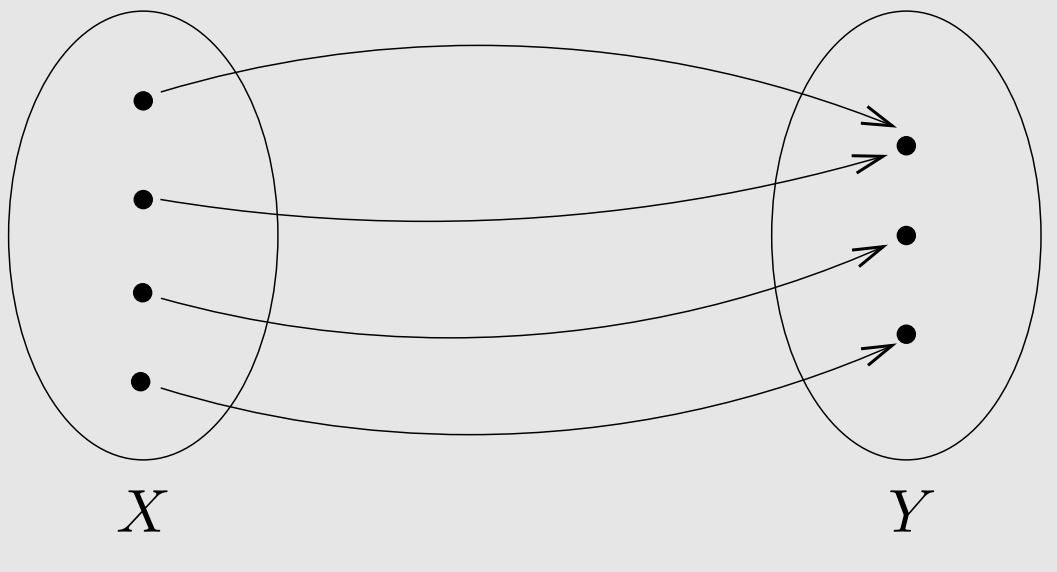
\includegraphics[width=0.75\linewidth]{Bilder/Surjektiv.JPG}
            \end{center}
        \end{minipage}
    \end{center}


    \begin{center}
        \begin{minipage}{0.5\linewidth}
            \subsubsection{Injektiv}

            $f$ heisst injektiv falls jedes $y \in Y$ \emph{höchstens} ein Urbild hat, d.h.:

            \begin{center}
                $\forall x_1, x_2 \in X : f(x_1) = f(x_2) \Rightarrow x_1 = x_2$
            \end{center}
        \end{minipage}
        \begin{minipage}{0.49\linewidth}
            \begin{center}
                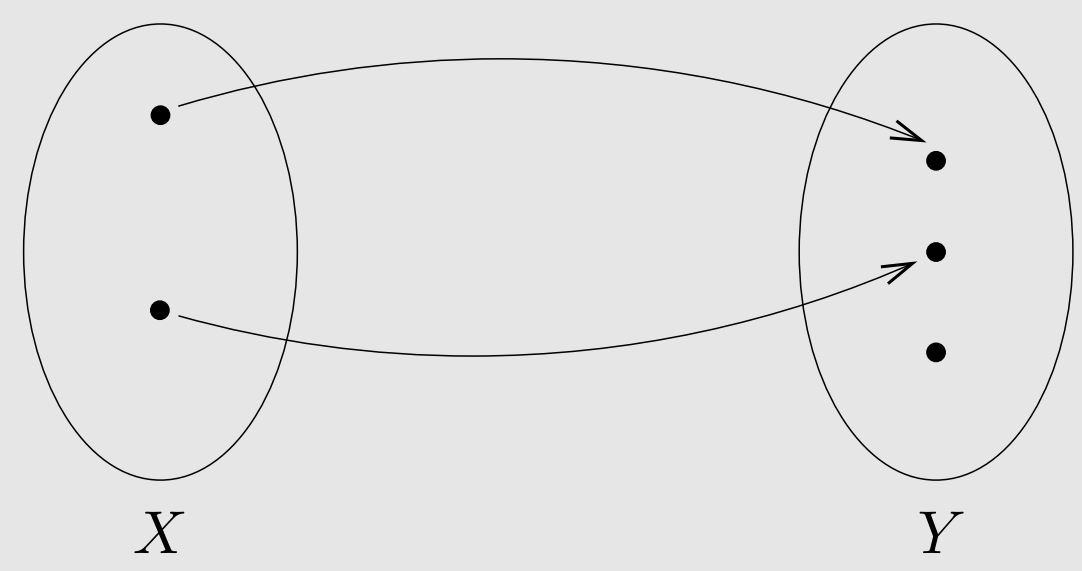
\includegraphics[width=0.75\linewidth]{Bilder/Injektiv.JPG}
            \end{center}
        \end{minipage}
    \end{center}

    \subsubsection{Bijektiv und Umkehrabbildung}

    $f$ heisst bijektiv, falls jedes $y \in Y$ \emph{genau} ein Urbild hat, d.h. $f$ ist surjektiv und injektiv.

    Ist $f$ bijektiv, dann kann man eine \emph{Umkehrabbildung} $f^{-1}$ einführen:

    \begin{center}
        \eqbox{$f^{-1}: Y \to X, \quad y \mapsto f(y)$}
    \end{center}


    \subsection{Reelle Zahlen}

    \begin{center}
        \begin{tabular}{r l} \toprule
            Natürliche Zahlen             & $\mathbb{N} = \{1, 2, 3, \dots\}, \, \mathbb{N}_0 = \{0, 1, 2, 3, \dots\}$ \\
            Ganze Zahlen                  & $\mathbb{Z} = \{\dots, -1, 0, 1, \dots\}$                                  \\
            Rationale Zahlen              & $\mathbb{Q} = \{\frac{p}{q}; p \in \mathbb{Z} \land q \in \mathbb{N}\}$    \\
            Irrationale Zahlen            & $\R \setminus \mathbb{Q}$                                                  \\
            Reelle Zahlen                 & $\R = \mathbb{Q} + \R \setminus \mathbb{Q}$                                \\ \midrule
            $[a,b]$                       & \hspace*{-10pt} $ := \{x \in \R; a \leq x \leq b\}$                        \\
            $]a,b[ \Leftrightarrow (a,b)$ & \hspace*{-10pt} $:= \{x \in \R; a < x < b\}$                               \\
            \bottomrule
        \end{tabular}
    \end{center}

    \subsubsection{Vollständigkeitsaxiom}

    $\R$ ist \emph{Ordnungsvollständig}, dass heisst: \eqbox{$\forall a, b \in \R \,\, \exists c \in \R: \, a \leq c \leq b$}

    \subsubsection{Dreiecksungleichung}

    Es gilt für alle $x,y \in \R$: \eqboxf{$| x + y | \leq | x | + | y |$}

    \subsubsection{Archimedisches Prinzip}

    Zu jeder Zahl $0 < b \in \R$ gibt es ein $n \in \mathbb{N}$ mit $b < n$. \medskip

    Daraus folgt: $\infty$ und $-\infty$ ist keine reelle Zahl.




    \subsubsection{Supremum und Infimum}


    \begin{center}
        \begin{minipage}{0.48\linewidth}
            Eine Menge $A \subset \R$ heisst nach oben beschränkt, falls gilt

            \begin{center}
                $\exists b \in \R \, \, \forall a \in A: a \leq b$
            \end{center}

            wobei $b$ eine obere Schranke genannt wird, die kleinste obere Schranke ist das \textbf{Supremum}.

            \begin{center}
                $\sup\limits_{x \in \R} A \Leftrightarrow \sup\{A; x \in \R\}$
            \end{center}

            Wird das Supremum angenommen in $A$, dann ist es das \textbf{Maximum}.

        \end{minipage}
        \,\vline\,
        \begin{minipage}{0.48\linewidth}
            Eine Menge $A \subset \R$ heisst nach unten beschränkt, falls gilt

            \begin{center}
                $\exists b \in \R \, \, \forall a \in A: a \geq b$
            \end{center}

            wobei $b$ eine untere Schranke genannt wird, die kleinste untere Schranke ist das \textbf{Infimum}.

            \begin{center}
                $\inf\limits_{x \in \R} A \Leftrightarrow \inf\{A; x \in \R\}$
            \end{center}

            Wird das Infimum angenommen in $A$, dann ist es das \textbf{Minimum}.

        \end{minipage}
    \end{center}


    \subsection{Potenzen und Wurzel}

    Sei $n,m \in \N$. Die reelle Wurzel ist definiert auf $\R^+$.

    \begin{center}
        \begin{minipage}{0.48\linewidth}
            \begin{center}
                \renewcommand{\arraystretch}{1.35}
                \begin{tabular}{r l}
                    $a^n \cdot a^m$    & \hspace*{-10pt}$= a^{n + m}$
                    \\
                    $\dfrac{a^n}{a^m}$ & \hspace*{-10pt}$= a^{n - m}$                   \\
                    $a^n \cdot b^n$    & \hspace*{-10pt}$= (a \cdot b)^n$               \\
                    $\dfrac{a^n}{b^n}$ & \hspace*{-10pt}$= \left(\dfrac{a}{b}\right)^n$ \\
                    $(a^n)^m$          & \hspace*{-10pt}$= a^{n \cdot m}$               \\
                    $b^0$              & \hspace*{-10pt}$= 1$                           \\
                \end{tabular}
            \end{center}
        \end{minipage}
        \,\vline\,
        \begin{minipage}{0.48\linewidth}
            \begin{center}
                \renewcommand{\arraystretch}{1.35}
                \begin{tabular}{r l}
                    $b^{\frac{n}{m}}$                  & \hspace*{-10pt}$= \sqrt[m]{b^n}$          \\
                    $b^{-1}$                           & \hspace*{-10pt}$= \dfrac{1}{b^n}$         \\
                    $\sqrt[n]{a} \cdot \sqrt[n]{b}$    & \hspace*{-10pt}$= \sqrt[n]{a \cdot b}$
                    \\
                    $\dfrac{\sqrt[n]{a}}{\sqrt[n]{b}}$ & \hspace*{-10pt}$= \sqrt[n]{\dfrac{a}{b}}$ \\
                    $\sqrt[n]{\sqrt[m]{a}}$            & \hspace*{-10pt}$= \sqrt[n \cdot m]{a}$    \\
                    $\sqrt[n]{1}$                      & \hspace*{-10pt}$= 1$                      \\
                \end{tabular}
            \end{center}
        \end{minipage}
    \end{center}

    \textbf{Achtung}: Beim Wurzel ziehen, immer $\pm$ vor der Wurzel!


    \subsection{Logarithmus}

    Der Logarithmus ist definiert auf $\R^+ \setminus {0}$. Eigenschaften:

    \begin{center}
        \begin{minipage}{0.47 \linewidth}
            \begin{center}
                \renewcommand{\arraystretch}{1.35}
                \begin{tabular}{r l}
                    $\log(a \cdot b)$               & \hspace*{-10pt}$= \log(a) + \log(b)$
                    \\
                    $\log\left(\dfrac{a}{b}\right)$ & \hspace*{-10pt}$= \log(a) - \log(b)$ \\
                    $\log(a^n)$                     & \hspace*{-10pt}$= n \cdot \log(a)$   \\
                \end{tabular}
            \end{center}
        \end{minipage}
        \,\vline\,
        \begin{minipage}{0.47 \linewidth}
            \begin{center}
                \renewcommand{\arraystretch}{1.35}
                \begin{tabular}{r l}
                    $e^{\log(a)}$ & \hspace*{-10pt}$= a$ \\
                    $\log(e)$     & \hspace*{-10pt}$= 1$ \\
                    $\log(1)$     & \hspace*{-10pt}$= 0$ \\
                \end{tabular}
            \end{center}
        \end{minipage}
    \end{center}

    Bemerkung: $x = e^n \Leftrightarrow \log(x) = n$


    \subsection{Die Exponentialfunktion ($\exp(x) = e^x$)}

    \begin{center}
        \renewcommand{\arraystretch}{1.35}
        \begin{minipage}{0.47 \linewidth}
            \begin{center}
                \begin{tabular}{r l}
                    $e^{z + w}$    & \hspace*{-10pt}$= e^z \cdot e^w$  \\
                    $e^{-x}$       & \hspace*{-10pt}$= \dfrac{1}{e^x}$ \\
                    $\exp^{-1}(y)$ & \hspace*{-10pt}$= \log(y)$        \\
                \end{tabular}
            \end{center}
        \end{minipage}
        \,\vline\,
        \begin{minipage}{0.47 \linewidth}
            \begin{center}
                \renewcommand{\arraystretch}{1.35}
                \begin{tabular}{r l}
                    $\lim\limits_{x \to \infty} e^x$  & \hspace*{-10pt}$= \infty$ \\
                    $e^0$                             & \hspace*{-10pt}$= 1$      \\
                    $\lim\limits_{x \to -\infty} e^x$ & \hspace*{-10pt}$= 0$      \\
                \end{tabular}
            \end{center}
        \end{minipage}
    \end{center}

    \subsubsection{Trigonometrische- und Hyperbelfunktionen}

    \begin{center}
        \renewcommand{\arraystretch}{2.5}
        \begin{minipage}{0.47 \linewidth}
            \begin{center}
                \begin{tabular}{r l}
                    $\sin(z)$ & \hspace*{-10pt}$= \dfrac{e^{iz} - e^{-iz}}{2i}$ \\
                    $\cos(z)$ & \hspace*{-10pt}$= \dfrac{e^{iz} + e^{-iz}}{2}$  \\
                \end{tabular}
            \end{center}
        \end{minipage}
        \begin{minipage}{0.47 \linewidth}
            \begin{center}
                \begin{tabular}{r l}
                    $\sinh(z)$ & \hspace*{-10pt}$= \dfrac{e^{z} - e^{-z}}{2}$ \\
                    $\cosh(z)$ & \hspace*{-10pt}$= \dfrac{e^{z} + e^{-z}}{2}$ \\
                \end{tabular}
            \end{center}
        \end{minipage}
    \end{center}




    \subsection{Vektoren}

    \begin{center}
        \renewcommand{\arraystretch}{1.25}
        \begin{tabular}{r l} \toprule
            Euklidischer Raum    & $\R^n = \{\vect{x} = (x_1, \dots, x_n); x_i \in \R\}$                                   \\
            Addition             & $\vect{x} + \vect{y} = (x_1 + y_1, \dots, x_n + y_n), \, x_i, y_i \in \R^n$             \\
            Skalarmultiplikation & $\lambda \vect{x} = (\lambda x_1, \dots, \lambda x_n), \, x _i\in \R^n, \lambda \in \R$ \\
            Skalarprodukt        & $\langle \vect{x}, \vect{y} \rangle = x_1 y_1 + \dots + x_n y_n$                        \\
            Euklidische Norm     & $|| x || := \sqrt{\displaystyle\sum^n_{i = 1} x_i^2}$                                   \\ \bottomrule
        \end{tabular}
    \end{center}

    \subsubsection{Cauchy-Schwarz}

    Für alle $\vect{x}, \vect{y} \in \R^n$ gilt:

    \begin{center}
        \eqbox{$| \vect{x} \cdot \vect{y} | \leq || \vect{x} || \cdot || \vect{y} ||$}
    \end{center}


    \subsection{Komplexe Zahlen}

    \begin{center}
        \eqbox{$\mathbb{C} := \{a + i b: a,b \in \R\}$} wobei \eqboxf{$i = \sqrt{-1}$}
    \end{center}

    \begin{center}
        \renewcommand{\arraystretch}{1.25}
        \begin{tabular}{r l} \toprule
            Realteil             & $\Re{z} = a = \dfrac{z + \overline{z}}{2}$                                                                                    \\
            Imaginärteil         & $\Im{z} = b = \dfrac{z - \overline{z}}{2i}$                                                                                   \\ \midrule
            Komplexe Konjugation & $\overline{z} = a - ib$                                                                                                       \\
                                 & $\overline{z_1 + z_2} = \overline{z_1} + \overline{z_2}$, \, $\overline{z_1 \cdot z_2} = \overline{z_1} \cdot \overline{z_2}$ \\ \midrule
            Addition             & $z_1 + z_2 = (a_1 + a_2) + i(b_1 + b_2)$                                                                                      \\
            Multiplikation       & $z_1 \cdot z_2 = (a_1 a_2 - b_1 b_2) + i(a_2 b_1 + a_1 b_2)$                                                                  \\
            Division             & $\dfrac{z_1}{z_2} = \dfrac{z_1 \cdot \overline{z_2}}{z_2 \cdot \overline{z_2}}$                                               \\ \midrule
            Absolutbetrag        & $| z | = \sqrt{z \overline{z}} = \sqrt{\Re{z}^2 + \Im{z}^2}$                                                                  \\
                                 & $|z_1 \cdot z_2| = |z_1| \cdot |z_2|$                                                                                         \\
            Phase                & $\varphi = \arctan \left( \dfrac{\Im{z}}{\Re{z}} \right)$                                                                     \\ \bottomrule
        \end{tabular}
    \end{center}

    \subsubsection{Eulersche Formel und Eulers Identität}

    \begin{center}
        \begin{minipage}{0.47 \linewidth}
            \begin{center}
                \eqboxf{$e^{i\varphi} = \cos\varphi + i \sin\varphi$}
            \end{center}
        \end{minipage}
        \begin{minipage}{0.47 \linewidth}
            \begin{center}
                \eqbox{$e^{i \pi} = -1$} \qquad \eqbox{$e^{2 \pi i} = 1$}
            \end{center}
        \end{minipage}
    \end{center}

    \subsubsection{Polarform}

    In der Polardarstellung $z = | z | e^{i\varphi}$ gelten folgende Rechenregel:

    \begin{center}
        \renewcommand{\arraystretch}{1.5}
        \begin{tabular}{r l} \toprule
            Realteil            & $\Re{z} = \cos(\varphi)$                                                                                               \\
            Imaginärteil        & $\Im{z} = \sin(\varphi)$                                                                                               \\
            \midrule
            Komplex Konjugation & \hspace*{-10pt} $\overline{z} = | z | e^{-i\varphi} = |z| \cdot (\cos\varphi - i\sin\varphi)$                          \\ \midrule
            Multiplikation      & \hspace*{-10pt} $z_1 \cdot z_2 = |z_1| \cdot |z_2| e^{i(\varphi_1+\varphi_2)}$                                         \\
            Division            & \hspace*{-10pt} $\dfrac{z_1}{z_2} = \dfrac{|z_1|}{|z_2|} \cdot e^{i(\varphi_1 - \varphi_2)}$                           \\
            \midrule
            Potenzieren         & \hspace*{-10pt} $(|z|e^{i\varphi})^n = |z|^n \cdot e^{i (n \cdot \varphi)}$                                            \\
            n-te Wurzel         & \hspace*{-10pt} $\sqrt[n]{z} = \sqrt[n]{|z|} \cdot e^{i(\frac{\varphi}{n} + \frac{2 \pi k}{n})}, \, k = 0, \dots, n-1$ \\
            \bottomrule
        \end{tabular}
    \end{center}




    \subsection{Fundamentalsatz der Algebra}

    Jedes Polynom $p(z)$ vom Grad $n \geq 1$ hat in $\mathbb{C}$ genau $n$ Nullstellen.

    \begin{center}
        $p(z) = z^n + a_{n-1}z^{n-1} + \dots + a_1 z + a_0$
    \end{center}

    Damit ist $\mathbb{C}$ im Unterschied zu $\R$ \textbf{algebraisch vollständig}.



    \subsection{Sonstiges}

    Bei Ungleichungen muss man bei einer \textbf{Multiplikation mit negativen Zahlen das Relationszeichen umdrehen}! \medskip

    Zum herausfinden einer Rekursivformel ist eine Primfaktorzerlegung sehr hilfreich!

    \subsubsection{Die Bernouillische Ungleichung}

    $\forall x \in \R, x \geq -1$ und $\forall n \in \N$ gilt:

    \begin{center}
        $(1 + x)^n \geq 1 + nx$
    \end{center}


    \subsubsection{Wallisches Produkt}

    Die irrationale Zahl $\pi$ wird approximiert durch:

    \begin{center}
        $\displaystyle \pi = \lim\limits_{n \to \infty} \dfrac{1}{n} \dfrac{(2^n n!)^4}{(2n!)^2}$
    \end{center}

    \subsubsection{Gerade und Ungerade Funktionen}

    Eine Funktion $f(t)$ heisst:

    \begin{center}
        \renewcommand{\arraystretch}{1.5}
        \begin{tabular}{l} \toprule
            i) \emph{gerade} falls $f(t) = f(-t)$ (Symmetrisch zur $y$-Achse).   \\
            ii) \emph{ungerade} falls $f(t) = -f(-t)$ (Punktsymm. zum Ursprung). \\
            \bottomrule
        \end{tabular}
    \end{center}

    Es gelten die folgenden Eigenschaften: \medskip

    - Das Produkt zweier geraden oder ungeraden Funktionen ist gerade.

    - Das Produkt einer geraden und ungeraden Funktion ist ungerade.

    - Falls $f(t)$ gerade ist, gilt $\int\limits_{-a}^{0} f(t) dt = \int\limits_{0}^{a} f(t) dt$.

    - Falls $f(t)$ ungerade ist, gilt $\int\limits_{-a}^{a} f(t) dt = 0$.




    \subsection{Trigonometrische Funktionen: Wertetabelle}

    \begin{center}
        \renewcommand{\arraystretch}{1.25}
        \begin{tabular}{r c c c c c} \toprule
            deg/rad & 0$^\circ$/0 & 30$^\circ$/$\frac{\pi}{6}$ & $45^\circ$/$\frac{\pi}{4}$ & 60$^\circ$/$\frac{\pi}{3}$ & 90$^\circ$/$\frac{\pi}{2}$ \\ \midrule
            sin     & $0$         & $\frac{\sqrt{1}}{2}$       & $\frac{\sqrt{2}}{2}$       & $\frac{\sqrt{3}}{2}$       & $1$                        \\
            cos     & $1$         & $\frac{\sqrt{3}}{2}$       & $\frac{\sqrt{2}}{2}$       & $\frac{\sqrt{1}}{2}$       & $0$                        \\
            tan     & $0$         & $\frac{\sqrt{3}}{3}$       & $1$                        & $\sqrt{3}$                 & -                          \\ \bottomrule
        \end{tabular}
        \begin{tabular}{r c c c c} \toprule
            deg/rad & 120$^\circ$/$\frac{2\pi}{3}$ & 135$^\circ$/$\frac{3\pi}{4}$ & $150^\circ$/$\frac{5\pi}{6}$ & 180$^\circ$/$\pi$ \\ \midrule
            sin     & $\frac{\sqrt{3}}{2}$         & $\frac{\sqrt{2}}{2}$         & $\frac{1}{2}$                & $0$               \\
            cos     & $- \frac{1}{2}$              & $- \frac{\sqrt{2}}{2}$       & $- \frac{\sqrt{3}}{2}$       & $-1$              \\
            tan     & $-\sqrt{3}$                  & $- 1$                        & $-\frac{\sqrt{3}}{3}$        & $0$               \\ \bottomrule
        \end{tabular}
    \end{center}


    \subsection{Trigonometrische und Hyperbolische Identitäten}

    \begin{center}
        \begin{minipage}{0.47 \linewidth}
            \begin{center}
                \eqboxf{$cos^2(x) + sin^2(x) = 1$} \medskip

                \eqbox{$\tan(x) = \dfrac{\sin(x)}{\cos(x)}$}
            \end{center}
        \end{minipage}
        \begin{minipage}{0.47 \linewidth}
            \begin{center}
                \eqbox{$\cosh^2(x) - \sinh^2(x) = 1$} \medskip

                \eqbox{$\tanh(x) = \dfrac{\sinh(x)}{\cosh(x)}$}
            \end{center}
        \end{minipage}
    \end{center}

    \subsubsection{Trigonometrische Additionstheoreme}

    \begin{center}
        \renewcommand{\arraystretch}{1.5}
        \begin{tabular}{l l} \toprule
            \multicolumn{2}{l}{$\cos(x\pm y)=\cos(x)\cos(y)\mp\sin(x)\sin(y)$}                                                  \\
            \multicolumn{2}{l}{$\sin(x\pm y)=\sin(x)\cos(y)\pm\cos(x)\sin(y)$}                                                  \\
            \midrule
            $\cos \left(x+\frac{1}{2} \pi\right)=-\sin (x)$  & \hspace*{-10pt} $\sin \left(x+\frac{1}{2} \pi\right)=\cos (x)$   \\
            \midrule
            \multicolumn{2}{l}{$\sin(x)\sin(y)=\frac{1}{2}(\cos(x-y)-\cos(x+y))$}                                               \\
            \multicolumn{2}{l}{$\cos(x)\cos(y)=\frac{1}{2}(\cos(x-y)+\cos(x+y))$}                                               \\
            \multicolumn{2}{l}{$\sin(x)\cos(y)=\frac{1}{2}(\sin(x-y)+\sin(x+y))$}                                               \\
                \midrule
            $\sin^2(x)=\frac{1}{2}(1-\cos(2x))$              & \hspace*{-10pt} $\cos^2(x)=\frac{1}{2}(1+\cos(2x))$              \\
            $\sin^{3}(x)=\frac{1}{4}(3 \sin (x)-\sin (3 x))$ & \hspace*{-10pt} $\cos^{3}(x)=\frac{1}{4}(3 \cos (x)+\cos (3 x))$ \\
            \bottomrule
        \end{tabular}
    \end{center}

    \subsubsection{Hyperbolische Additionstheoreme}

    \begin{center}
        \renewcommand{\arraystretch}{1.5}
        \begin{tabular}{l l} \toprule
            \multicolumn{2}{l}{$\sinh(x \pm y) = \sinh(x) \cosh(y) \pm \cosh(x) \sinh(y)$} \\
            \multicolumn{2}{l}{$\cosh(x \pm y) = \cosh(x) \cosh(y) \pm \sinh(x) \sinh(y)$} \\
            \midrule
            $\cosh(x) = \cos(ix)$              & $\sinh(x) = -i \sin(ix)$                  \\
            \midrule
            $\sinh^2(x)=\frac{\cosh(2x)-1}{2}$ & $\cosh^2(x)=\frac{\cosh(2x)+1}{2}$        \\
            \bottomrule
        \end{tabular}
    \end{center}


    \subsection{Berechnen von Grenzwerten}
    \subsubsection{Dominanzen}
    Die Sachen die links stehen wachsen langsamer als die Sachen die rechts stehen:\\
    $\log{(n)}\prec\log^2{(n)}\prec\dots\prec\ n^{\frac{1}{3}}\prec\sqrt{n}\prec n\prec n^2\prec\dots\prec e^n\prec n!\prec n^n$
    \subsubsection{Brüche}
    \begin{center}
        $x \rightarrow \infty : \hspace*{10pt}$ Durch die groesste Potenz des Zaehlers/Nenners teilen
        $x \rightarrow 0 : \hspace*{10pt}$ Durch die kleinste Potenz des Zaehlers/Nenners teilen
    \end{center}
    \subsubsection{Beträge}
    Beträge vereinfachen indem man sich überlegt, ob das Argument im Betrag grösser bzw. kleiner 0 ist\\\\
    \begin{example}
        \textbf{Beispiel}
        \begin{equation*}
            \lim_{x \rightarrow 2^-} \frac{4-x^2}{\vert x-2 \vert} = \lim_{x \rightarrow 2^-} \frac{4-x^2}{2-x} = \lim_{x \rightarrow 2^-} (2+x) = 4
        \end{equation*}
    \end{example}
    \subsubsection{Wurzelterme}
    Wurzelterme kann man meistens mithilfe der 3. binomischen Formel erweitern\\\\
    \begin{example}
        \textbf{Beispiel}
        \begin{equation*}
            \lim_{x \rightarrow \infty} \sqrt{x^2+x}-x = \lim_{x \rightarrow \infty} \frac{x^2+x-x^2}{\sqrt{x^2+x}+x} = \lim_{x \rightarrow \infty} \frac{1}{\sqrt{1+\frac{1}{x}}+1}=\frac{1}{2}
        \end{equation*}
    \end{example}
    \subsubsection{Beschränktheit einer Funktion}
    Man kann die Beschränktheit einer Funktion (v.a. trig. Fkt.) ausnutzen um Grenzwerte zu berechnen\\\\
    \begin{example}
        \textbf{Beispiel}
        \begin{equation*}
            \lim_{x \rightarrow 0} x^2 \sin \left(\frac{1}{x} \right) = 0
        \end{equation*}
    \end{example}
    \subsubsection{Sandwich-Theorem}
    Seien $(x_n),(y_n),(z_n)$ Folgen so dass $x_n\le y_n\le z_n$\\ mit $\lim_{n \rightarrow \infty} x_n= \lim_{n \rightarrow \infty} z_n=c$, dann muss auch $\lim_{n \rightarrow \infty} y_n=c $
    \subsubsection{Potenzreihen}
    Falls die Potenzreihe der Funktion bekannt ist, kann man sie durch die Potenzreihe darstellen
    \subsection{Bernouilli de l'Hôpital}

    Seien $f,g: [a,b] \to \R$ stetig und differenzierbar in $]a,b[$. Sei $g'(x_0) \neq 0$ für alle $x \in ]a,b[$ und $f(a) = 0 = g(a)$ oder $f(a) = \pm \infty = g(a)$. Existiert

    \begin{center}
        $\lim\limits_{x \to a^+} \dfrac{f'(x)}{g'(x)}$
    \end{center}

    Dann ist $g(x) \neq 0$ für alle $x > a$, und es gilt

    \begin{center}
        \eqboxf{$\lim\limits_{x \to a^+} \dfrac{f(x)}{g(x)} = \lim\limits_{x \to a^+} \dfrac{f'(x)}{g'(x)}$}
    \end{center}
    \subsubsection{''exp-log'' Methode}
    \begin{eq}
        \lim_{x \rightarrow x_0} g(x)^{h(x)}=\exp\left(\lim_{x \rightarrow x_0} h(x) \cdot \ln(g(x))\right)
    \end{eq}
    \begin{example}
        \textbf{Beispiel}
        \begin{align*}
            \lim_{x \rightarrow 0}(1+3\sin(x))^{\frac{1}{x}} & =\exp \left(\lim_{x \rightarrow 0} \frac{\ln(1+3\sin(x))}{x}\right)    \\
                                                             & =\exp \left(\lim_{x \rightarrow 0} \frac{3 \cos(x)}{1+3\sin(x)}\right) \\
                                                             & =e^3
        \end{align*}
    \end{example}
    \subsection{Wichtige Grenzwerte}

    \begin{center}
        \renewcommand{\arraystretch}{2}
        \begin{tabular}{l l l l l} \toprule
            $\lim\limits_{n \to \infty} (1 + \frac{1}{n})^n$                  & \hspace*{-10pt} $= e$      & \hspace*{+10pt}
            $\lim\limits_{n \to \infty} (1 + \frac{a}{n})^n$                  & \hspace*{-10pt}$= e^a$                       \\
            $\lim\limits_{n \to \infty} n ( a^{\frac{1}{n}} - 1)$             & \hspace*{-10pt}$= \log(a)$ & \hspace*{+10pt}
            $\lim\limits_{n \to 0} \frac{a^n - 1}{n}$                         & \hspace*{-10pt}$= \log(a)$                   \\
            $\lim\limits_{n \to \infty} \sqrt[n]{n}$                          & \hspace*{-10pt}$= 1$       & \hspace*{+10pt} \\
            \midrule
            $\lim\limits_{t \to \infty} t \sin(\frac{1}{t})$                  & \hspace*{-10pt}$= 1$       & \hspace*{+10pt}
            $\lim\limits_{t \to 0} \frac{\sin(t)}{t}$                         & \hspace*{-10pt}$= 1$                         \\
            $\lim\limits_{t \to \infty} t \log(1 + \frac{1}{t})$              & \hspace*{-10pt}$= 1$       & \hspace*{+10pt}
            $\lim\limits_{t \to 0} \frac{\log(1 + t)}{t}$                     & \hspace*{-10pt}$= 1$                         \\
            $\lim\limits_{t \to \infty} \frac{1}{t^2(1 - \cos(\frac{1}{t}))}$ & \hspace*{-10pt}$= 1$       & \hspace*{+10pt}
            $\lim\limits_{t \to 0} \frac{t^2}{1 - \cos(t)}$                   & \hspace*{-10pt}$= 2$                         \\
            $\lim\limits_{t \to \infty} \frac{1}{t \sin(\frac{1}{t})}$        & \hspace*{-10pt}$= 1$       & \hspace*{+10pt}
            $\lim\limits_{t \to 0} \frac{t}{\sin(t)}$                         & \hspace*{-10pt}$= 1$                         \\
            $\lim\limits_{t \to 0} \frac{e^t - 1}{t}$                         & \hspace*{-10pt}$= 1$       & \hspace*{+10pt}
            $\lim\limits_{t \to 0} \frac{\log(1 + 2t)}{\log(1 + t)}$          & \hspace*{-10pt}$= 2$                         \\
            \bottomrule
        \end{tabular}
    \end{center}


    \subsection{Tipps Grenzwertberechnung}

    Verschiedene mögliche Ansätze:

    \begin{itemize}
        \item Bei Grenzwerten, welche eingesetzt $\frac{0}{0}$ oder $\frac{\infty}{\infty}$ geben, L'hopital anwenden!
        \item Wurzelterme: 3te Binomische Formel versuchen
        \item Schwieriger $\lim\limits_{n \to 0} (\dots)$ : Taylorformel mit Entwicklungspunkt $0$ benutzen (getrennt für Nenner und Zähler anwenden!!!). Dies funktioniert, da die Approximation im Entwicklungspunkt exakt ist.
        \item Grenzwerten mit vielen Funktionen: So umformen zu versuchen, dass man die Grenzwerte unter 'Wichtige Grenzwerte' verwenden kann!
              \begin{itemize}
                  \item Bei $\lim\limits_{n \to \infty} (\dots)^n$ muss man fast immer ausschliesslich $e^{n \cdot log(\dots)}$ als erste Umformung benutzen!
              \end{itemize}
    \end{itemize}

    \subsubsection{Grenzwert und Kompositionen stetiger Funktionen}

    Wird der Grenzwert einer Komposition stetiger Funktionen genommen, so darf man den Grenzwert auf die innere Funktion anwenden. Beispiel:

    \begin{center}
        $\lim\limits_{x \to 0} \exp(\frac{1}{x}\log(\cos(x))) = \exp(\lim\limits_{x \to 0} \frac{1}{x}\log(\cos(x)) )$
    \end{center}

    \section{Folgen und Reihen}

    \subsection{Grenzwert einer Folge}

    Die Folge $(a_n)_{n \in \mathbb{N}}$ konvergiert gegen den Grenzwert $a$ für $n \to \infty$, falls
    \begin{center}
        \eqboxf{$\forall \epsilon > 0 \,\, \exists N(\epsilon) \in \mathbb{N} \text{ so dass } \forall n \geq N: | a_n - a | < \epsilon$}
    \end{center}

    Wenn dies gilt, schreibt man: $\liminfty{n} a_n = a$ oder $a_n \to a (n \to \infty)$

    \begin{center}
        \begin{minipage}{0.5\linewidth}
            \begin{center}
                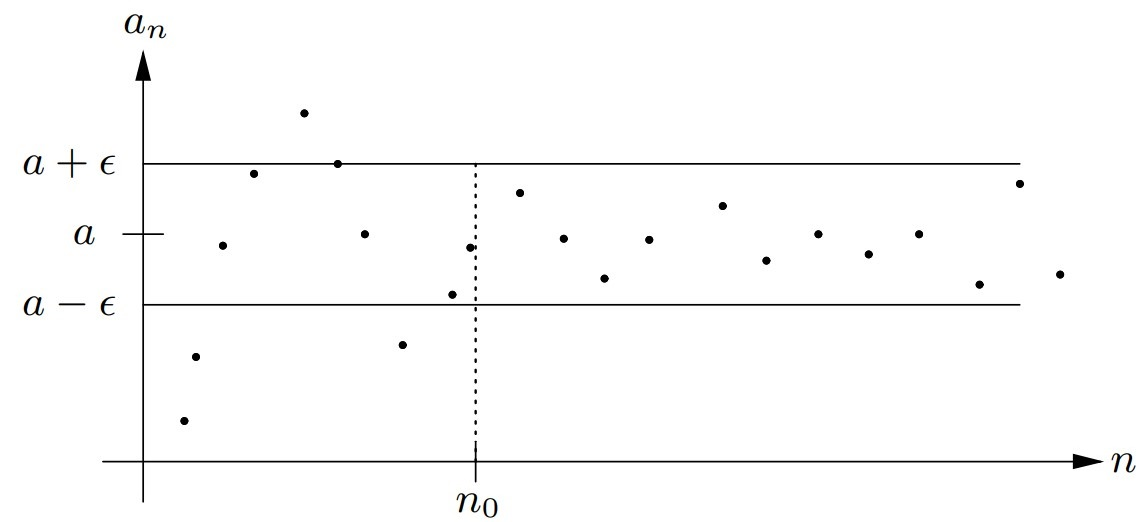
\includegraphics[width=1\linewidth]{Bilder/z_02.jpg}
            \end{center}
        \end{minipage}
        \begin{minipage}{0.47 \linewidth}
            i) Eine Folge heisst \emph{konvergent}, falls sie einen Grenzwert besitzt. \medskip

            ii) Besitzt die Folge keinen Grenzwert heisst sie \emph{divergent}.
        \end{minipage}
    \end{center}


    \subsection{Monotonie bei Folgen}

    Eine Folge $(a_n)_{n \in \N}$ bzw. $n \mapsto a_n$ heisst ..., wenn

    \begin{center}
        \renewcommand{\arraystretch}{1.25}
        \begin{tabular}{r l} \toprule
            monoton wachsend:        & $a_1 \leq a_2 \leq \dots \leq a_{n-1} \leq a_n$ \\
            monoton fallend:         & $a_1 \geq a_2 \geq \dots \geq a_{n-1} \geq a_n$ \\
            streng monoton wachsend: & $a_1 < a_2 < \dots < a_{n-1} < a_n$             \\
            streng monoton fallend:  & $a_1 > a_2 > \dots > a_{n-1} > a_n$             \\
            \bottomrule
        \end{tabular}
    \end{center}


    \subsection{Konvergenzkriterien}

    \subsubsection{Monotone Konvergenz}

    Sei $(a_n)_{n \in \N} \in A$ eine nach oben beschränkte monton wachsende Folge bzw. eine nach unten beschränkte monoton fallende Folge. Dann gilt

    \begin{center}
        \eqbox{$\liminfty{n} a_n = \begin{cases}
                    \sup\limits_{n \in \N}(A) & \text{falls monoton wachsend} \\
                    \inf\limits_{n \in \N}(A) & \text{falls monoton fallend}  \\
                \end{cases}$}
    \end{center}

    \subsubsection{Satz: Rechenregeln unter Konvergenzbedingung}

    Seien $(a_n)_{n \in \N}$, $(b_n)_{n \in \N}$ konvergent mit den Grenzwerten $a$ bzw. $b$. Dann

    \begin{center}
        \renewcommand{\arraystretch}{1.25}
        \begin{tabular}{r l} \toprule
            i)   & $\liminfty{n}(a_n + b_n) = \liminfty{n} a_n + \liminfty{n} b_n = a + b$                                      \\
            ii)  & $\liminfty{n}(a_n \cdot b_n) = \liminfty{n} a_n \cdot \liminfty{n} b_n = a \cdot b$                          \\
            iii) & Falls $\forall n: b \neq 0 \neq b_n$, dann gilt: $\liminfty{n} \left(\dfrac{a_n}{b_n}\right) = \dfrac{a}{b}$ \\
            iv)  & Falls $a_n \leq b_n$ für alle $n \in \mathbb{N}$, so ist auch $a \leq b$                                     \\ \bottomrule
        \end{tabular}
    \end{center}


    \subsection{Teilfolgen und Häufungspunkte}

    \subsubsection{Teilfolge}
    Eine Teilfolge ist eine Folge, die entsteht, wenn man von der ursprünglichen Folge nur bestimmte Glieder auswählt. \\
    Sei $l: N \to \N$ streng monoton wachsende Abzählung, dann ist $(a_{l(n)})_{n \in \N}$ eine \emph{Teilfolge} von $(a_n)_{n \in \N}$. \medskip

    \subsubsection{Häufungspunkt}

    Ein Punkt $a \in \R$ heisst \emph{Häufungspunkt} von $(a_n)_{n \in \N}$, falls $(a_n)_{n \in \N}$ gegen $a$ eine konvergente Teilfolge besitzt:

    \begin{center}
        $a = \lim\limits_{l \to \infty} a_{l(n)}$
    \end{center}

    $a$ ist ein Häufungspunkt von $(a_n)_{n \in \mathbb{N}}$, genau dann wenn
    \begin{center}
        \eqbox{$\forall \epsilon > 0 \, \, \forall n \in \mathbb{N} \,\, \exists \, l \geq n: | a - a_{l(n)} | < \epsilon$}
    \end{center}

    \subsubsection{Limes superior und inferior}

    Sei $(a_n)_{n \in \mathbb{N}}$ eine Folge, dann ist Limes superior und Limes inferior:

    \begin{center}
        \begin{minipage}{0.5\linewidth}
            \begin{center}
                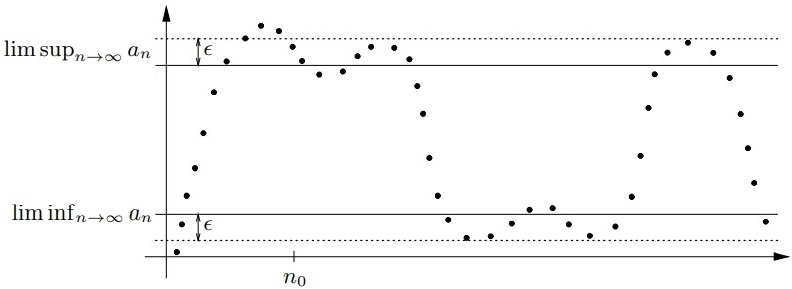
\includegraphics[width=1\linewidth]{Bilder/z_03.jpg}
            \end{center}
        \end{minipage}
        \begin{minipage}{0.47 \linewidth}
            \begin{center}
                \renewcommand{\arraystretch}{1.25}
                \begin{tabular}{r l} \toprule
                    $\liminf\limits_{n \to \infty} a_n$ & \hspace*{-10pt}$:= \sup\limits_{n \in \mathbb{N}}\inf\limits_{k \geq n} a_k$  \\
                    $\limsup\limits_{n \to \infty} a_n$ & \hspace*{-10pt}$:= \inf\limits_{n \in \mathbb{N}}\sup\limits_{k \geq n} a_k $ \\
                    \bottomrule
                \end{tabular}
            \end{center}
        \end{minipage}
    \end{center}

    wobei Limes superior und Limes inferior beides Häufungspunkte von $(a_n)_{n \in \N}$ sind. Ausserdem gilt: \medskip


    i) Eine beschränkte Folge konvergiert $\Leftrightarrow \limsup\limits_{n \to \infty} a_n = \liminf\limits_{n \to \infty} a_n$

    ii) Eine beschränkte Folge, welche nicht konvergiert, hat mindestens zwei
    Häufungspunkte.


    \subsubsection{Bolzano Weierstrass}

    \begin{center}
        \eqboxf{\begin{tabular}{C{0.89\linewidth}}
                Jede beschränkte Folge in $\R^d$ besitzt eine konvergente Teilfolge, also auch einen Häufungspunkt. \\
            \end{tabular}}
    \end{center}


    \subsection{Cauchy Folge und Cauchy-Kriterium}

    Eine Folge $(a_n)_{n \in \N}$ heisst \emph{Cauchy-Folge}, falls gilt

    \begin{center}
        \eqbox{$\forall \epsilon > 0 \,\, \exists n_0(\epsilon) \in \N \text{ s.d. } \forall m, n \geq n_0(\epsilon): |a_m - a_n| < \epsilon$}
    \end{center}

    D.h. wenn es zu jedem $\epsilon > 0$ einen Index $n_0(\epsilon)$ gibt, so dass ab diesem Index alle Folgenglieder weniger als $\epsilon$ voneinander entfernt sind.

    \subsection{Satz: Cauchy-Kriterium}

    Für $(a_n)_{n \in \N} \subset \R$ sind äquivalent:

    \begin{center}
        \eqboxf{$(a_n)_{n \in \N} \text{ konvergiert } \Leftrightarrow (a_n)_{n \in \N} \text{ ist Cauchy}$}
    \end{center}



    \subsection{Folgen in $\R^d$ oder $\mathbb{C}$}

    Sei $(\vect{a}_n)_{n \in \mathbb{N}}$ eine Folge in $\R^d$ mit $\vect{a}_n = (a^1_n, \dots, a^d_n) \in \R^d$. Es gilt

    \begin{center}
        \eqbox{$\liminfty{n} \vect{a}_n = \vect{a}$ falls $\liminfty{n} || \vect{a}_n - \vect{a} || = 0$}
    \end{center}

    Es sind äquivalent: $\liminfty{n} \vect{a}_n = \vect{a}  \Leftrightarrow \forall i \in \{1, \dots, d\}:  \liminfty{n} a_n^i = a^i$

    \subsubsection{Beschränkt in $\R^d$}

    Eine  vektorwertige Folge $(\vect{a}_n)_{n \in \mathbb{N}} \subset \R^d$ ist \emph{beschränkt}, falls gilt

    \begin{center}
        \eqbox{$\exists \, C \in \R \text{ so dass } \forall n \in \mathbb{N}: ||\vect{a}_n|| \leq C$}
    \end{center}


    \subsection{Reihen}

    Sei $(a_k)_{k \in \N}$ eine Folge. Die Folge $(S_n)_{n \in \mathbb{N}}$ der \emph{Partialsummen} ist

    \begin{center}
        $\displaystyle S_n = a_1 + \dots + a_n = \sum\limits^n_{k = 1} a_k, \quad n \in \N$
    \end{center}

    Man sagt die Reihe ist \emph{konvergent}, falls $\liminfty{n} S_n = \sum\limits^\infty_{k = 1} a_k$ existiert.

    \subsubsection{Cauchy Kriterium}

    Die Reihe $\sum\limits_{k=1}^\infty a_k$ ist konvergent \emph{genau dann, wenn} gilt:

    \begin{center}
        \eqbox{$\left| \sum\limits_{k = n+1}^m a_k \right| \to 0 \qquad (n \geq l, l \to \infty)$}
    \end{center}


    \subsection{Konvergenzkriterien für Reihen}

    Die Bedingung Nullfolge ($a_k \xrightarrow[]{k \to \infty} 0$) ist \textbf{notwendig}, aber \emph{nicht} hinreichend für die Konvergenz einer Reihe.

    \subsubsection{Quotientenkriterium}

    Sei $(a_k)_{k \in \N}$ eine Folge in $\R$ oder $\C$. Sei $a_k \neq 0$ und $k \in \N$. Es gilt:

    \begin{center}
        \eqbox{$\liminfty{k} \left| \dfrac{a_{k+1}}{a_k} \right| = \begin{cases}
                    < 1 & S_n \text{ konvergiert absolut}, \\
                    > 1 & S_n \text{ divergiert}           \\
                \end{cases}$}
    \end{center}

    \subsubsection{Wurzelkriterium}

    Sei $(a_k)_{k \in \N}$ eine Folge in $\R$ oder $\C$.

    \begin{center}
        \eqboxf{$\limsup\limits_{k \to \infty} \sqrt[k]{|a_k|} = \begin{cases}
                    < 1 & S_n \text{ konvergiert absolut}, \\
                    > 1 & S_n \text{ divergiert}           \\
                \end{cases}$}
    \end{center}

    \subsubsection{Minorantenkriterium}

    Sei $b_n \leq a_n$ und $\displaystyle \sum\limits_{n = 1}^\infty b_n$ divergent $\displaystyle \Rightarrow \sum\limits_{n = 1}^\infty a_n$ ist auch divergent.

    \subsubsection{Majorantenkriterium}

    Sei $|a_n| \leq b_n$ und $\displaystyle \sum\limits_{n = 1}^\infty b_n$ konvergent $\displaystyle \Rightarrow \sum\limits_{n = 1}^\infty a_n$ ist auch konvergent.


    \subsection{Absolute Konvergenz}

    Die Reihe $\displaystyle \sum\limits_{n = 1}^\infty a_n$ \emph{konvergiert absolut}, falls $\displaystyle \sum\limits_{n = 1}^\infty | a_n |$ konvergiert.


    \subsubsection{Satz}

    Seien die Reihen $\displaystyle \sum\limits_{n = 1}^\infty a_n$ und $\displaystyle \sum\limits_{k = 1}^\infty b_k$ absolut konvergent. Dann konvergiert die Reihe der Produkte absolut mit

    \begin{center}
        \eqbox{$\displaystyle \sum\limits_{n,k = 1}^\infty a_n b_k = \sum\limits_{n = 1}^\infty a_n \cdot \sum\limits_{k = 1}^\infty b_k$}
    \end{center}

    unabhängig von der Summationsreihenfolge.


    \subsection{Satz: Leibnitzkriterium}

    Sei $(a_n)_{n \in \N}$ eine monoton fallende, reelle \emph{Nullfolge}. Dass heisst

    \begin{center}
        \eqbox{$a_{n + 1} \leq a_n \quad \forall n \in \N_0$ und $\lim\limits_{n \to \infty} a_n = 0$}
    \end{center}

    Dann ist die Reihe $\displaystyle \sum\limits_{n = 0}^\infty (-1)^n a_n$ konvergent.


    \subsection{Standard Reihenabschätzung}

    \begin{center}
        \eqbox{$\displaystyle \left| \sum\limits_{k = 1}^n a_k \right| \leq n \cdot \max\limits_{1 \leq k \leq n} | a_k |$}
    \end{center}


    \subsection{Geometrische Reihe}

    Die Geometrische Reihe ist für $|z| < 1$ konvergent und es gilt:

    \begin{center}
        \eqboxf{$\displaystyle\sum\limits_{k = 0}^\infty z^k = \dfrac{1}{1-z}$} \qquad\qquad \eqbox{$\displaystyle\sum\limits_{k = 0}^n z^k = \dfrac{1 - z^{n + 1}}{1 - z}$}
    \end{center}


    \subsection{Wichtige Reihen}

    \begin{tabular}{r c l} \toprule
        Harmonische Reihe:           & \hspace*{-10pt} $\displaystyle\sum\limits^\infty_{k = 1} \dfrac{1}{k}$             & divergent                                                                               \\
        Riemann'sche $\zeta$-Funkt.: & \hspace*{-10pt} $\displaystyle\zeta(s) =\sum\limits^\infty_{k = 1} \dfrac{1}{k^s}$ & $\begin{cases} 0 < s \leq 1 & \text{divergent} \\ 1 < s & \text{konvergent}\end{cases}$ \\
        \bottomrule
    \end{tabular}


    \subsection{Wichtige Potenzreihen}

    Folgende Funktionen besitzen für alle $z \in \C$ konvergente Potenzreihen:

    \begin{center}
        \renewcommand{\arraystretch}{1.5}
        \begin{minipage}{0.47 \linewidth}
            \begin{center}
                \begin{tabular}{r l}
                    $\exp(z)$ & \hspace*{-10pt}$ := \displaystyle\sum\limits_{n = 0}^\infty \dfrac{z^n}{n!}$                 \\
                    $\sin(z)$ & \hspace*{-10pt}$:= \displaystyle\sum\limits_{n = 0}^\infty (-1)^n \dfrac{z^{2n+1}}{(2n+1)!}$ \\
                    $\cos(z)$ & \hspace*{-10pt}$:= \displaystyle\sum\limits_{n = 0}^\infty (-1)^n \dfrac{z^{2n}}{(2n)!}$     \\
                \end{tabular}
            \end{center}
        \end{minipage}
        \begin{minipage}{0.47 \linewidth}
            \begin{center}
                \begin{tabular}{r l}
                    $\sinh(z)$ & \hspace*{-10pt}$:= \displaystyle\sum\limits_{n = 0}^\infty \dfrac{z^{2n+1}}{(2n+1)!}$ \\
                    $\cosh(z)$ & \hspace*{-10pt}$:= \displaystyle\sum\limits_{n = 0}^\infty \dfrac{z^{2n}}{(2n)!}$     \\
                \end{tabular}
            \end{center}
        \end{minipage}
    \end{center}



    \subsection{Potenzreihen}

    Sei $z \in \C$. Eine Reihe der folgenden Form nennt man eine Potenzreihe:

    \begin{center}
        \eqbox{$\displaystyle p(z) := c_0 + c_1 z + c_2 z^2 + \dots = \sum\limits_{k = 0}^\infty c_k z^k$}
    \end{center}

    \subsubsection{Konvergenzradius}

    Eine Potenzreihe ist konvergent für alle $|z| < \rho$ und es gilt:

    \begin{center}
        \eqboxf{$\rho := \dfrac{1}{\limsup\limits_{k \to \infty} \sqrt[k]{|c_k|}}$} $\begin{cases}
                |z| < \rho & \text{konvergiert absolut} \\
                |z| = \rho & \text{keine Aussage}       \\
                |z| > \rho & \text{divergiert}          \\
            \end{cases}$
    \end{center}

    Innerhalb von $\rho$ darf man Limes, Ableitung, Integral austauschen!


    \subsubsection{Potenzreihen konvergieren gleichmässig}

    Sei eine Potenzreihe $p(z)$ mit Konvergenzradius $\rho > 0$. Dann konvergiert

    \begin{center}
        \eqbox{$\displaystyle p_n(z) = \sum\limits_{k = 0}^{n - 1} a_k z^k$}
    \end{center}

    gleichmässig gegen $p(z)$ auf $B_r(0)$ für jedes $r < p$.


    \subsubsection{Potenzreihen sind stetig}

    Potenzreihen sind \emph{stetig} im Inneren ihres Konvergenzradius $\rho$.


    \subsubsection{Potenzreihen sind differenzierbar}

    Eine Potenzreihe $f(x) = \sum\limits_{k = 0}^{\infty} a_k x^k$ ist im Inneren ihres Konvergenzradius \emph{gliedweise} differenzierbar. Die Ableitung von $f(x)$ ist

    \begin{center}
        \eqbox{$\displaystyle f'(x) = \sum\limits_{k = 1}^{\infty} k a_k x^{k - 1}$}
    \end{center}

    Ausserdem bestizt die Ableitung $f'(x)$ den \emph{gleichen} Konvergenzradius. \medskip

    \textbf{Achtung}: Oft ist es sinnvoll die Ableitungen der einzelnen Potenzen kurz anzuschauen, damit man die Formel nicht falsch anwendet!


    \subsubsection{Potenzreihen sind integrierbar}

    Eine Potenzreihen $f(x) = \sum\limits_{k = 0}^{\infty} a_k x^k$ ist innerhalb ihres Konvergenzradius \emph{gliedweise} integrierbar. Das Integral von $f(x)$ ist

    \begin{center}
        \eqbox{$\displaystyle \int\limits f(x) dx = \sum\limits_{k = 0}^{\infty} \dfrac{a_k}{k + 1} x^{k + 1}$}
    \end{center}

    und die Stammfunktion $F(x)$ besitzt den \emph{gleichen} Konvergenzradius $\rho$. \medskip

    \textbf{Achtung}: Oft ist es sinnvoll das Integral mit den einzelnen Potenzen kurz anzuschauen, damit man die Formel nicht falsch anwendet!
    \subsection{Cauchy-Produktformel}
    Sind $\sum_{n=0}^{\infty}a_n$ und $	\sum_{n=0}^{\infty}b_n$	absolut konvergente Reihen, dann gilt
    \begin{equation*}
        \sum_{n=0}^{\infty}c_n=\left(\sum_{n=0}^{\infty}a_n\right)\cdot\left(\sum_{n=0}^{\infty}b_n\right)=\sum_{n=0}^{\infty}\sum_{k=0}^{n}a_kb_{n-k}
    \end{equation*}

    \section{Stetigkeit auf $\R$ und $\R^d$}


    \subsection{Grenzwert einer Funktion}

    \subsubsection{Der Abschluss}

    Sei $\Omega \in \R^d$. Der Abschluss von $\Omega$ ist die Menge:

    \begin{center}
        \eqbox{$\overline{\Omega} = \{x \in \R^d; \exists (x_k)_{k \in \N} \subset \Omega, \, \lim\limits_{k \to \infty} x_k = x \}$}
    \end{center}

    In Worten formuliert: Der Abschluss sind alle Punkte $x_0$, die durch Punkte in $\Omega$ erreichbar sind. \medskip

    Bem: Offenbar gilt $\Omega \subset \overline{\Omega}$.

    \subsubsection{Definition: Grenzwert einer Funktion}

    Sei $\Omega \subset \R^d$, $f: \Omega \to \R^n$ und $x_0 \in \overline{\Omega}$. $f$ hat an der Stelle $x_0$ den \emph{Grenzwert} $a \in \R^n$, falls für jede Folge $(x_k)_{k \in \N}$ in $\Omega$ mit

    \begin{center}
        $x_k \xrightarrow[]{k \to \infty} x_0$ gilt $f(x_k) \xrightarrow[]{k \to \infty} a$.
    \end{center}

    Ist dies der Fall und $x_0 \in \Omega$, dann muss gelten $\lim\limits_{x \to x_0} f(x) = f(x_0)$.

    \subsubsection{Stetig in $x_0$ und stetig ergänzbar}

    Sei $\Omega \subset \R^d$, $f: \Omega \to \R^n$. Man sagt: \medskip

    i) Sei $x_0 \in \Omega$. $f$ ist \emph{stetig} in $x_0$, falls $f$ in $x_0$ einen Grenzwert besitzt. \medskip

    ii) Sei $x_0 \in \overline{\Omega} \setminus \Omega$. $f$ heisst an der Stelle $x_0$ \emph{stetig ergänzbar}, falls $f$ in $x_0$ einen Grenzwert besitzt. Notation: $\lim\limits_{k \to \infty} f(x_k) = a \, \Leftrightarrow \, \lim\limits_{\substack{x \to x_0 \\ x \neq x_0}} = a$


    \subsection{Für $\R$: Links- und Rechtsseitiger Grenzwert}

    \begin{center}
        \begin{minipage}{0.48\linewidth}
            Nähert man sich von Links an $x_0$ an, d.h. $x < x_0$ dann gilt:

            \begin{center}
                \eqbox{$f(x_0^-) := \lim\limits_{x \to x_0^-} f(x)$}
            \end{center}
        \end{minipage}\,\,
        \begin{minipage}{0.48\linewidth}
            Nähert man sich von Rechts an $x_0$ an, d.h. $x > x_0$ dann gilt:

            \begin{center}
                \eqbox{$f(x_0^+) := \lim\limits_{x \to x_0^+} f(x)$}
            \end{center}
        \end{minipage}
    \end{center}

    $f$ ist stetig an der Stelle $x_0$ genau dann, wenn $f(x_0^-) = f(x_0^+) = f(x_0)$.

    \subsubsection{Satz}

    Sei $]a,b[ \to \R$ monoton wachsend oder monoton fallend. Dann existieren für jedes $x_0 \in ]a,b[$ die links- und rechtsseitigen Grenzwerte.


    \subsection{Für $\R$: Monotonie bei Funktionen}

    $f:[a,b] \to \R$ heisst streng monoton wachsend, falls gilt

    \begin{center}
        \eqbox{$a \leq x < y \leq b \Rightarrow f(x) < f(y)$}
    \end{center}

    $f:[a,b] \to \R$ heisst streng monoton fallend, falls gilt

    \begin{center}
        \eqbox{$a \leq x < y \leq b \Rightarrow f(x) > f(y)$}
    \end{center}


    \subsection{Für $\R^d$: Grenzwert in $\R^d$}

    Sei $(x_k)_{k \in \N} \in \R^d$. Die Folge $x_k$ konvergiert gegen $x$, falls

    \begin{center}
        \eqbox{$\lim\limits_{k \to \infty} ||x_k - x|| = 0 \, \Leftrightarrow \, \lim\limits_{k \to \infty} x_k^j = x^j$}
    \end{center}

    wobei $x_k = (x^1_k, \dots, x^d_k)$ und $x = (x^1, \dots, x^d)$ beide in $\R^d$ definiert sind.
    \\ \textbf{Trick}: In $R^d$ kann in Polarkoordinaten substituiert werden und der Grenzwert berechnet werden: Wenn der
    Grenzwert nur von $r$ abhängt, dann ist die Funktion stetig.
    \subsection{Stetige Funktionen}

    Sei $\Omega \subset \R^d$, $f: \Omega \to \R^n$. Dann sagt man:

    \begin{center}
        $f$ heisst \textbf{stetig auf} $\Omega \subset \R$, falls $f$ in jedem Punkt $x_0 \in \Omega$ stetig ist.
    \end{center}

    \subsubsection{Satz: Vektorraum $C^0(\Omega, \R)$}

    Sei $\alpha, \beta \in \R$ und $f,g: \Omega \subset \R^d \to \R^n$ stetig. Dann ist $\alpha f + \beta g$ auch stetig. Die stetigen Funktionen $f: \Omega \to \R^n$ bilden also einen $\R$-Vektorraum.

    \begin{center}
        Notation: \eqbox{$C^0(\Omega, \R) = \{ f: \Omega \to \R^n; f \text{ ist stetig} \}$}
    \end{center}

    \subsubsection{Satz}

    Sind $f,g \in C^0(\Omega \subset \R^d, \R^n)$. So ist auch $f \circ g \in C^0(\Omega \subset \R^d, \R^n)$.


    \subsection{Lipschitz stetig}

    Sei $f: \Omega \subset \R^d \to \R^n$. $f$ heisst \emph{L-Lipschitz stetig} mit der Lipschitzkonstante $0 \leq L$, falls

    \begin{center}
        \eqbox{$\forall \vect{x},\vect{y} \in \Omega$ gilt $||f(\vect{x}) - f(\vect{y}) || \leq L \cdot || \vect{x} - \vect{y} ||$}
    \end{center}

    Bemerkung: Lipschitz stetig $\Rightarrow$ Gleichmässig stetig $\Rightarrow$ $f$ ist stetig


    \subsubsection{Satz}

    $f: \Omega \subset \R^d \to \R^n$ \emph{L-Lipschitz stetig} $\Rightarrow$ $f$ ist stetig ergänzbar in $x_0 \in \overline{\Omega}$.


    \subsection{Kompakt}

    $K \subset \R^d$ heisst kompakt, falls jede Folge $(x_k)_{k \in \N} \subset K$ einen Häufungs-punkt in $K$ besitzt. Ausserdem gilt folgende Äquivalenz:

    \begin{center}
        \eqbox{K kompakt $\Leftrightarrow$ $K$ ist beschränkt und abgeschlossen.}
    \end{center}

    Bem: Das eine Menge nicht Kompakt ist, zeigt man am besten, indem man eine unbeschränkte Folge findet (Folge ohne HP).


    \subsubsection{Lemma}

    Sei $K \subset \R$ kompakt. Dann ist $K$ beschränkt und es $\exists a,b \in K$ mit

    \begin{center}
        \eqbox{$-\infty < a = \inf(K) = \min(K) \qquad\quad \max(K) = \sup(K) = b < \infty$}
    \end{center}


    \subsubsection{Satz: Extremumsatz}

    Sei $K \subset \R^d$ kompakt, $f: K \to \R^n$ stetig. Dann ist auch das Bild der Funktion $f: K \to \R^n$ kompakt. Insbesondere gilt:

    \begin{center}
        \eqboxf{$f: K \to \R^n$ nimmt ihr \emph{Maximum und Minimum} auf $K$ an}
    \end{center}


    \subsection{Für $\R$: Weierstrass'sches Kriterium für Stetigkeit}

    $f: \Omega \in \R$ ist an der Stelle $x_0$ stetig \emph{genau dann, wenn}

    \begin{center}
        \eqboxf{$\forall \epsilon > 0 \,\, \exists \delta > 0 \text{ s.d. } \forall x \in \Omega: \, |x - x_0| < \delta \Rightarrow ||f(x) - f(x_0) || < \epsilon$}
    \end{center}

    \begin{center}
        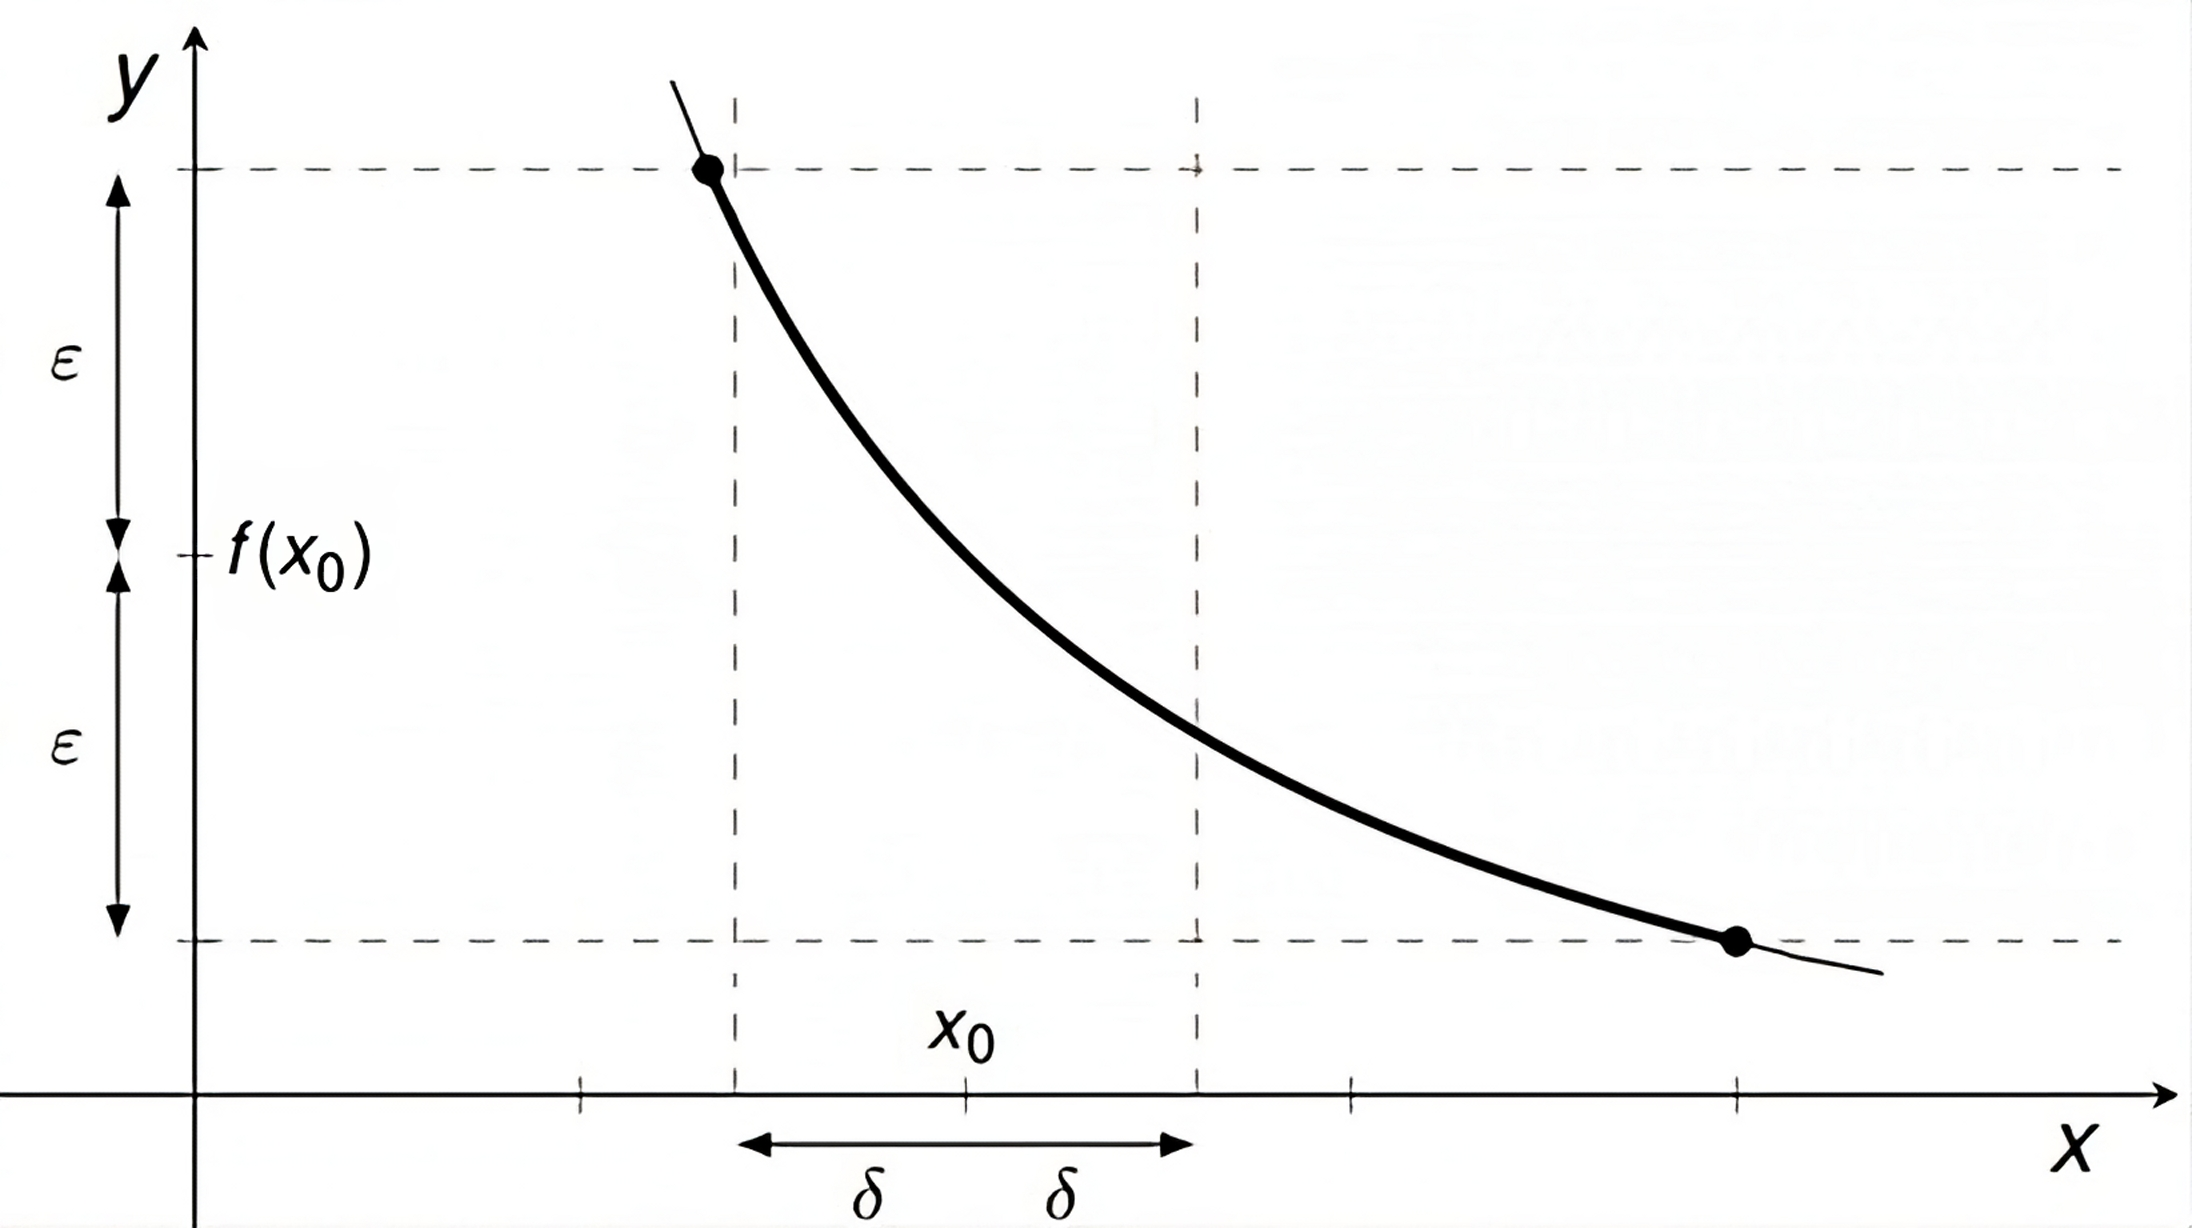
\includegraphics[width=0.75\linewidth]{Bilder/Delta_Epsilon_Kriterium.png}
    \end{center}
    \textbf{Vorgehen}: 	Wie finde ich zu jedem $\varepsilon > 0$ das passende  $\delta$?
    \begin{enumerate}
        \item Beginne mit $\left \vert f(x)-f(x_0) \right \vert < \varepsilon$ und finde einen Ausdruck so dass:
              $\left \vert f(x)-f(x_0) \right \vert \le ...\vert x-x_0 \vert ... < \varepsilon$
        \item Setze ein: $\vert x-x_0 \vert < \delta$
        \item $\left \vert f(x)-f(x_0) \right \vert \le ...\vert x-x_0 \vert ... <  ...\delta... <\varepsilon$
        \item Benutze $...\delta... <\varepsilon$ um $\delta(x_0, \varepsilon)$ zu finden
        \item Zeige, dass wirklich $\vert x-x_0 \vert < \delta \implies \left \vert f(x)-f(x_0) \right \vert < \varepsilon$
    \end{enumerate}


    \subsection{Für $\R$: Der Zwischenwertsatz}

    Sei $a < b$, $f:[a,b] \to \R$ stetig. Dann gilt

    \begin{center}
        \eqboxf{$\forall y \in [f(a),f(b)] \,\, \exists x \in [a,b]$ mit $f(x) = y$}
    \end{center}

    In Worten: ''Das Bild einer stetigen Funktion, die auf einem Intervall definiert ist, ist ein Intervall.''

    \subsubsection{Satz}

    Sei $f: [a,b] \to \R$ stetig und streng monoton wachsend/fallend. Setze $f(a) = c$ und $f(b) = d$. Dann gilt

    \begin{center}
        $f:[a,b] \to [c,d]$ ist bijektiv, und $f^{-1}$ ist stetig sowie streng monoton wachsend/fallend
    \end{center}


    \subsubsection{Satz}

    Sei $f:]a,b[ \to \R$ stetig und streng monoton wachsend/fallend mit

    \begin{center}
        $-\infty \leq c:= \lim\limits_{x \to a^+} f(x) < \lim\limits_{x \to b^-} f(x) =: d \leq \infty$
    \end{center}

    Dann ist $f:]a,b[ \to ]c,d[$ bijektiv, und $f^{-1}$ ist stetig sowie streng monoton wachsend/fallend.


    \subsection{Gleichmässige Stetigkeit}

    Sei $\Omega \subset \R^d$. $f: \Omega \to \R^n$ heisst gleichmässig stetig, falls gilt:

    \begin{center}
        \eqbox{$\forall \epsilon > 0 \,\, \exists \delta > 0 \text{ s.d. } \forall x,y \in \Omega: \, |x - y| \leq \delta \Rightarrow || f(x) - f(y) || < \epsilon$}
    \end{center}

    Bemerkung: Lipschitz stetig $\Rightarrow$ Gleichmässig stetig $\Rightarrow$ $f$ ist stetig

    \subsubsection{Satz}

    Sei $f: \Omega \subset \R^d \to \R^n$ gleichmässig stetig $\Rightarrow$ $f$ ist beschränkt auf $\Omega$.

    \subsubsection{Sätze}

    i) Sei $K \subset \R^d$ kompakt und $f \in C^0(K, \R^n) \Rightarrow f$ ist gleichmässig stetig. \medskip

    ii) Sei $f: \Omega \to \R^n$ gleichmässig stetig $\Rightarrow$ $f$ ist auf $\overline{\Omega}$ stetig ergänzbar. \medskip

    iii) Sei $\Omega \subset \R^d$ beschränkt, $f: \Omega \to \R^n$ stetig und auf $\overline{\Omega}$ stetig ergänzbar. $\Rightarrow$ $f$ ist gleichmässig stetig.




    \subsection{Punktweise und gleichmässige Konvergenz}


    \subsubsection{Supremumsnorm}

    Sei $f \in C^0(\Omega, \R^n)$. Dann ist die Supremumsnorm

    \begin{center}
        \eqbox{$||f||_{C^0} := \sup\limits_{x \in \Omega}|| f(x)|| < \infty$}
    \end{center}


    \subsubsection{Punktweise Konvergenz}

    Sei $\Omega \subset \R^d$, und $f, f_k: \Omega \to \R^n,\, k \in \N$. Die Folge $(f_k)_{k \in \N}$ konvergiert punktweise gegen $f$, falls

    \begin{center}
        \eqbox{$\forall x \in \Omega: \,\lim\limits_{k \to \infty} f_k(x) = f(x)$}
    \end{center}


    \subsubsection{Gleichmässige Konvergenz}

    Sei $\Omega \subset \R^d$, und $f, f_k: \Omega \to \R^n,\, k \in \N$. Die Folge $(f_k)_{k \in \N}$ konvergiert gleichmässig gegen $f$, falls

    \begin{center}
        \eqboxf{$\lim\limits_{k \to \infty} \sup\limits_{x \in \Omega} || f_k(x) - f(x) || = 0$}
    \end{center}

    Bemerkung: Gleichmässige Konvergenz $\Rightarrow$ Punktweise Konvergenz

    \subsubsection{Satz}

    Sei $f_k \in C^0(\Omega, \R^n)$ und $f_k$ konvergiert gleichmässig $\Rightarrow$ $f$ ist auf $\Omega$ stetig.


    \subsection{Einschub: De Morgansche Regeln}

    \begin{center}
        \renewcommand{\arraystretch}{1.5}
        \begin{minipage}{0.47 \linewidth}
            \begin{center}
                \eqbox{$(A_1 \cup A_2)^C = A_1^c \cap A_2^c$}
            \end{center}
        \end{minipage}
        \begin{minipage}{0.47 \linewidth}
            \begin{center}
                \eqbox{$(A_1 \cap A_2)^C = A_1^c \cup A_2^c$}
            \end{center}
        \end{minipage}
    \end{center}


    \section{Topologie}


    \subsection{Offene Mengen}

    \subsubsection{Der offene Ball}

    Sei $x_0 \in \R^d$ mit $r > 0$. Der offene Ball mit Radius $r$ und Zentrum $x_0$ ist

    \begin{center}
        \eqbox{$B_r(x_0) := \{x \in \R^d; ||x - x_0|| < r\}$}
    \end{center}

    \subsubsection{Definition: Offene Menge und Innerer Punkt}

    Ein Punkt $x_0 \in \Omega$ heisst \emph{innerer Punkt} von der Menge $\Omega$, falls

    \begin{center}
        \eqboxf{$\exists r > 0: B_r(x_0) \subset \Omega$}
    \end{center}

    Die Menge $\Omega \subset \R^d$ heisst \textbf{offen}, falls jedes $x_0 \in \Omega$ ein innerer Punkt ist.


    \subsubsection{Satz: Eigenschaften offener Mengen}

    Es gelten folgenden Eigenschaften für offene Mengen: \medskip

    i) $\Omega_1, \Omega_2 \subset \R^d$ offen $\Rightarrow$ Schnittmenge $\Omega_1 \cap \Omega_2$ ist offen. \medskip

    ii) $\Omega_l \subset \R^d$ offen, $l \in I$ $\Rightarrow$ $\bigcup\limits_{i \in I} \Omega_l$ offen.

    iii) Endliche offene Mengen $(A_i)_{i \in I} \Rightarrow \bigcap\limits_{i \in I} A_i$ offen.


    \subsection{Abgechlossene Mengen}

    Eine Menge $A \subset \R^d$ heisst \textbf{abgeschlossen}, falls das Komplement $A^C = \R^d \setminus A$ offen ist.

    \subsubsection{Satz: Eigenschaften abgeschlossener Mengen}

    i) $A_1, A_2$ abgeschlossen $\Rightarrow$ Vereinigungsmenge $A_1 \cup A_2$ abgeschlossen. \medskip

    ii) $A_l \subset \R^d$ abgeschlossen, $l \in I$ $\Rightarrow$ $\bigcap\limits_{i \in I} A_l$ abgeschlossen. \medskip

    iii) Endliche abgeschlossene Mengen $(A_i)_{i \in I} \Rightarrow \bigcup\limits_{i \in I} A_i$ abgeschlossen.


    \subsubsection{Bemerkungen}

    i) Die zwei Mengen $\R^n, \, \emptyset$ sind sowohl offen, als auch abgeschlossen. \medskip

    ii) Es gibt Mengen, die weder offen noch abgeschlossen sind!


    \subsection{Das Innere, der Abschluss und der Rand einer Menge}


    \subsubsection{Das Innere}

    Die Menge der inneren Punkte von $\Omega$

    \begin{center}
        \eqbox{$int(\Omega) = \overset{\circ}{\Omega} := \{x \in \Omega; \exists r > 0$ s.d. $B_R(x) \subset \Omega \} = \bigcup\limits_{U \subset \Omega, \text{ U offen}} U$}
    \end{center}

    heisst \textbf{offener Kern} oder das \textbf{Innere} von $\Omega$.


    \subsubsection{Der Abschluss}

    Der \textbf{Abschluss} einer Menge ist

    \begin{center}
        \eqbox{$clos(\Omega) = \overline{\Omega} := \bigcap\limits_{A \subset \Omega, \text{ A abgeschlossen}} A$} \medskip

        $\Leftrightarrow$ \eqbox{$\overline{\Omega} = \{x_0 \in \R^d; \, \exists (x_k)_{k \in \N} \subset \Omega, \, \lim\limits_{k \to \infty} x_k = x_0 \}$}
    \end{center}




    \subsubsection{Der Rand}

    Der \textbf{Rand} einer Menge ist

    \begin{center}
        \eqbox{$\partial\Omega := \overline{\Omega} \setminus \overset{\circ}{\Omega} = \{x \in \R^d; \forall r > 0: B_r(x) \,\cap\, \Omega \neq \emptyset \neq B_r(x) \setminus \Omega\}$}
    \end{center}


    \subsubsection{Satz: Eigenschaften}

    i) Der Rand $\partial \Omega$ ist abgeschlossen.

    ii) Aus $\overset{\circ}{\Omega} \subseteq \Omega \subseteq \overline{\Omega}$ folgt $\overline{\Omega} = \overset{\circ}{\Omega} \cup \partial \Omega$ und die Zerlegung ist disjunkt. \medskip

    iii) Es folgt das Kriterium: \eqboxf{$\Omega$ abgeschlossen $\Leftrightarrow \Omega = \overline{\Omega} \Leftrightarrow \partial \Omega \subset \Omega$}

    iv) Es gilt ausserdem $\overline{\overline{\Omega}} = \overline{\Omega}$, sowie $\overset{\circ}{\overset{\circ}{\Omega}} = \overset{\circ}{\Omega}$


    \subsection{Topologisches Kriterium für Stetigkeit}

    Sei $\Omega \subset \R^d$, $x_0 \in \Omega$. Man sagt:


    \begin{center}
        \renewcommand{\arraystretch}{1.5}
        \begin{minipage}{0.7\linewidth}
            i) $U \subset \Omega$ heisst \textbf{Umgebung} von $x_0$ relativ zu $\Omega$, falls

            \begin{center}
                \eqbox{$\exists r > 0 \,\text{ mit }\, (B_r(x_0) \cap \Omega) \subset U$}
            \end{center}
        \end{minipage}
        \begin{minipage}{0.27\linewidth}
            \begin{center}
                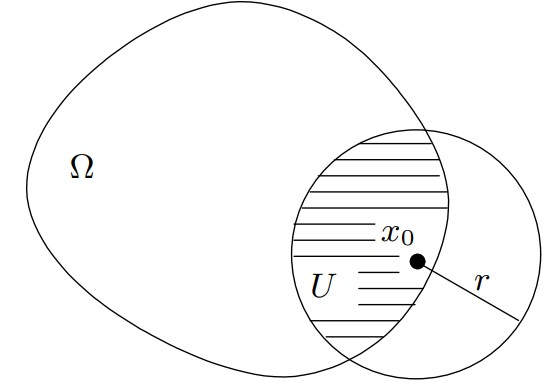
\includegraphics[width = 1\linewidth]{Bilder/Umgebung.jpg}
            \end{center}
        \end{minipage}
    \end{center}

    ii) Sei $E \subset \R^d$ offen. $U \subset \Omega$ heisst \textbf{relativ offen}, falls $U = E \cap \Omega$. \medskip

    iii) $A \subset \Omega$ heisst \textbf{relativ abgeschlossen}, falls $\Omega \setminus A$ relativ offen ist.




    \subsubsection{Satz: Weierstrass'sches Kriterium für Stetigkeit}
    % https://de.wikipedia.org/wiki/Stetige_Funktion#Stetigkeit_in_der_Topologie

    Sei $f: \Omega \subset \R^d \to \R^n$ und $x_0 \in \Omega$. Es sind äquivalent:

    \begin{center}
        \renewcommand{\arraystretch}{1.25}
        \begin{tabular}{r p{0.85\linewidth}} \toprule
                              & \hspace*{-10pt} $f$ ist an der Stelle $x_0$ stetig gemäss Folgekriterium.                                                                                              \\
            $\Leftrightarrow$ & \hspace*{-10pt} $\forall \epsilon > 0 \,\, \exists \delta > 0 \,\text{ s.d }\, \forall x \in \Omega: \, ||x - x_0|| < \delta \Rightarrow ||f(x) - f(x_0)|| < \epsilon$ \\
            $\Leftrightarrow$ & \hspace*{-10pt} Für jede Umgebung $V$ von $f(x_0)$ in $\R^n$ ist $U = f^{-1}(V)$ eine Umgebung von $x_0$ in $\Omega$.                                                  \\
            \bottomrule
        \end{tabular}
    \end{center}


    \subsubsection{Topologisches Kriterium für Stetigkeit}

    Für $f: \Omega \to \R^n$ sind äquivalent:

    \begin{center}
        \renewcommand{\arraystretch}{1.25}
        \eqboxf{\begin{tabular}{r p{0.8\linewidth}}
                                  & \hspace*{-10pt} $f$ ist stetig ($f \in C^0$).                                                                      \\

                $\Leftrightarrow$ & \hspace*{-10pt} Das Urbild $U = f^{-1}(V)$ jeder offenen Menge $V \subset \R^n$ ist relativ offen.                 \\
                $\Leftrightarrow$ & \hspace*{-10pt} Das Urbild $A = f^{-1}(B)$ jeder abgeschlossene Menge $B \subset \R^n$ ist  relativ abgeschlossen. \\
            \end{tabular}}
    \end{center}

    \begin{center}
        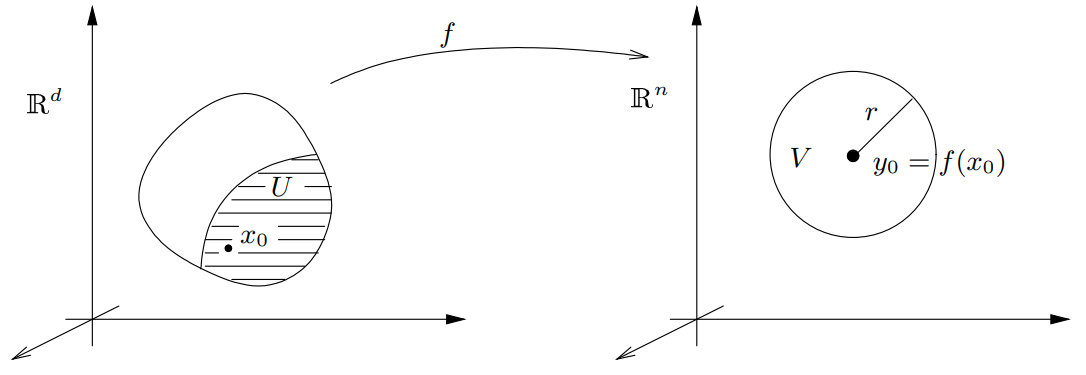
\includegraphics[width = 1\linewidth]{Bilder/TopoStetigkeit.png}
    \end{center}




    \section{Differentialrechnung auf $\R$}

    \subsection{Differential}

    Sei $f: \Omega \to \R$ mit $\Omega \subset \R$ offen und $x_0 \in \Omega$. $f$ heisst \emph{differenzierbar} an der Stelle $x_0$ falls folgender Grenzwert exisitert:

    \begin{center}
        \eqbox{$\dfrac{d f}{d x}(x_0) = f'(x_0) := \displaystyle \lim\limits_{h \to 0} \dfrac{f(x_0 + h) - f(x_0)}{h}$}
    \end{center}

    $f'(x)$ heisst \emph{Ableitung} (oder Differential) von $f$ an der Stelle $x_0$. \medskip

    Bemerkung: Analoges gilt für $f: \Omega \to \R^n$ (Vektorwertige Funktion), einfach Komponentenweise.

    \subsubsection{Geometrische Bedeutung}

    i) Der Differentialquotient $\frac{f(x) - f(x_0)}{x - x_0}$ entspricht der Steigung der Sekante durch die Punkte $(x,f(x)), (x_0, f(x_0))$. \medskip

    ii) Die Ableitung $f'(x_0)$ entspricht der Steigung der Tangente im Punkt $(x_0,f(x_0))$.

    \subsubsection{Satz}

    $f: \Omega \to \R$ differenzierbar an der Stelle $x_0 \in \Omega$ $\Rightarrow$ $f$ ist stetig in $x_0$.

    \subsubsection{Eigenschaften des Differentials}

    Seien $f,g: \Omega \to \R$ an der Stelle $x_0 \in \Omega$ differenzierbar. Dann gilt

    \begin{center}
        \renewcommand{\arraystretch}{1.75}
        \begin{tabular}{r l} \toprule
            Summenregel   & $(f(x_0) + g(x_0))' = f'(x_0) + g'(x_0)$                                                 \\
            Produktregel  & $(f(x_0) \cdot g(x_0))' = f'(x_0) g(x_0) + f(x_0)g'(x_0)$                                \\
            Quotientregel & $\left(\frac{f(x_0)}{g(x_0)}\right)' = \dfrac{f'(x_0) g(x_0) - g'(x_0)f(x_0)}{g^2(x_0)}$ \\
            Kettenregel   & $(g(x_0) \circ f(x_0))' = g'(f(x_0)) \cdot f'(x_0)$                                      \\ \bottomrule
        \end{tabular}
    \end{center}

    Bei der Quotientregel muss natürlich $g(x_0) \neq 0$ sein.


    \subsection{Der Mittelwertsatz}

    Seien $-\infty < a < b < \infty$. Sei $f:[a,b] \to \R$ stetig und differenzierbar in $]a,b[$. Dann existiert $x_0 \in ]a,b[$ mit

    \begin{center}
        $f(b) = f(a) + f'(x_0)(b - a)$ $\quad \Leftrightarrow \quad$ \eqboxf{$f'(x_0) = \dfrac{f(b) - f(a)}{b - a}$}
    \end{center}

    \subsubsection{Korollar}

    Sei $f:[a,b] \to \R$ stetig und differenzierbar auf $]a,b[$. Dann gilt:

    \begin{center}
        \renewcommand{\arraystretch}{1.25}
        \begin{tabular}{r l} \toprule
            i)   & Falls $f'(x) \equiv 0$ auf $]a,b[$, dann ist $f$ konstant           \\
            ii)  & Falls $f'(x) \geq 0$ auf $]a,b[$, dann ist $f$ monoton wachsend.    \\
            iii) & Falls $f'(x) > 0$ auf $]a,b[$, dann ist $f$ streng monton wachsend. \\
            \bottomrule
        \end{tabular}
    \end{center}

    \subsection{Der Umkehrsatz}

    Sei $f:]a,b[ \to \R$ differenzierbar mit $f'(x) > 0$ auf $]a,b[$. Seien

    \begin{center}
        $-\infty \leq c = \inf\limits_{a < x < b} f(x) < \sup\limits_{a < x < b} f(x) = d \leq \infty$
    \end{center}

    Dann ist $f:]a,b[\, \to \,]c,d[$ bijektiv und die Umkehrfunktion $f^{-1}:\,]c,d[\, \to \,]a,b[$ ist differenzierbar für $y \in ]c,d[$ und das Differential ist

    \begin{center}
        \eqboxf{$(f^{-1})' (y) = \dfrac{1}{f'(f^{-1}(y))}$}
    \end{center}


    \subsection{Funktionen der Klasse $C^1$}

    Sei $\Omega$ ein offenes Intervall und $f: \Omega \to \R$ differenzierbar. $f$ heisst von der Klasse $C^1(\Omega, \R)$, falls die Ableitung $f'(x)$ stetig ist. Es gilt also

    \begin{center}
        \eqbox{$C^1(\Omega, \R) = \{ f: \Omega \to \R; f, f' \text{ stetig} \}$}
    \end{center}

    \subsubsection{Satz}

    Sei $(f_k)_{k \in \mathbb{N}}$ eine Folge von Funktionen in $C^1(\Omega, \R)$ mit

    \begin{center}
        $f_k \xrightarrow[]{glm} f, f'_k \xrightarrow[]{glm} g \quad (k \to \infty)$
    \end{center}

    wobei $f, g: \Omega \to \R$. Dann gilt $f \in C^1(\Omega, \R)$ und $f' = g$.


    \subsection{Höhere Ableitungen}

    Sei $m \in \N$. $f$ heisst auf $\Omega$ m-Mal differenzierbar, falls die $m$-te Ableitung von $f$ existiert und wird folgendermassen notiert:

    \begin{center}
        $f^{(m)} = \dfrac{d^m f}{d x^m}$
    \end{center}

    \subsubsection{Funktionen der Klasse $C^m$}

    Sei $\Omega$ ein offenes Intervall und $f: \Omega \to \R^n$ $m$-Mal differenzierbar. $f$ heisst von der Klasse $C^m(\Omega, \R)$, falls $f^m(x)$ stetig ist. Es gilt also

    \begin{center}
        \eqbox{$C^m(\Omega, \R) = \{ f: \Omega \to \R; f \text{ ist \emph{m}-mal diffbar, } f, \dots, f^{(m)} \text{ stetig} \}$}
    \end{center}

    Bemerkung: Falls $f \in C^m(\Omega, \R)$ für alle $m \in \mathbb{N}$, dann schreibt man $f \in C^\infty(\Omega, \R)$. Solche Funktionen nennt man ''Glatte Funktionen''.




    \subsection{Taylor Entwicklung}
    %Mehr Infos: https://brilliant.org/wiki/taylor-series-error-bounds/

    %Gutes Bild: Vorlesung 27.04.23 @11min

    Sei $f \in C^{(m+1)}([a,b], \R)$ auf $]a,b[$ $m$-Mal differenzierbar. Die Taylorentwicklung $m$-ter Ordnung von $f$ am Entwicklungspunkt $a$ ist

    \begin{center}
        \eqboxf{$\displaystyle T_m f(x; a) = \sum\limits_{k = 0}^m f^{(k)} (a) \dfrac{(x - a)^k}{k!} + \underbrace{f^{(m+1)}(\xi) \dfrac{(x - a)^{m+1}}{(m+1)!}}_{\text{Restterm}}$}
    \end{center}

    Wobei $\xi \in \,]a,b[$ ist, d.h. eine beliebige Zahl im Definitionsbereich.

    \subsubsection{Beste Approximation}

    Je näher $x$ bei $a$ liegt, desto besser approximiert das Taylorpolynom $T_m f(x; a)$ an der Stelle $x$ die Funktion $f$. Für $a < x < b$ gilt

    \begin{center}
        \eqbox{$\lim\limits_{x \to a} \dfrac{f(x) - T_m f(x,a)}{(x - a)^m} = 0$}
    \end{center}

    \subsubsection{Abschätzung vom Restterm}

    Der Restterm $r_m f(x;a)$ besitzt folgende Abschätzung:

    \begin{center}
        \eqbox{$|r_mf(x,a)| \leq \sup\limits_{a < \xi < x} |f^{(m+1)}(\xi)| \dfrac{(x - a)^{m + 1}}{(m + 1)!}$}
    \end{center}


    \subsection{Lokale Extrema}

    Sei $\Omega \subset \R$ offen und $f: \Omega \to \R$. Ein $x_0 \in \Omega$ heisst (\emph{strikte}) lokale Minimalstelle von $f$, falls in einer Umgebung $U$ von $x_0$ gilt

    \begin{center}
        $f(x) \geq f(x_0), \, \forall x \in U$ \,\, (bzw. $f(x) > f(x_0), \, \forall x \in U\setminus \{x_0\}$)
    \end{center}

    Analoges gilt für lokale Maximastellen.

    \subsubsection{Satz}

    Sei $\Omega \subset \R$ offen, $f \in C^2(\Omega, \R)$ und $x_0 \in \Omega$. Es gilt folgendes:

    \begin{center}
        \renewcommand{\arraystretch}{1.25}
        \begin{tabular}{r l} \toprule
            i)   & Wenn $f'(x_0) = 0 \, \Rightarrow x_0$ ist ein lokales Extrema.                  \\
            ii)  & Sind $f'(x_0) = 0$ und $f''(x_0) > 0 \, \Rightarrow$ $x_0$ ein lokales Minimum. \\
            iii) & Sind $f'(x_0) = 0$ und $f''(x_0) < 0 \, \Rightarrow$ $x_0$ ein lokales Maximum. \\
            \bottomrule
        \end{tabular}
    \end{center}

    \textbf{Achtung}: Randpunkte vom Definitionsbereich nicht vergessen!

    \subsubsection{Allgemeinerer Satz}

    Sei $f \in \C^n(\Omega, \R)$ mit $f'(x_0) = \dots = f^{(n-1)}(x_0) = 0$ und $f^{(n)}(x_0) \neq 0$.

    \begin{center}
        \renewcommand{\arraystretch}{1.25}
        \begin{tabular}{r l} \toprule
            i)   & Ist $n$ gerade sowie $f^{(n)}(x_0) > 0$ $\,\Rightarrow$ $x_0$ ein lokales Minimum. \\
            ii)  & Ist $n$ gerade sowie $f^{(n)}(x_0) < 0$ $\,\Rightarrow$ $x_0$ ein lokales Maximum. \\
            iii) & Ist $n$ ungerade, so hat $f$ bei $x_0$ einen Wendepunkt.                           \\
            \bottomrule
        \end{tabular}
    \end{center}


    \subsection{Konvexe Funktionen}

    Sei $f \in C^2(]a,b[, \R)$ mit $f'' \geq 0$. Ein Funktion $f$ heisst \emph{konvex}, falls für alle $x_0, x_1 \in \, ]a,b[$ und für alle $t \in [0,1]$ gilt:

    \begin{center}
        \eqbox{$f(t \cdot x_1 + (1 - t)\cdot x_0) \leq t \cdot f(x_1) + (1 - t) \cdot f(x_0)$}
    \end{center}

    Die Funktionen für welche dies gilt heissen Konvex. \medskip

    Bemerkung: Wenn $f''(x) > 0$ $\Rightarrow$ $f(x)$ ist konvex.





    \section{Integralrechnung auf $\R$}


    \subsection{Stammfunktionen (SF)}

    $F \in C^1(]a,b[)$ heisst Stammfunktion zu $f$, falls für alle $x \in ]a,b[$ gilt:

    \begin{center}
        \eqbox{$\displaystyle \int f(x) dx = F(x)$ \qquad $F'(x) = f(x)$}
    \end{center}


    \subsubsection{Satz: Integrationskonstante}

    Zwei Stammfunktionen $F_1, F_2 \in C^1(]a,b[)$ einer Funktion unterscheiden sich nur durch eine Integrationskonstante voneinander: $F_1 - F_2 \equiv c \in \R$


    \subsubsection{Das Integral}

    Sei $F \in C^1(]a,b[,\R)$ eine SF von $f$. Das Integral von $f$ über $[a, b]$ ist:

    \begin{center}
        \eqbox{$\displaystyle \int\limits_{a}^b f(t) dt := F(b)-F(a)$}
    \end{center}


    \subsection{Eigenschaften vom Integral (und R-Integral)}

    \subsubsection{Linearität}

    Seien $f,g \in C^0(]a,b[)$ mit SFs $F,G \in C^1(]a,b[)$, und $\alpha, \beta \in \R$. Dann gilt

    \begin{center}
        \eqbox{$\displaystyle \int [\alpha \cdot f(x) + \beta \cdot g(x)] dx = \alpha \cdot \int f(x) dx + \beta \cdot \int  g(x) dx$}
    \end{center}


    \subsubsection{Monotonie}

    Seien $f,g \in C^0(]a,b[)$ mit SFs $F,G \in C^1(]a,b[)$, und $f \leq g$. Dann gilt

    \begin{center}
        \eqbox{$\displaystyle \int\limits_{x_0}^{x_1} f(t) dt \leq \int\limits_{x_0}^{x_1} g(t) dt$}
    \end{center}


    \subsubsection{Gebietsadditivität}

    Sei $f \in C^0(]a,b[)$ mit SF $F \in C^1(]a,b[)$. Für $a < x_0 \leq x_1 \leq x_2 < b$ gilt:

    \begin{center}
        \eqbox{$\displaystyle \int\limits_{x_0}^{x_1} f(x) dx + \int\limits_{x_1}^{x_2} f(x) dx = \int\limits_{x_0}^{x_2} f(x) dx$}
    \end{center}

    \subsubsection{Standardabschätzung}

    Sei $f \in C^0([a,b])$. Dann gilt folgende Abschätzung

    \begin{center}
        \eqbox{$\displaystyle \left| \int\limits_a^b f(x) dx \right| \leq \int\limits_a^b |f(x)| dx \leq ||f(x)||_{C^0} (b - a)$}
    \end{center}

    \subsubsection{Korollar bezüglich glm. Konveregenz}

    Seien $f, f_k \in C^0([a,b])$ mit $f_k \xrightarrow[]{glm} f \, (k \to \infty)$. Dann gilt

    \begin{center}
        \eqbox{\hspace*{-5pt}$\displaystyle \left| \int\limits_a^b f_k dx - \int\limits_a^b f dx \right| \leq \int\limits_a^b |f_k - f| dx \leq (b - a) \, || f_k - f||_{C^0} \to 0 (k \to \infty)$\hspace*{-5pt}}
    \end{center}




    \subsection{Treppenfunktionen}

    $f: [a,b] \to \R$ heisst Treppenfunktion, falls für eine Zerlegung $I = [a,b]$ in disjunkte (abgeschlossene, offene, halboffene) Teilintervalle $I_1, \dots, I_K$ mit dazugehörigen \emph{Konstanten} $c_k \in \R$ gilt:


    \begin{minipage}{0.74\linewidth}
        \begin{center}
            \eqbox{$\displaystyle f(x) = \sum\limits_{k = 1}^K c_k \cdot \chi_{I_k}$ mit $\chi_{I_k}(x) = \begin{cases}
                        1 & , x \in I_k \\ 0 & , x \not\in I_k \\
                    \end{cases}$}
        \end{center}
    \end{minipage}
    \begin{minipage}{0.25\linewidth}
        \begin{center}
            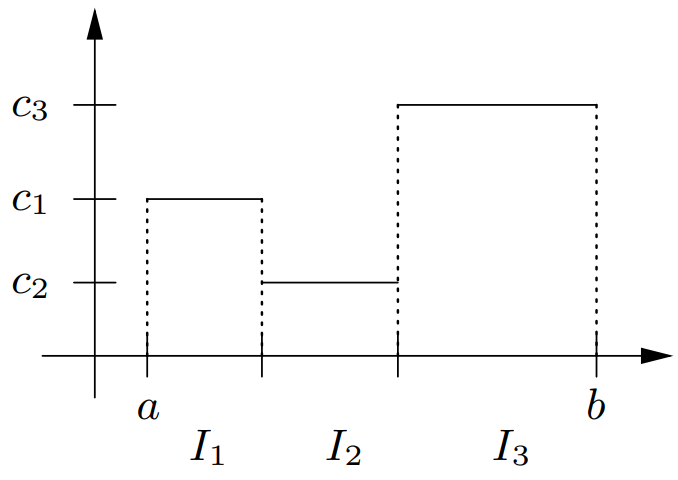
\includegraphics[width=1\linewidth]{Bilder/RiemannSumme.png}
        \end{center}
    \end{minipage}



    Sei $|I_k|$ die Länge von $I_k$. Das Integral einer Treppenfunktion $f(x)$ ist

    \begin{center}
        \eqbox{$\displaystyle \int\limits_{a}^{b} \left(\sum\limits_{k = 1}^K c_k \cdot \chi_{I_k}\right) dx = \sum\limits_{k = 1}^K c_k \cdot |I_k|$}
    \end{center}

    \subsubsection{Lemma}

    Sind $e,g:[a,b] \to \R$ Treppenfunktionen mit $e \leq g$, dann gilt

    \begin{center}
        $\int\limits_a^b e(x) dx \leq \int\limits_a^b g(x) dx$
    \end{center}


    \subsection{Die Riemannsche Summe}

    Sei $f\in C^0([a,b])$. Dann gilt für eine beliebige Folge von disjunkte Zerlegung von $I$ in Teilintervalle $I_k^n, 1 \leq k \leq K_n$ mit \emph{Feinheit}

    \begin{center}
        $\delta_n = \sup\limits_{1 \leq k \leq K_n} |I_k^n| \to 0 \quad (n \to \infty)$
    \end{center}

    und eine beliebigen Auswahl an Punkten $x_k^n \in I^n_k, \, 1 \leq k \leq K_n$, stets

    \begin{center}
        \eqbox{$\displaystyle\int\limits_a^b \left( \sum\limits_{k = 1}^{K_n} f(x_k^n) \chi_{I_k^n}\right) dx = \sum\limits_{k = 1}^{K_n} f(x_k^n) | I_k^n | \to \int\limits_a^b f(x) dx \, (n \to \infty)$}
    \end{center}


    \subsection{Das Riemannsche Integral (R-Integral)}

    Sei $f:[a,b] \to \R$ beschränkt und seien $e(x),g(x)$ Treppenfunktionen.

    \begin{center}
        Untere Riemann-Integral von $f$: \, \eqbox{$\displaystyle \underline{\int\limits_{a}^b} f(x) dx = \sup\limits_{e(x) \leq f(x)} \int\limits_a^b e(x) dx$} \medskip

        Obere Riemann-Integral von $f$: \eqbox{$\displaystyle \overline{\int\limits_a^b} f(x) dx = \inf\limits_{g(x) \geq f(x)} \int\limits_a^b g(x) dx$}
    \end{center}

    Ein solches $f(x)$ heisst über $[a,b]$ Riemann-integrabel, falls

    \begin{minipage}{0.3\linewidth}
        \begin{center}
            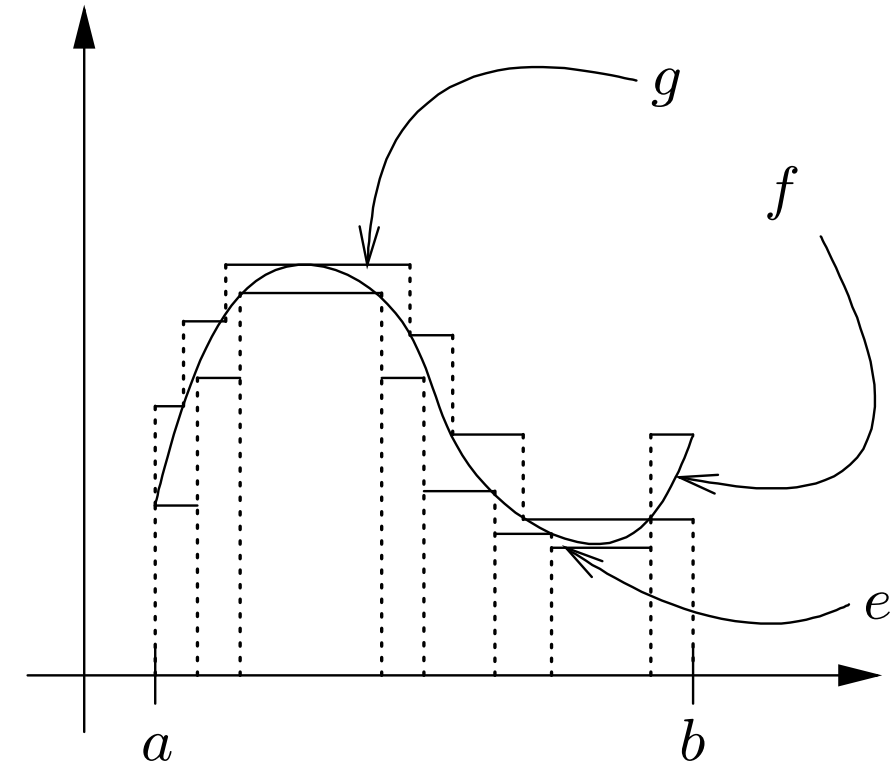
\includegraphics[width=0.8\linewidth]{Bilder/R-Integral.png}
        \end{center}
    \end{minipage}
    \begin{minipage}{0.69\linewidth}
        \begin{center}
            \eqbox{$\displaystyle \underline{\int\limits_{a}^b} f(x) dx = \overline{\int\limits_a^b} f(x) dx := \int\limits_a^b f(x) dx$}
        \end{center}
    \end{minipage}

    \subsubsection{Sätze}

    i) $f:[a,b] \to \R$ monoton, beschränkt $\Rightarrow f$ ist über $[a,b]$ R-integrabel. \medskip

    ii) $f:[a,b] \to \R$ stetig ($f \in C^0([a,b], \R)$) $\Rightarrow f$ ist über $[a,b]$ R-integrabel.




    \subsection{Substitutionsregel}

    Seien $f,g \in C^1(]a,b[)$. Dann gilt für $a < x_0 < x_1 < b$:

    \begin{center}
        \eqboxf{$\displaystyle \int\limits_{x_0}^{x_1} f'(\underbrace{g(x)}_{= u}) \cdot \underbrace{g'(x) dx}_{= d u} = \int\limits_{g(x_0)}^{g(x_1)} f'(u) du$}
    \end{center}


    \subsection{Partielle Integration}

    Seien $u,v \in C^1(]a,b[)$, so dass $u(x) \cdot v'(x)$ eine SF besitzt. Dann besitzt $u'(x) \cdot v(x)$ auch eine SF und es gilt

    \begin{center}
        \eqboxf{$\displaystyle \int\limits_a^b u'(x) v(x) dx = [u(x)v(x)]_a^b - \int\limits_a^b u(x) v'(x) dx $}
    \end{center}

    \subsubsection{Bei periodischen Funktion}

    Bei Partieller Integration von zwei periodischen Funktionen geht man eine Periode durch und sotiert dann das ''ursprüngliche Integral'' auf die Linke Seite und kann so, dass Integral berechnen.


    \subsection{Hauptsatz der Differential- und Integralrechnung}

    Sei $f \in C^0([a,b], \R)$. So ist für jedes $c \in [a,b]$ die Integralfunktion

    \begin{center}
        \eqbox{$\displaystyle F: [a,b] \to \R$ mit $\displaystyle F(x) = \int\limits_c^x f(t) dt$}
    \end{center}

    differenzierbar und es gilt für alle $x \in [a,b]$: $F'(x) = f(x)$.

    \subsubsection{Anwendung: Parameterintegral}

    \begin{center}
        $\displaystyle \frac{d}{dt} \int\limits_a^{h(t)} g(x) dx = \frac{d}{dt} [G(x)]^{h(t)}_{a} = g(h(t)) \cdot h'(t)$
    \end{center}


    \subsection{Uneigentliches Riemann-Integral}

    Sei $f: ]a,b[ \to \R$ mit $-\infty \leq a < b \leq \infty$ über jedes kompakte Intervall $[c,d] \subset ]a,b[$ R-integrabel. $f$ ist über $]a,b[$ \emph{uneigentlich R-integrabel}, falls folgender Grenzwert existiert:

    \begin{center}
        \eqbox{$\displaystyle \int\limits_{a}^b f(x) dx = \lim\limits_{c \to a^+} \int\limits_{c}^0 f(x) dx + \lim\limits_{d \to b^-} \int\limits_{0}^d f(x) dx$}
    \end{center}

    \subsubsection{Satz: Reihenkonvergenz}

    Sei $f:[1, \infty) \to \R_+$ \emph{monoton fallend}. Dann gilt

    \begin{center}
        \eqbox{$\displaystyle \sum\limits_{k = 1}^\infty f(x)$ konvergiert $\Leftrightarrow$ $\displaystyle \int\limits_1^\infty f(x) dx$ konvergiert}
    \end{center}

    \section{Gewöhnliche lineare Differentialgleichungen (GDG)}


    \subsection{Differentialgleichungen 1ter Ordnung}

    \subsubsection{Homogene Lösung}

    Die Homogene Differentialgleichung 1ter Ordnung hat die Form:

    \begin{center}
        \eqbox{$y'(x) - a(x) y(x) = 0$}
    \end{center}

    Den Lösungsansatz nennt man \emph{Seperation der Variablen}:

    \begin{center}
        \renewcommand{\arraystretch}{1.5}
        \begin{tabular}{r p{0.8\linewidth}} \toprule
            i)   & $y'(x) - a(x) y(x) = 0 \Leftrightarrow \dfrac{d y}{d x} = a(x) y(x)$                     \\
            ii)  & Umformen auf folgende Form:

            \begin{center}
                $\frac{1}{y(x)} dy = a(x) dx$
            \end{center}                                                           \\
            iii) & Auf beiden Seiten integrieren:

            \begin{center}
                $\displaystyle \int \frac{1}{y(x)} dy = \int a(x) dx \Rightarrow \log(y(x)) = A(x) + C$
            \end{center} \\
            iv)  & Auf beide Seiten $e^x$ anwenden:

            \begin{center}
                \eqboxf{$y_h(x) = e^{A(x)} \cdot C$}
            \end{center}                                       \\
            \bottomrule
        \end{tabular}
    \end{center}

    Bemerkung: $A(x)$ ist die SF von $a(x)$ und $C$ die Integrationskonstante.


    \subsubsection{Inhomogene Differentialgleichungen 1ter Ordnung}

    Eine Inhomogene Differentialgleichung 1ter Ordnung hat die Form:

    \begin{center}
        \eqbox{$y'(x) - a(x) y(x) = b(x)$}
    \end{center}

    Den Lösungsansatz nennt man \emph{Variation der Konstanten}:

    \begin{center}
        \renewcommand{\arraystretch}{1.5}
        \begin{tabular}{r p{0.8\linewidth}} \toprule
            i)   & Die homogene Lösung $y'(x) - a(x) y(x) = 0$ berechnen.                                                                  \\
            ii)  & Man macht den Ansatz, dass $C$ von $x$ abhängt:

            \begin{center}
                $y_h(x) = C(x) \cdot e^{A(x)}$
            \end{center}                                                                            \\
            iii) & Man berechnet $y_h'(x)$:

            \begin{center}
                $y_h'(x) = C'(x)e^{A(x)} + C(x) a(x) e^{A(x)}$
            \end{center}                                      \\
            iv)  & $y_h'(x)$ und $y_h(x)$ in die ursprüngliche DGL einsetzen:

            \begin{center}
                $C'(x)e^{A(x)} \underbrace{+ C(x) a(x) e^{A(x)} - C(x) a(x) e^{A(x)}}_{= 0} = b(x)$
            \end{center}                                                            \\
            v)   & Gleichung umstellen und dann Integrieren:

            \begin{center}
                $\displaystyle C'(x) = \dfrac{b(x)}{e^{A(x)}} \Rightarrow C(x) = \int \dfrac{b(x)}{e^{A(x)}} dx + K$
            \end{center}                          \\
            vi)  & Gefundes $C(x)$ in $y_h(x) = C(x) \cdot e^{A(x)}$ einsetzen, dies ist die Lösung der inhomogenen Differentialgleichung.
            \\
            \bottomrule
        \end{tabular}
    \end{center}
    \subsubsection*{DGL n-ter Ordnung}
    Eine lineare DGL der n-ten Ordnung hat folgende Form
    \begin{equation*}
        a_0y^{(0)}+\dots+ a_ny^{(n)}=q(x)
    \end{equation*}
    \begin{annotation}{Anmerkung}
        \item [i)]  $q(x)$ bezeichnet die Inhomogenität
        \item [ii)] Da die DGL linear ist, gilt für die Lösung
        \begin{equation*}
            y(x)=y_h(x)+y_p(x)
        \end{equation*}
        wobei $y_h$ die homogene und $y_p$ die partikuläre Lösung ist
    \end{annotation}
    \subsubsection{Homogene Lösung $(q(x)=0)$}
    \begin{enumerate}
        \item Man setzt die Inhomogenität 0
              \begin{equation*}
                  a_0y^{(0)}+\dots+ a_ny^{(n)}=0
              \end{equation*}
        \item Mit dem Ansatz $y(x)=e^{\lambda x}$ folgt das charakteristische Polynom
              \begin{equation*}
                  \text{Chp}(\lambda)=a_0\lambda^0+a_1\lambda^1+\dots +a_n\lambda^n=0
              \end{equation*}
        \item Nullstellen in den Ansatz einsetzen
              \begin{itemize}
                  \item $\lambda_i$  k-fache reelle Nullstelle
                        \begin{equation*}
                            y_i(x)=x^0e^{\lambda_i x}, \dots,~ y_{i+k}(x)=x^{k-1}e^{\lambda_i x}
                        \end{equation*}
                  \item $\lambda_i$ und $\lambda_j$ reelle betragsmässig gleiche Nullstelle ($\lambda = \pm a$)
                        \begin{equation*}
                            y_{i}(x) = \cosh(ax), ~y_j(x)=\sinh(ax)
                        \end{equation*}
                  \item $\lambda_i$ und $\lambda_j$ komplexe Nullstelle ($\lambda = a \pm bi$)
                        \begin{equation*}
                            y_{i}(x)=e^{ax}\cos(bx), ~y_j(x)=e^{ax}\sin(bx)
                        \end{equation*}
              \end{itemize}
        \item Die einzelnen Teillösungen zusammensetzen ($C_i \in \mathbb{R}$)
              \begin{equation*}
                  y_h(x)=\sum_{i=1}^{n}C_i y_i(x)
              \end{equation*}
    \end{enumerate}
    \subsubsection{Allgemeines Vorgehen zur Berechnung der partikulären Lösung}

    Die partikuläre Lösung $F_{part}(t) \in C^1(\R,\R^n)$ löst folgende Gleichung:

    \begin{center}
        \eqbox{$\dot F_{part} = A F_{part} (t) + B(t)$ \qquad bzw. $f^{(n)} + \dots + a_0 f = b(t)$}
    \end{center}

    Das Vorgehen ist, wie folgt:

    \begin{center}
        \begin{tabular}{r p{0.8\linewidth}} \toprule
            i)   & Den der Störfunktion $b(t)$ entsprechenden Ansatz suchen.                         \\
            ii)  & Ableitungen des Ansatzes $f_{part}$ berechnen.                                    \\
            iii) & $f_{part}$ mit ihren Ableitungen in die GDG einsetzen.                            \\
            iv)  & Die Koeffizienten vom Lösungsansatz durch einen Koeffizientenvergleich bestimmen. \\
            \bottomrule
        \end{tabular}
    \end{center}

    \begin{center}
        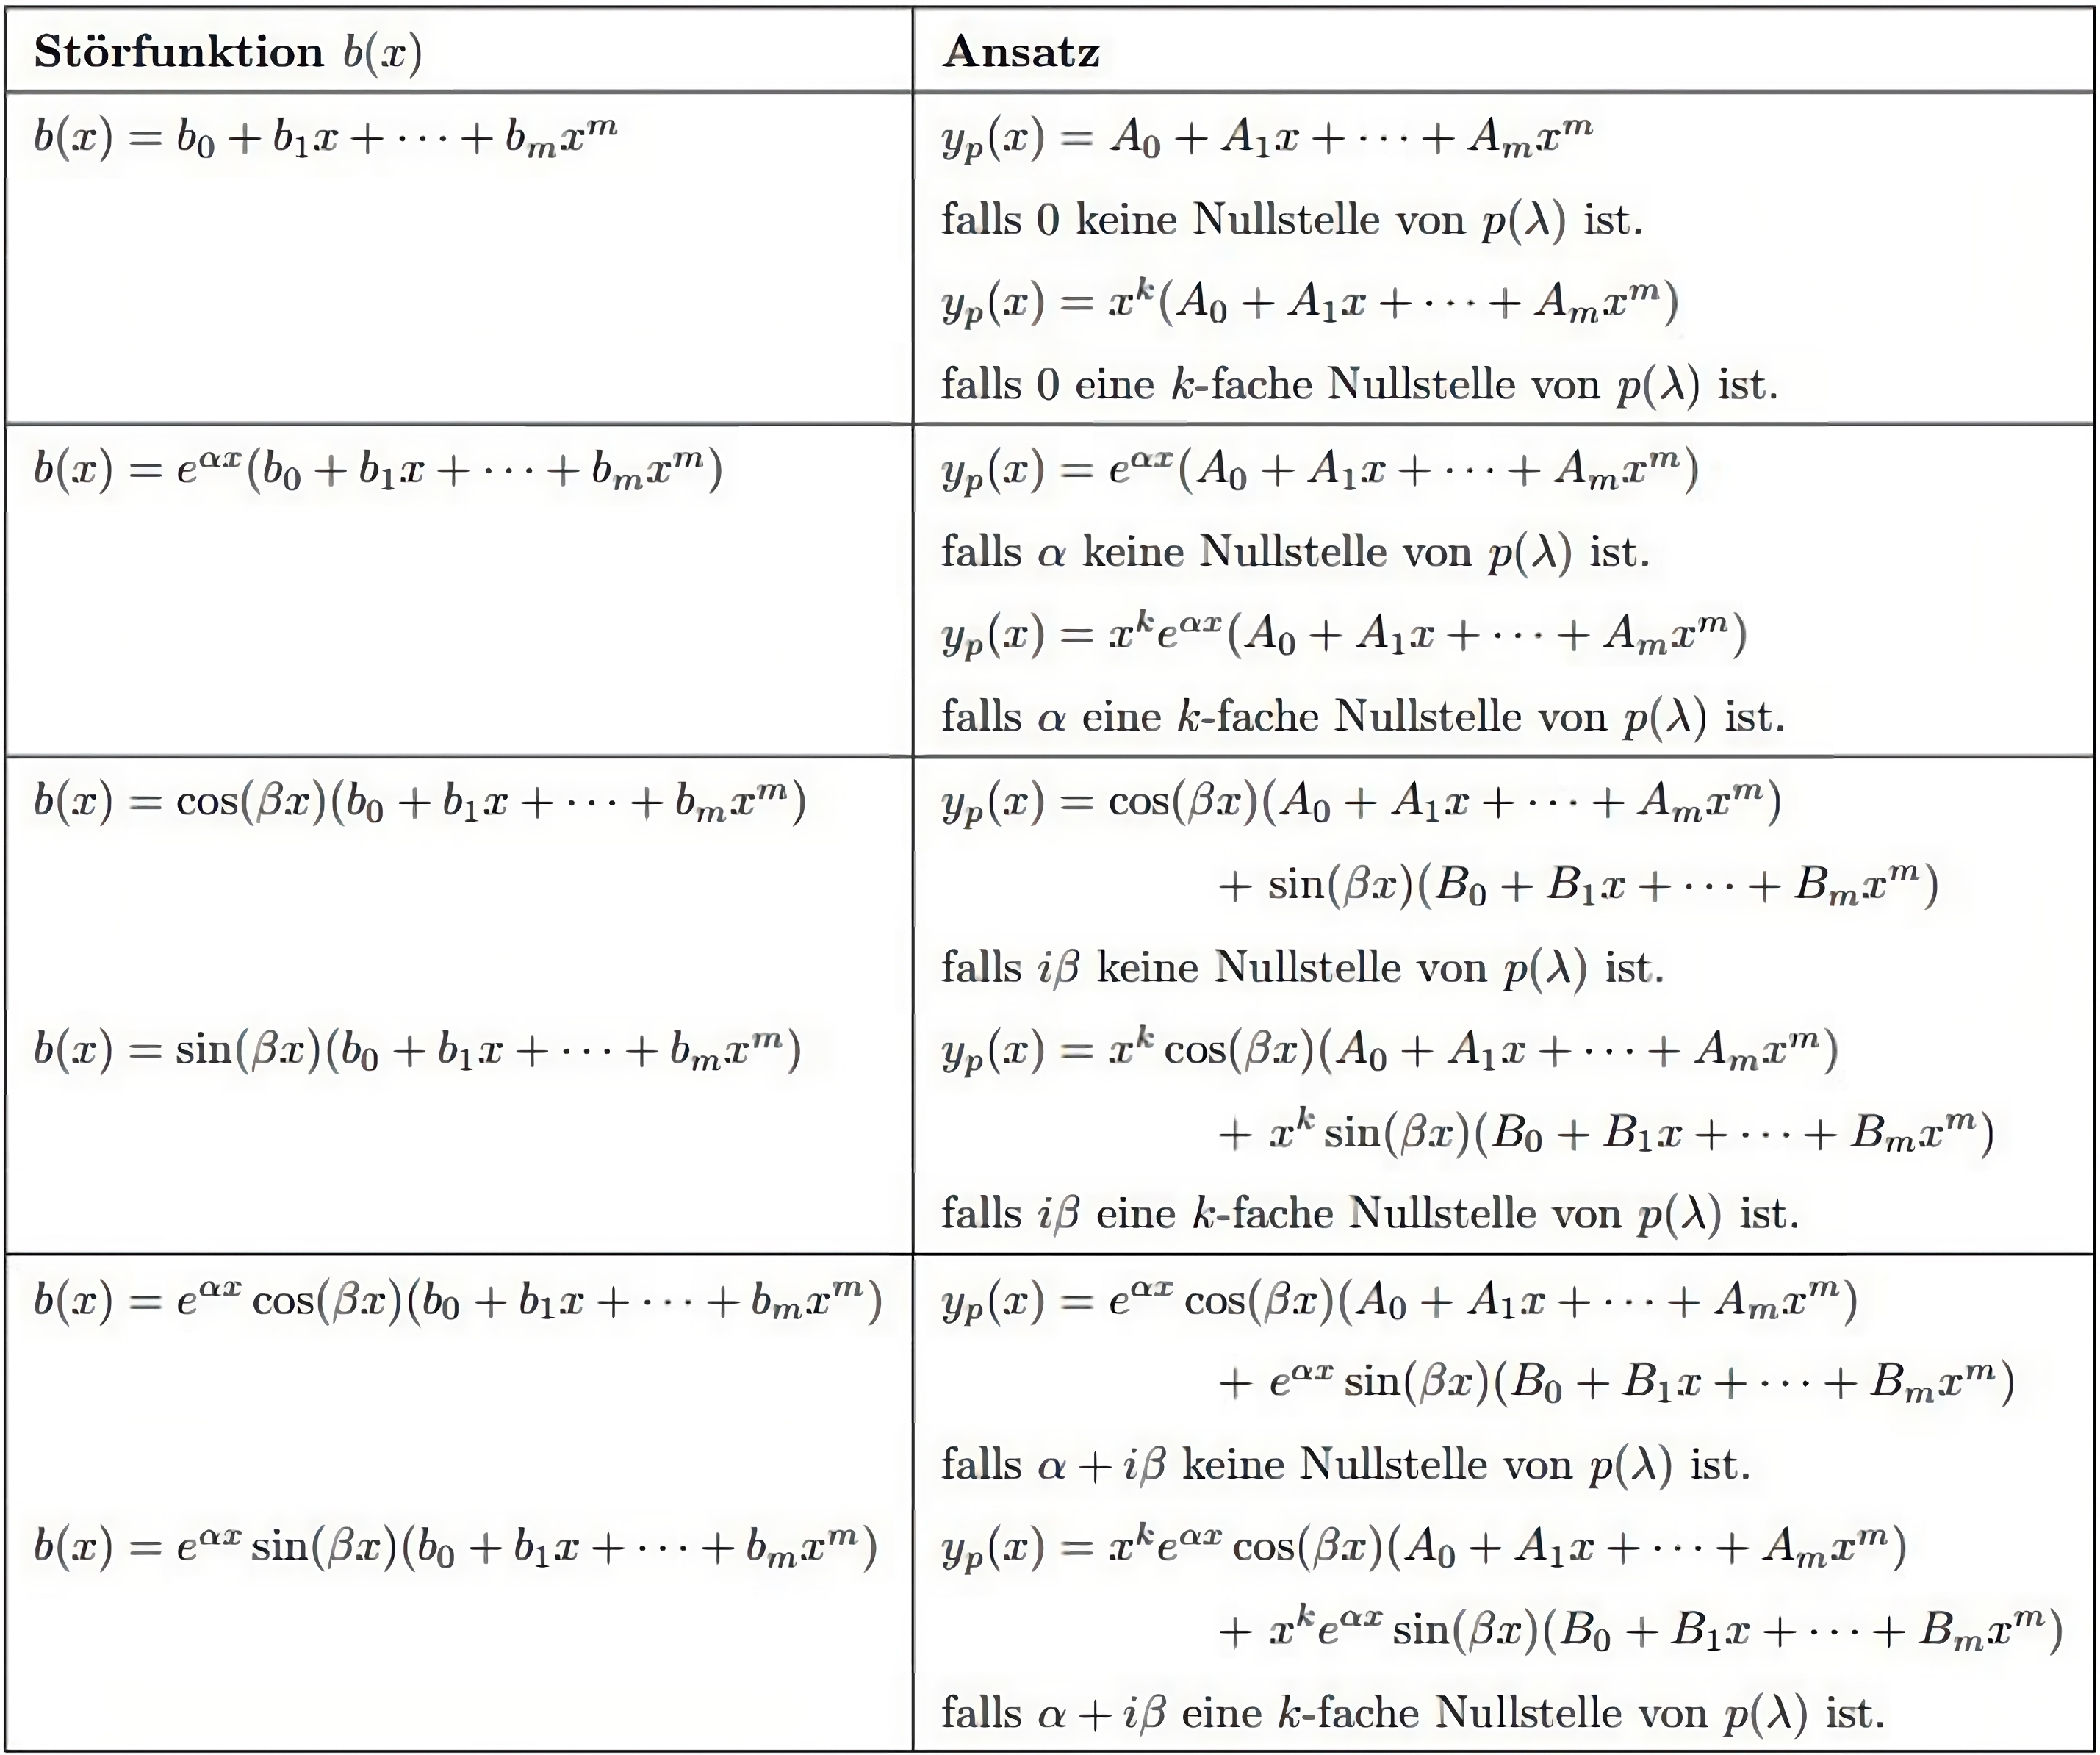
\includegraphics[width = 1\linewidth]{Bilder/DGL_Partikulare.jpeg}
    \end{center}
    \subsection{Homogene Systeme linearer Differentialgleichungen}
    Wenn wir einen Vektor $F(t) \in \R^n$ von Funktionen betrachten, kann folgende DGL 1. Ordnung betrachtet werden:
    \begin{center}
        \eqbox{$\dfrac{d F(t)}{d t} = A \cdot F(t)$}
    \end{center}

    Die Loesung des Anfangswertproblems $F(0) = F_0$ ist gegeben durch:

    \begin{center}
        \eqbox{$\dfrac{d F}{d t} = A \cdot F(t), \quad F(0) = F_0$}
    \end{center}

    diese besitzt \emph{genau} eine Lösung $F \in C^1(\R; \R^n)$.


    \subsubsection{Die Fundamentallösung}

    Folgende Matrix-wertige Funktion $\Phi(t) \in C^1(\R, M_{n \times n} (\R))$

    \begin{center}
        \eqbox{$t \mapsto \Phi(t) := Exp(A t) = \sum\limits_{k = 0}^\infty \dfrac{A^k t^k}{k!}$}
    \end{center}

    besitzt die erwünschten Eigenschaften

    \begin{center}
        $\dfrac{d\Phi}{d} = A \cdot \Phi(t), \, \Phi(0) = id$
    \end{center}

    Sie heisst Fundamentallösung von dem System $\dot F = A F(t)$. \\

    \subsubsection*{Matrixexponential}
    Das Matrixexponential einer $nxn$ Matrix $A$ ist definiert als:
    \begin{equation*}
        e^{At}=\sum_{k=0}^{\infty}\frac{A^kt^k}{k!}
    \end{equation*}
    Loesungsarten:
    \begin{itemize}
        \item \textbf{Nilpotente Matrix} ($A^n=0$, $n\in \mathbb{N}$): \\
              Berechnung folgt direkt aus der Definition des Matrixexponentials.
        \item \textbf{Diagonalmatrix}
              Exponentialfunktion kann auf alle Diagonalelemente einzeln angewendet werden.
        \item \textbf{Diagonalisierbare Matrix} ($A$ ist ähnlich zu einer Diagonalmatrix): \\
              Sei $A = T \begin{pmatrix}
                      \lambda_1 &        & 0         \\
                                & \ddots &           \\
                      0         &        & \lambda_n \\
                  \end{pmatrix} T^{-1}$, wobei $T$ die $n$ Eigenvektoren von $A$ als Spaltenvektoren enthält. \\
              Die Fundamentallösung nimmt folgende Form an:
              \begin{equation*}
                  \Phi(t) = Exp(t A) = T \begin{pmatrix}
                      e^{t \lambda_1} &        & 0               \\
                                      & \ddots &                 \\
                      0               &        & e^{t \lambda_n} \\
                  \end{pmatrix} T^{-1}
              \end{equation*}
    \end{itemize}

    \subsection{Reduktion der Ordnung}

    Die Allgemeine Form einer DGL n-ter Ordnung ist:

    \begin{center}
        \eqbox{$f^{(n)} + a_{n-1} f^{(n-1)} + \dots +a_1 \dot f + a_0 f = 0$}
    \end{center}

    Die Reduktion zu einem System 1.Ordnung ist:

    \begin{center}
        $\underbrace{\begin{pmatrix}
                    \dot f \\ \ddot f \\ \vdots \\ f^{(n)} \\
                \end{pmatrix}}_{\dot F} = \underbrace{\begin{bmatrix}
                    0      & 1    &        & 0        \\
                    \vdots &      & \ddots &          \\
                    0      & 0    &        & 1 \quad  \\
                    -a_0   & -a_1 & \dots  & -a_{n-1} \\
                \end{bmatrix}}_{A_{n \times n}} \underbrace{\begin{pmatrix}
                    f \\ \dot f \\ \vdots \\ f^{(n-1)} \\
                \end{pmatrix}}_{F(t)}$
    \end{center}

    \subsection{Der Lösungsraum}

    Sei $A \in M_{n \times n}(\R)$. Der Lösungsraum

    \begin{center}
        \eqbox{$X_A = \{F \in C^1(\R, \R^n) ; \, \dot F = A F\}$}
    \end{center}

    bildet ein $n$-dimensionaler $\R$-Vektorraum (Unterraum von $C^1(\R, \R^n)$). \medskip

    Analoges gilt für $A \in M_{n \times n}(\C)$:

    \begin{center}
        $\tilde{X}_A = \{F \in C^1(\R, \C^n) ; \, \dot F = A F\}$
    \end{center}

    bildet ein $n$-dimensionaler $\C$-Vektorraum.

    \subsubsection{Korollar}

    Sei $a = \{a_0, a_1, \dots, a_{n-1}\} \in \R$ (oder $\C$). Der Lösungsraum

    \begin{center}
        $Z_a = \{f \in C^n (\R, \R^n) ; \, f^{(n)} + a_{n-1} f^{(n-1)} + \dots + a_0 f = 0\}$
    \end{center}

    ist ein $n$-dimensionaler Unterraum von $C^n(\R, \R^n)$.


    \subsection{Einschub: Der Fundamentalsatz der Algebra}

    Sei $\lambda_i \in \mathbb{C}$ und $m_i \in \mathbb{N}$. Ein Polynom besitzt $n$ Nullstellen in $\C$, d.h.:

    \begin{center}
        $\displaystyle p(\lambda) = \prod\limits_{i = 1}^{l} (\lambda - \lambda_i)^{m_i}$ \qquad wobei \,\, $\displaystyle \sum\limits_{i = 1}^l m_i = n$
    \end{center}

    wobei $\lambda_i$ die Nullstellen mit jeweiliger Vielfachheit $m_i$ sind.


    \subsection{Inhomogene Differentialgleichungen höherer Ordnung}

    Seien $A \in M_{n \times n}(\R)$ und $B \in C^{0}(\R, \R^n)$. Sei $F_{part} \in C^1(\R,\R^n)$ eine beliebige ''\emph{partikuläre}'' Lösung von

    \begin{center}
        \eqbox{$\dot F = A F(t) + B(t)$}
    \end{center}

    Dann ist jede dazugehörige Lösung $F$ von der Form

    \begin{center}
        \eqboxf{$F(t) = F_{part}(t) + F_{hom} (t)$}
    \end{center}

    wobei $F_{hom}$ eine Lösung der homogenen Gleichung $\dot F = A F(t)$ ist. \medskip

    Eindeutigkeitssatz: Insbesondere gibt es zu jedem $F_0 \in \R^n$ stets genau eine Lösung $F(t)$ mit $F(0) = F_0$.

    \subsection{Sonstiges}

    \subsubsection{Harmonische Oszillatoren}

    Harmonische Oszillatoren besitzen folgende DGL:

    \begin{center}
        $\ddot f + \omega_0^2 f = 0, \, \omega^2_0 > 0 \quad \Rightarrow p(\lambda) = \lambda^2 + \omega_0 = 0 \quad \Rightarrow \lambda_1,2 = \pm i \omega_0$
    \end{center}

    Die Allgemeine Lösung hat, unter anderem, folgende Formen:

    \begin{center}
        $f(t) = A e^{i \omega_0 t} + B e^{-i \omega_0 t}$ \qquad $f(t) = A \cos(\omega_0 t) + B \sin(\omega_0 t)$
    \end{center}

    Die Reelle Lösung (Physikalische) bildet man durch die Summe und Differenz der ersten Lösung unter Anwendung der Eulerschen Formel (Koeffizienten A,B erst am Schluss anfügen).


    \subsubsection{Erzwungene Schwingungen}

    Die folgende DGL einer erzwungene Schwingung wandelt man, wie folgt, zur Berechnung der partikulären:

    \begin{center}
        $\ddot f + 2\delta \dot f + \omega_0^2 f = \beta_0 \cos(\omega t) \quad \Rightarrow \ddot f + 2\delta \dot f + \omega_0^2 f = \beta_0 e^{i\omega t}$
    \end{center}

    Benutzt man den Ansatz $f_{part} = c \cdot e^{i \omega t}$. So bekommt man:

    \begin{center}
        $c = \dfrac{\beta_0}{(\omega_0^2 - \omega^2) + 2 i \delta \omega} = \beta_0 \dfrac{\omega_0^2 - \omega^2 - 2i \delta \omega}{(\omega_0^2 - \omega^2)^2 + 4 \delta^2 \omega^2}$
    \end{center}

    Drückt man dies in der Polarform $R \cdot e^{i \varphi}$ aus:

    \begin{center}
        $R = \dfrac{\beta_0}{\sqrt{(\omega_0^2 - \omega^2)^2 + 4 \delta^2 \omega^2}}$ \qquad $\varphi = \arctan\left( \dfrac{-2 \delta \omega}{\omega_0^2 - \omega^2} \right) \in \, ]-\pi,0[$
    \end{center}

    Und setzt $c$ wieder ein in $f_{part}$:

    \begin{center}
        $f_{part} = c \cdot e^{i \omega t} = R \cdot e^{i(\omega t + \varphi)}$
    \end{center}

    Nun kann man noch den Realteil nehmen und hat dann die gesuchte partikuläre Lösung:

    \begin{center}
        $\tilde{f}_{part}(t) = \Re{f_{part}(t)} = R \cdot \cos(\omega t + \varphi)$
    \end{center}



    \section{Differentialrechnung in $\R^n$}

    \subsection{Partielle Ableitung}

    Sei $\Omega \subset \R^n$ offen. $f: \Omega \to \R$ heisst in $x_0$ in Richtung $e_i = (0, \dots, 1, \dots 0)$ partiell differenzierbar, falls folgender Grenzwert exisitert:

    \begin{center}
        \eqboxf{$\dfrac{\partial f}{\partial x^i} (x_0) = \partial_{x^i} f (x_0) = \lim\limits_{h \to 0} \dfrac{f(x_0 + h \cdot e_i) - f(x_0)}{h}$}
    \end{center}

    \begin{center}
        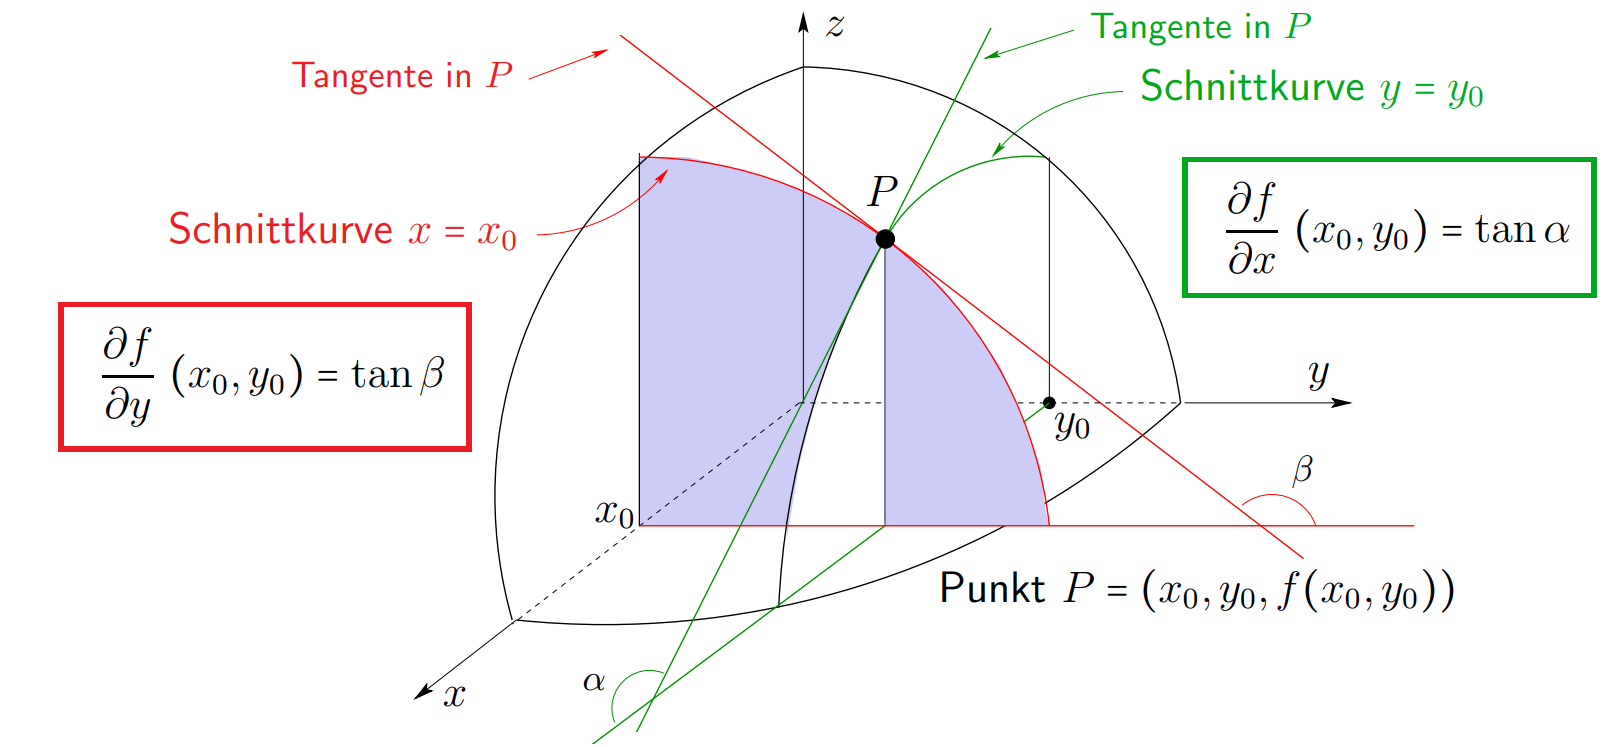
\includegraphics[width = 1\linewidth]{Bilder/PartiellAbleitung.png}
    \end{center}


    \subsubsection{Tangentialebene}
    %https://de.wikipedia.org/wiki/Tangentialebene#Tangentialebene_an_den_Graphen_einer_Funktion

    Die Tangentialebene ist die beste Approximation einer 2D-Funktion in der Nähe von $(x_0, y_0)$. Sie ist, wie folgt, definiert:

    \begin{center}
        \eqbox{$g(x,y) = f(x_0,y_0) + \dfrac{\partial f}{\partial x}(x_0,y_0) \cdot (x - x_0) + \dfrac{\partial f}{\partial y}(x_0,y_0) \cdot (y - y_0)$}
    \end{center}


    \subsection{Differential}

    Sei $\Omega \subset \R^n$ offen. $f: \Omega \to \R$ heisst differenzierbar an der Stelle $x_0$, falls eine lineare Abbildung $A: \R^n \to \R$ existiert mit

    \begin{center}
        \eqbox{$\lim\limits_{x \to x_0} \dfrac{f(x) - f(x_0) - A \cdot (x - x_0)}{|| x - x_0||} = 0$}
    \end{center}

    Dann heisst $d f_{x_0} := A$ (ein sogenannter co-Vektor) das Differential von $f$ an der Stelle $x_0$ und desweiteren gilt

    \begin{center}
        $d f_{x_0} \cdot (x - x_0) = \begin{bmatrix}
                \dfrac{\partial f}{\partial x^{0}} (x_0), \dots, \dfrac{\partial f}{\partial x^{n}} (x_0) \\
            \end{bmatrix} \begin{pmatrix}
                x^1 - x_0^1 \\ \vdots \\ x^n - x^n_0 \\
            \end{pmatrix}$
    \end{center}

    \begin{annotation}{Anmerkung}
        \item[i)] Bem: $dx^{i} = (0, \dots, 0, 1, 0, \dots 0)$ sind die Basiselemente von $d f_{x_0}$.
        \item [ii)]  Die Matrix $A$ ist die Jacobi-Matrix von $f$.
    \end{annotation}

    \subsubsection*{Jacobi-Matrix (Ableitungsmatrix)}
    Das Differential mit Einheitsvektoren heisst \emph{Jacobi-Matrix} ($M_{l \times n} (\R)$):

    \begin{center}
        \eqboxf{$df_{(x_0)} = \begin{pmatrix}
                    df^1_{(x_0)} \\ \vdots \\ df^l_{(x_0)}
                \end{pmatrix} =  \begin{pmatrix}
                    \frac{\partial f^1}{\partial x_1} & \dots  & \frac{\partial f^1}{\partial x_n} \\
                    \vdots                            & \ddots & \vdots                            \\
                    \frac{\partial f^l}{\partial x_1} & \dots  & \frac{\partial f^l}{\partial x_n} \\
                \end{pmatrix}$}
    \end{center}
    \subsubsection{Satz: Kriterium für $C^1$}

    Sei $\Omega \subset \R^n$ offen. $f: \Omega \to \R$ heisst von der Klasse $C^1$, $f \in C^1(\Omega)$ falls:

    \begin{center}
        \eqbox{\begin{tabular}{r p{0.8\linewidth}}
                i)  & \hspace*{-10pt} $f$ ist an jeder Stelle $x_0 \in \Omega$ in jede Richtung $\vect{e}_i$ partiell differenzierbar.   \\
                ii) & \hspace*{-10pt} Die Funktionen $x \mapsto \dfrac{\partial f}{\partial x^{i}} (x)$ sind auf $\Omega$ \emph{stetig}. \\
            \end{tabular}}
    \end{center}


    \subsubsection{Satz}

    $f \in C^1(\Omega) \Rightarrow$ $f$ ist an jeder Stelle $x_0$ \emph{differenzierbar und stetig} auf $\Omega$.




    \subsection{Differentiationsregeln}

    Seien $f,g: \Omega \to \R$ an der Stelle $x_0 \in \Omega$ differenzierbar. Dann gilt

    \begin{center}
        \renewcommand{\arraystretch}{2}
        \begin{tabular}{r l} \toprule
            Summenregel:   & \hspace*{-10pt} $d(f + g)_{(x_0)} = df_{(x_0)} + dg_{(x_0)}$                                                           \\
            Produktregel:  & \hspace*{-10pt} $d(f \cdot g)_{(x_0)} = df_{(x_0)} \cdot g(x_0) + f(x_0) \cdot dg_{(x_0)}$                             \\
            Quotientregel: & \hspace*{-10pt} $d\left(\dfrac{f}{g}\right)_{(x_0)} = \dfrac{df_{(x_0)} \cdot g(x_0) - f(x_0) dg_{(x_0)}}{[g(x_0)]^2}$ \\ \bottomrule
        \end{tabular}
    \end{center}

    Anwendung der Produktregel: $d f^n = n \cdot f^{n - 1} \cdot df$


    \subsubsection{Satz: Kettenregel 1. Version}

    Sei $g: \Omega \subset \R^n \to \R$ an der Stelle $x_0 \in \Omega$ differenzierbar und sei $f: \R \to \R$ an der Stelle $g(x_0)$ differenzierbar. Dann gilt

    \begin{center}
        \begin{minipage}{0.55\linewidth}
            \begin{center}
                \eqbox{$\underbrace{d(g \circ f)_{(x_0)}}_{\text{co-Vektor}} = f'(g(x_0)) \cdot \underbrace{d g_{(x_0)}}_{\text{co-Vektor}}$}
            \end{center}
        \end{minipage}
        \begin{minipage}{0.44\linewidth}
            \begin{center}
                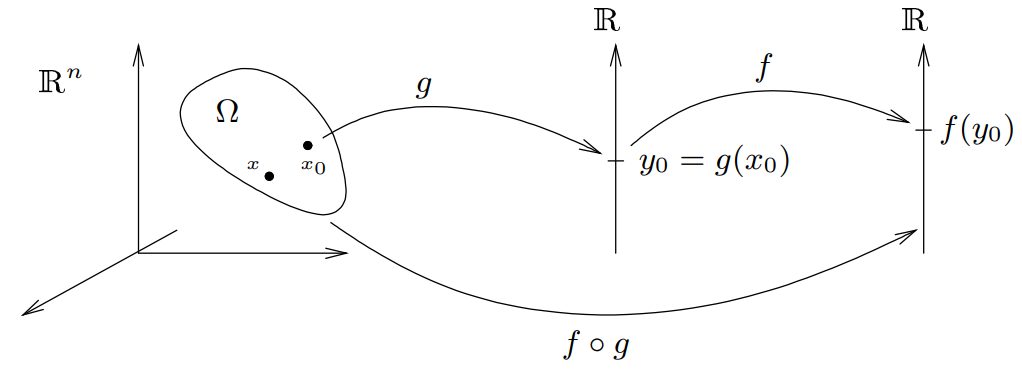
\includegraphics[width = 1\linewidth]{Bilder/Kettenregel_0.png}
            \end{center}
        \end{minipage}
        \begin{annotation}{Anmerkung}
            \item [i)] Als erstes kann df ausgerechnet werden, dann wird $g(x_0)$ fuer die einzelnen Komponenten eingesetzt. Danach werden die beiden Matrizen mutlipliziert.
            \item [ii)] Die Reihenfolge ist im Vergleich zur Kettenregl in 1D sehr wohl wichtig!
        \end{annotation}
    \end{center}


    \subsubsection{Satz: Kettenregel 2. Version}

    Sei $g: ]a,b[ \to \Omega$ an der Stelle $t_0 \in ]a,b[$ differenzierbar und sei $f: \Omega \to \R$ $\Omega \subset \R^n$ an der Stelle $g(t_0)$ differenzierbar. Dann gilt

    \begin{center}
        \begin{minipage}{0.5\linewidth}
            \begin{center}
                \eqbox{$(f \circ g)' (t_0) = \underbrace{df_{(g(t_0))}}_{\text{co-Vektor}} \cdot \underbrace{g'(t_0)}_{\text{Vektor}}$}
            \end{center}
        \end{minipage}
        \begin{minipage}{0.49\linewidth}
            \begin{center}
                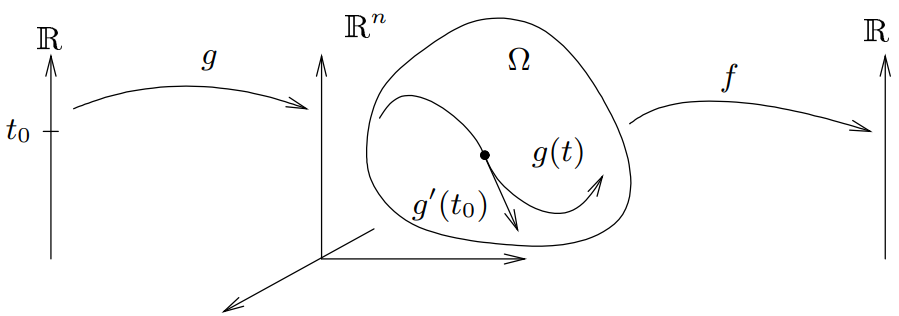
\includegraphics[width = 1\linewidth]{Bilder/Kettenregel.png}
            \end{center}
        \end{minipage}
    \end{center}


    \subsection{Richtungsableitungen}

    Sei $\Omega \subseteq \R^n$ offen und $f: \Omega \to \R$. Dann ist die Richtungsableitung eines Vektors $\vect{v} \in \R^n$ an einem Punkt $x_0$:

    \begin{center}
        \eqbox{$\partial_{\vect{v}} f(x_0) = \lim\limits_{s \to 0} \dfrac{f(x_0 + s \cdot \vect v) - f(x_0)}{s}$}
    \end{center}
    Die Richtungsableitung kann auch mithilfe des Gradienten berechnet werden. Es gilt:
    \begin{itemize}
        \item $\partial_ef(x_0)=\vec{e}\cdot\nabla f(x_0)$ \hspace{10pt} wobei $\vec{e}$ normiert ist (Länge 1)
    \end{itemize}
    \begin{annotation}{Anmerkung}
        \item [i)] Gib es im Punkt $x_0$ eine Richtungsableitung, die nicht existiert, so ist $f$ in $x_0$ nicht differenzierbar.
        \item [ii)] Es kann sein, dass alle Richtungsableitungen existieren, aber $f$ ist trotzdem nicht differenzierbar.
    \end{annotation}

    \subsubsection{Satz}

    $f$ ist differenzierbar in $x_0 \in \Omega \, \Rightarrow \partial_v f(x_0) = df_{(x_0)} \cdot \vect{v}$


    \subsection{Vektorfelder}

    Funktionen der Form $v: \Omega \subset \R^n \to \R^n$ heissen Vektorfelder. Jeder Stelle im Definitionsbereich wird ein Vektor zugeordnet.


    \subsubsection{Gradientenfeld}

    Sei $f \in C^1(\R^n)$ mit der dazugehörigen 1-Form $\lambda = df$. Das zur 1-Form zugehörige Vektorfeld heisst Gradientenfeld und ist

    \begin{center}
        \eqbox{$\displaystyle \nabla f(\vect{x}) = \sum\limits_{i = 1}^n \dfrac{\partial f}{\partial x^i}(\vect{x}) \cdot \vect{e}^i = \begin{pmatrix}
                    \frac{\partial f}{\partial x^1} \\ \vdots \\ \frac{\partial f}{\partial x^n}
                \end{pmatrix}$}
    \end{center}

    \begin{center}
        \begin{tabular}{r p{0.8\linewidth}} \toprule
            i)  & \hspace*{-10pt} $\nabla f(\vect{x}_0)$ gibt die Richtung des ''steilsten Anstiegs'' an. \\
            ii) & \hspace*{-10pt} $\nabla f(\vect{x}_0)$ ist orthogonal zu den ''Levelmengen''.           \\
            \bottomrule
        \end{tabular}
    \end{center}


    \subsection{Höhere Ableitungen}

    Sei $\Omega \subset \R^n$ offen und $f \in C^1(\Omega)$. Dann ist $f \in C^2(\Omega)$, falls

    \begin{center}
        \eqbox{$\dfrac{\partial f}{\partial x^{i}} \in C^1(\Omega), \quad \forall 1 \leq i \leq n$}
    \end{center}

    D.h. falls \textbf{alle} zweiten part. Ableitungen existieren und stetig auf $\Omega$ sind.

    \subsubsection{Satz von Hermann Schwarz}

    Sei $\Omega \subset \R^n$ offen und $f \in C^2(\Omega)$. Dann gilt

    \begin{center}
        \eqbox{$\dfrac{\partial}{\partial x^{i}}\left(\dfrac{\partial f}{\partial x^{j}}\right) = \dfrac{\partial}{\partial x^{j}} \left(\dfrac{\partial f}{\partial x^{i}} \right), \quad \forall \, 1 \leq i, j \leq n$}
    \end{center}


    \subsection{Funktionen der Klasse $C^m$}

    Sei $\Omega \subset \R^n$. $f \in C^1(\Omega)$ heisst von der Klasse $C^m$, $f \in C^m(\Omega)$, falls

    \begin{center}
        \eqbox{$\dfrac{\partial f}{\partial x^{i}} \in C^{m - 1}(\Omega), \quad \forall 1 \leq i \leq n$}
    \end{center}

    \subsubsection{Notation (Multi-Index Schreibweise)}

    Sei $\alpha = (\alpha_1, \dots, \alpha_n) \in \N^n_0$ mit $|\alpha| = \alpha_1 + \dots + \alpha_n$ und $\alpha! = \alpha_1! \cdot \dots \cdot \alpha_n!$. Dann gelten für $x = (x_1, \dots, x_n)$ folgende Notationen:

    \begin{center}
        \renewcommand{\arraystretch}{1.5}
        \begin{tabular}{r l} \toprule
            i)   & \hspace*{-10pt} $x^\alpha = x_1^{\alpha} \cdot \, \dots \, \cdot x_n^{\alpha_n}$                                                         \\
            ii)  & \hspace*{-10pt} $\partial^{\alpha} f(x) = \dfrac{\partial^{|\alpha|} f(x)}{(\partial x_{1})^{\alpha_1} \dots (\partial x_n)^{\alpha_n}}$ \\
            iii) & \hspace*{-10pt} $p(x) = \sum\limits_{|\alpha| \leq N} a_{\alpha} x^{\alpha}$                                                             \\
            \bottomrule
        \end{tabular}
    \end{center}


    \subsection{Der Satz von Taylor}

    Sei $f \in C^m(\Omega \subset \R^n)$. Für jedes $x, y \in \R^n$ existiert ein $c \in [x, y]$, so dass

    \begin{center}
        \eqboxf{$f(y) = \underbrace{\sum\limits_{|\alpha| \leq (m - 1)} \dfrac{1}{\alpha!} \partial^{\alpha}f(x) (y - x)^{\alpha}}_{=: T_{m - 1}f(y, x)} + \underbrace{\sum\limits_{|\alpha| = m} \dfrac{1}{\alpha!} \partial^{\alpha}f(c) (y - x)^{\alpha}}_{\text{Restterm}}$}
    \end{center}

    $T_k f(y,x)$ heisst das Taylor-Polynom $k-ter$ Ordnung von $f(y)$ mit dem Entwicklungspunkt $x$. \\
    Allgemein gilt:\\
    \eqbox{$T_nf(x, a)=\sum_{k=0}^{n} \frac{1}{k!}\left(\Delta x_1 \frac{\partial}{\partial x_1}+\cdots+\Delta x_n \frac{\partial}{\partial x_n}\right)^kf(x)\Bigg|_{x=a}$}
    \subsubsection{Taylorentwicklung für $n = 2$ und $m = 2$ }

    \begin{center}
        \renewcommand{\arraystretch}{2}
        \begin{tabular}{r l}
            \hspace*{-8pt} $f(y) = $ & \hspace*{-13pt} $f(x) + \frac{\partial f}{\partial x}(x) \cdot (y_1 - x_1) + \frac{\partial f}{\partial y}(x) \cdot (y_2 - x_2)$                  \\
                                     & \hspace*{-13pt} $+ \frac{1}{2!} \, [ \frac{\partial^2 f}{\partial x_1^2}(c) (y_1 - x_1)^2 + \frac{\partial^2 f}{\partial x_2^2}(c) (y_2 - x_2)^2$ \\
                                     & $ +2 \frac{\partial^2 f}{\partial x_2 \partial x_1}(c) (y_2 - x_2)(y_1 - x_1) ]$                                                                  \\
        \end{tabular}
    \end{center}

    \subsubsection{Korollar}

    Die Taylorentwicklung gibt die beste Approximation um $x$:

    \begin{center}
        \eqbox{$\lim\limits_{y \to x} \dfrac{f(y) - T_m f(y,x)}{|| y - x||^m} = 0$}
    \end{center}

    \subsection{Hesse-Matrix}

    Sei $\Omega \subset \R^n$ und $f \in C^2(\Omega)$. Die Hesse-Matrix von $f$ am Punkt $x$ ist:

    \begin{center}
        \eqboxf{$Hess_f (x) := \left(\dfrac{\partial^2 f_{(x)}}{\partial x_i \partial y_i}\right)_{1 \leq i,j \leq n} = \begin{pmatrix}
                    \frac{\partial^2 f_{(x)}}{\partial x_1^2}            & \dots  & \frac{\partial^2 f_{(x)}}{\partial x_1 \partial x_n} \\
                    \vdots                                               & \ddots & \vdots                                               \\
                    \frac{\partial^2 f_{(x)}}{\partial x_n \partial x_1} & \dots  & \frac{\partial^2 f_{(x)}}{\partial x_n^2}            \\
                \end{pmatrix}$}
    \end{center}

    $Hess_f (x)$ ist symmetrisch $\Rightarrow$ $Hess_f (x)$ \emph{diagonalisierbar} mit $\lambda_i \in \R$.

    \subsubsection{Einschub: Definitheit einer Matrix}

    \begin{tabular}{r l}
        i)  & \hspace*{-13pt} Eine Matrix ist \textbf{positiv definit}, falls alle Eigenwerte $\lambda_i > 0$. \\
        ii) & \hspace*{-13pt} Eine Matrix ist \textbf{negativ definit}, falls alle Eigenwerte $\lambda_i < 0$. \\
        ii) & \hspace*{-13pt} Eine Matrix ist \textbf{indefinit}, falls positive und negative Eigenwerte.      \\
    \end{tabular}

    \subsubsection{Kritischer Punkt}

    Ein Punkt $x_0 \in \Omega$ mit $df_{(x_0)} = 0$ (\emph{Koordinatenweise} $= 0$!) heisst kritischer Punkt von $f$.

    \subsubsection{Satz}

    Sei $f \in C^2(\Omega \subset \R^n)$. Ein kritischer Punkt $x_0$ ist eine

    \begin{center}
        \begin{tabular}{r l} \toprule
            i)   & \hspace*{-10pt} strikte lokale Minimastelle, falls $Hess_f (x_0)$ positiv definit ist. \\
            ii)  & \hspace*{-10pt} strikte lokale Maximastelle, falls $Hess_f (x_0)$ negativ definit ist. \\
            iii) & \hspace*{-10pt} ein Sattelpunkt, falls $Hess_f (x_0)$ indefinit ist.                   \\
            \bottomrule
        \end{tabular}
    \end{center}

    Bem: Bei degenerierten Punkten ($\det(Hess_f (x_0)) = 0$) kann man mit diesem Ansatz keine Aussage über lokales Min/Max/Sattelpunkt treffen!


    \subsubsection{Differentiationsregeln}

    Sei $\Omega \subset \R^n$ offen. Seien $f,g: \Omega \to \R^l$ in $x_0 \in \Omega$ differenzierbar. Es gilt

    \begin{center}
        \begin{tabular}{r l} \toprule
            i)  & \hspace*{-10pt} $d(f + g)_{x_0} = df_{(x_0)} + dg_{(x_0)}$                                                                                                \\
            ii) & \hspace*{-10pt} $d \langle f, g \rangle_{(x_0)} = \sum\limits_{i = 1}^l \left( f^{i}(x_0) \cdot dg^{i}_{(x_0)} + g^{i}(x_0) \cdot df^{i}_{(x_0)} \right)$ \\
            \bottomrule
        \end{tabular}
    \end{center}

    \subsubsection{Kettenregel 3te Version}

    Seien $g: \R^n \to \R^l$ an $x_0 \in \R^n$ und $f: \R^l \to \R^m$ an $g(x_0)$ differenzierbar.

    \begin{center}
        \eqbox{$d(f \circ g)_{(x_0)} = \underbrace{df_{(g(x_0))}}_{\in M_{m \times l}(\R)} \cdot \underbrace{dg_{(x_0)}}_{\in M_{l \times n}(\R)}$}
    \end{center}

    Es empfiehlt sich stark für $g$ und $f$ andere Koordinaten zu benutzen!


    \subsection{Der Umkehrsatz}

    Sei $\Omega \subset \R^n$ offen und $f \in C^1(\Omega, \R^n)$. Sei $df_{(x_0)} \in M_{n \times n}(\R)$ invertierbar ($\det(df_{(x_0)}) \neq 0$) an einer Stelle $x_0 \in \Omega$. Dann existieren Umgebungen

    \begin{center}
        $\exists r > 0$ so dass $f:\underbrace{B_r(x_0)}_{:= U} \to \underbrace{f(B_r(x_0))}_{:=V}$
    \end{center}

    invertierbar ist und es existiert ein $g: V \to U$ so dass

    \begin{center}
        $g(f(x)) = x, \, \forall x \in U, \quad f(g(y)) = y, \, \forall y \in V$
    \end{center}


    und $g \in C^1(V, U)$ wobei $dg_{(f(x))} = (df_{(x)})^{-1}$. ($^{-1}$ $\hat{=}$ Matrixinverse!)


    \subsubsection{Diffeomorphismus}

    Sei $U,V \subset \R^n$ offen und $\Phi \in C^1(U;V)$. Die Abbildung $\Phi$ heisst ein \emph{Diffeomorphismus} von $U$ auf $\Phi(U) = V$, falls $\Phi$ \emph{injektiv ist} und falls die Umkehrabbildung $\Phi^{-1}$ von der Klasse $C^1(V;U)$ ist. \medskip

    Aus dem Umkehrsatz folgt: Eine differenzierbare Abbildung mit invertierbarem Differential ist \emph{lokal} ein Diffeomorphismus.


    \subsubsection{Anwendung: Polarkoordinanten}

    Die Abbildung $f: (0, \infty) \times (-\pi,\pi)  \to \R^2$ mit

    \begin{center}
        $f(r, \varphi) = \begin{pmatrix}
                r \cos(\varphi) \\ r \sin(\varphi)
            \end{pmatrix}$ \qquad $df_{(r, \varphi)} = \begin{pmatrix}
                \cos(\varphi) & - r \sin(\varphi) \\ \sin(\varphi) & r \cos(\varphi) \\
            \end{pmatrix}$
    \end{center}

    erfüllt die Bedingungen vom Umkehrsatz, da

    \begin{center}
        $\det(df_{(r, \varphi)}) = r(\cos^2(\varphi) + \sin^2(\varphi)) = r > 0$
    \end{center}

    Man kann also \emph{lokal} folgende Umkehrabbildung einführen:

    \begin{center}
        $g:\begin{pmatrix}
                x \\ y \\
            \end{pmatrix} \mapsto \begin{pmatrix}
                r = \sqrt{x^2 + y^2} \\ \varphi = \arctan(y/x) \\
            \end{pmatrix}$
    \end{center}


    \subsection{Implizite Funktionen}

    Das Ziel ist es die Levelmengen / Höhenlinien ($f^{-1}(\{c\})$) zu beschreiben.

    \subsubsection{Satz}

    Sei $\Omega \subset (\R^{n-1} \times \R)$ offen und $f \in C^1(\Omega, \R)$. Man hat also \emph{eine Variable der Funktion isoliert}: $f(\underbrace{x}_{\in \R^{n - 1}}, \underbrace{y}_{\in \R})$. \medskip

    Sei ein Punkt $(x_0, y_0) \in \Omega$ mit $f(x_0, y_0) = 0$ und $\partial_y f_{(x_0,y_0)} \neq 0$. Dann existiert lokal eine Umgebung von $(x_0, y_0)$ und eine Funktion $h$:

    \begin{center}
        $h: B_r^{n - 1}(x_0) \to \R$
    \end{center}

    sodass, die Höhenlinie $f(x_0,y_0) = 0$ durch $h$ beschrieben wird:

    \begin{center}
        \eqbox{$\{(x,y) \in U; \, f(x,y) = 0\} \quad = \quad \{(x,h(x)); \, x \in B_r^{n-1}(x_0)\}$}
    \end{center}

    Insbesondere gilt $h(x_0) = y_0$ und $f(x_0,h(x_0)) = f(x_0, y_0)$. Ausserdem ist $h \in C^1(B_r^{n - 1}(x_0), \R)$ und das Differential ist:

    \begin{center}
        \eqbox{$\displaystyle dh_{(x_0)} = - \dfrac{1}{\partial_y f_{(x_0, h(x_0))}} \underbrace{\sum\limits_{i = 1}^{n - 1} \partial_{x_i} f_{(x_0, h(x_0))} \, dx_i}_{=d_x f}$}
    \end{center}

    wobei $d_x f$ das Differential von $f$ ist ohne den Koordinaten $y$.




    \subsection{Extrema mit Nebenbedingungen}

    \subsubsection{Satz: Lagrange-Multiplikatorenregel}
    Das Ziel ist es die Extrema einer Funktion $f$ zu bestimmen, welche durch eine Nebenbedingung $g$ eingeschränkt ist. \\
    Sei $U \subseteq \R^n$ offen und $M=\{x \in U | g(x)=0\}$ fuer g; $U \rightarrow \mathbb{R}^{n-k}$ (mit 0 ein regulärer Wert). \\
    Die \textbf{Lagrange-Funktion} ist definiert als:
    \begin{center}
        \eqbox{$L: (x, \lambda) \in U \times \mathbb{R}^k \rightarrow L(x, \lambda) = f(x) - \sum_{i=1}^{n-k} \lambda_i g_i(x)$}
    \end{center}
    Die Extrema von $f$ unter der Nebenbedingung $g$ sind die kritischen Punkte von $L$:
    \begin{center}
        \eqboxf{$DL(p_0)=DF(p_0)-\lambda*Dg(p_0) = 0$}
    \end{center}
    \subsubsection{Nebenbedingungen: Einfache Randmengen}

    Der Rand vom Einheitskreis ist: $\partial B_1(0) := \{(x,y) \in \R^2; x^2 + y^2 = 1\}$.

    \subsection{Vorgehen: Globale Extremewerte bestimmen}

    \begin{enumerate}
        \item Argumentieren, wieso die Menge Kompakt ist.
              \begin{itemize}
                  \item Abgeschlossenheit: Menge duch \emph{stetige} Funktionen abgegrenzt, es folgt die Menge enthält alle Randpunkte.
                  \item Beschränktheit: Auf die Ungleichung verweisen.
                  \item Kompakt: Folgern das die Menge Kompakt ist und Extremumsatz gilt.
              \end{itemize}
        \item Kritische Punkte im Inneren bestimmen (Kandidaten für Extrema).
        \item Alle Kandidaten für Extrema \emph{auf dem Rand der Menge} bestimmen. Man kann hier entweder Lagrange verwenden oder das alternative Vorgehen (siehe unten).
        \item Die Randpunkte, welche nicht erfasst werden könnnen bestimmen, \textbf{auch Kandidaten}!
        \item Alle Kandidaten in $f$ einsetzen und Minimum/Maximum bestimmen.
    \end{enumerate}

    \subsubsection{Alternatives Vorgehen für das Bestimmen der Kandidaten auf dem Rand}

    Diese Vorgehen bietet sich gut an, wenn der Rand nicht durch eine einzige Nebenbedingungen darstellbar ist. Vorgehen:

    \begin{enumerate}
        \item Man parametrisiert den Rand mithilfe von Wegen $\gamma_i(t), \, t \in [a,b]$.
        \item Man betrachtet für jeden Weg $\gamma_i$ die Funktion $f(\gamma_i)$ und analysiert, ob $f(\gamma_i)$ einen kritischen Punkt aufweist ($f'(\gamma_i) = 0$).
        \item Man \textbf{überprüft}, ob der kritische Punkt überhaupt in $t$ drinnen ist.
        \item Man nimmt zusätzlich \textbf{alle Randpunkte der Wege} als Kandidaten auf, d.h. $a, b$ eingesetzt in ihr $\gamma_i$ sind auch Kandidaten!
    \end{enumerate}



    \section{Wegintegrale}

    \subsection{Differentialform (1-Form)}

    Sei $\Omega \subset \R^n$ offen. Eine Abbildung $\lambda: \Omega \to L(\R^n,\R)$, welche jedem $x \in \Omega$ eine lineare Abbildung $\lambda(x): \R^n \to \R$ zuordnet, heisst Differentialform vom Grad 1. Es gilt ausserdem folgende Äquivalenz:

    \begin{center}
        \eqbox{1-Form: $\displaystyle \lambda(x) = \sum\limits_{i = 1}^n \lambda_i(x) d x^i$} $\Leftrightarrow$ Vektorfeld: $V(x) = \begin{pmatrix}
                \lambda_1(x) \\ \vdots \\ \lambda_n(x)
            \end{pmatrix}$
    \end{center}

    wobei $dx^{i} = (0, \dots, 0, 1, 0, \dots 0)$ die Basiselemente von $L(\R^n, \R)$ sind. \medskip

    Bemerkung: Für jedes $f \in C^1(\Omega)$ ist das Differential $df$ eine 1-Form.


    \subsection{Wegintegral}

    Ein Weg ist eine vektorwertige Funktion $\gamma \in C^1_{stw}([a,b], \R^n)$. Man sagt:

    \begin{center}
        \begin{tabular}{r p{0.8\linewidth}} \toprule
            i)  & \hspace*{-10pt} $\gamma(a)$ und $\gamma(b)$ sind seine Anfangs- und Endpunkte.         \\
            ii) & \hspace*{-10pt} Die Ableitung $\dot \gamma$ ist der Geschwindigkeitsvektor.            \\
            ii) & \hspace*{-10pt} Wenn $\gamma(a) = \gamma(b)$ gilt, dann heisst $\gamma$ abgeschlossen. \\
            \bottomrule
        \end{tabular}
    \end{center}

    Sei $\gamma_1, \gamma_2 \in C^1_{stw}([0,1], \R^n)$ mit $\gamma_1(1) = \gamma_2(0)$. Dann ist $\gamma = \gamma_1 + \gamma_2$:

    \begin{center}
        $\gamma: [0,2] \to \Omega$ mit $t \mapsto \begin{cases}
                \gamma_1(t)     & t \in [0,1] \\
                \gamma_2(t - 1) & t \in [1,2] \\
            \end{cases}$
    \end{center}

    Es gilt ausserdem: $\displaystyle \int_{\gamma_1 + \gamma_2} \lambda = \int_{\gamma_1} \lambda + \int_{\gamma_2} \lambda$

    \subsubsection{Das Wegintegral}

    Sei $\gamma \in C^1_{stw}([a,b], \R^n)$ und $\lambda$ eine 1-Form mit dem zu $\lambda$ zugehörigem Vektorfeld $V$. Dann ist das Wegintegral:

    \begin{center}
        \eqboxf{$\displaystyle \int_\gamma \lambda := \int\limits_a^b \lambda(\gamma(t)) \cdot \dot \gamma(t) dt \, \Leftrightarrow \,  \int_\gamma V \, d\vec{s} = \int\limits_a^b \langle V_i(\gamma(t)), \dot\gamma \rangle dt$}
    \end{center}

    Das Wegintegral ist \emph{unabhängig} von orientierungserhaltenden Umparametrisierungen von $\gamma$.


    \subsubsection{Einschub: Wegzusammenhängend}

    Sei $\Omega \subset \R^n$ offen. $\Omega$ heisst \emph{wegzusammenhängend}, falls jedes Paar von Punkten in $\Omega$ mit einem Weg verbunden werden kann.


    \subsubsection{Satz}

    Sei $\Omega$ offen und Wegzusammenhängend.

    \begin{center}
        \eqbox{$f \in C^1(\Omega)$ mit $df = 0 \, \Leftrightarrow f$ ist konstant}
    \end{center}

    \subsubsection{Einschub: Parametrisierungen}

    \begin{tabular}{r l l}
        Gerade von $a$ nach $b$:        & \hspace*{-12pt} $\gamma(t) = (1-t) \cdot a + t \cdot b$                       & \hspace*{-5pt} $t \in [0,1]$     \\
        Kreis (positiven Sinne):        & \hspace*{-12pt} $\gamma(t) = (r\cdot \cos(\varphi), r \cdot \sin(\varphi))$   & \hspace*{-5pt} $t \in [0, 2\pi]$ \\
        Kreis (\emph{negativen} Sinne): & \hspace*{-12pt} $\gamma(t) = (r\cdot \cos(\varphi), - r \cdot \sin(\varphi))$ & \hspace*{-5pt} $t \in [0, 2\pi]$ \\
        Ellipse (positive Sinne):       & \hspace*{-12pt} $\gamma(t) = (a \cdot \cos(t), b \cdot \sin(t))$              & \hspace*{-5pt} $t \in [0,2\pi]$  \\
    \end{tabular}




    \subsection{Potentiale}

    Sei $\Omega \subset \R^d$ offen und $\lambda \in C^0(\Omega, \R^n)$ eine 1-Form. Es sind \textbf{äquivalent}: \medskip

    i) $\exists f \in C^1(\Omega)$ mit \eqbox{$\lambda = df$} \quad ($f$ heisst ''Potential von $\lambda$'') \medskip

    ii) Für je zwei Wege $\gamma_1, \gamma_2 \in C^1_{stw}([a,b], \Omega)$ mit $\gamma_1(a) = \gamma_2(a), \, \gamma_1(b) = \gamma_2(b)$, d.h. mit \emph{gleichen Anfangs- und Endpunkten}, gilt:

    \begin{center}
        \eqboxf{$\displaystyle \int\limits_{\gamma_1} \lambda = \int\limits_{\gamma_2} \lambda = f(\gamma(b)) - f(\gamma(a))$}
    \end{center}

    iii) Für jeden \textbf{geschlossenen} Weg $\gamma \in C^1_{stw}([a,b], \Omega)$ mit $\gamma(a) = \gamma(b)$:

    \begin{center}
        \eqbox{$\displaystyle \int\limits_{\gamma} \lambda = 0$} \quad (''$V$ ist \emph{konservativ}'')
    \end{center}

    Bem: Potentiale sind bis auf die Addition einer Konstante bestimmt!


    \subsubsection{Verfahren zur Berechnung eines Potentials}

    Sei $\lambda$ eine 1-Form. Das zugehörige Potential $f$, falls es existiert, kann man mit folgendem Verfahren ermitteln: \medskip

    i) Wir setzen oBdA:  $f(0,0,0) = 0$ \medskip

    ii) Wir nehmen die folgenden drei Wegintegrale:

    \begin{center}
        $\gamma_1(t) = \begin{pmatrix}
                t \, x \\ 0 \\ 0 \\
            \end{pmatrix}, \, \gamma_2(t) = \begin{pmatrix}
                x \\ t \, y \\ 0 \\
            \end{pmatrix}, \, \gamma_3(t) = \begin{pmatrix}
                x \\ y \\ t \, z \\
            \end{pmatrix}$
    \end{center}

    iii) Aus dem zweiten Punkt im vorherigen Satz folgt:

    \begin{center}
        $\displaystyle f(x,y,z) = f(0,0,0) + \int_{\gamma_1 + \gamma_2 + \gamma_3} \lambda = \int_{\gamma_1} \lambda + \int_{\gamma_2} \lambda + \int_{\gamma_3} \lambda$
    \end{center}

    \begin{center}
        \begin{minipage}{0.35\linewidth}
            \begin{center}
                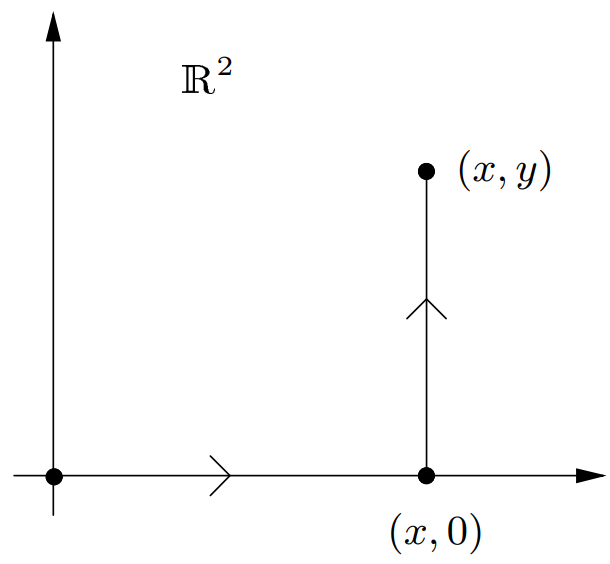
\includegraphics[width=1\linewidth]{Bilder/Potential.png}
            \end{center}
        \end{minipage}
        \begin{minipage}{0.64\linewidth}
            iv) Zum Schluss: \textbf{Verifizieren}, dass $f$ wirklich das Potential von $\lambda$ ist:

            \begin{center}
                \eqbox{$df(x,y,z) = \lambda$}
            \end{center}
        \end{minipage}
    \end{center}

    \subsubsection{Satz: Potentialfeld}

    Für ein Vektorfeld $V \in C^0(\Omega, \R^n)$ sind äquivalent:

    \begin{center}
        \eqbox{$V$ ist konservativ $\Leftrightarrow$ $\exists f \in C^1(\Omega): V = \nabla f$}
    \end{center}

    In diesem Fall heisst $V$ \textbf{Potentialfeld} mit dem Potential $f$.


    \subsubsection{Korollar: Rotationsvektorfeld}

    Sei $V = (V_1, \dots, V_n) \in C^1(\Omega, \R^n)$ konservativ. Dann gilt

    \begin{center}
        \eqbox{$\dfrac{\partial V^{i}}{\partial x^{j}} - \dfrac{\partial V^{j}}{\partial x^{i}} = 0, \quad \forall \, 1 \leq i,j \leq n$}
    \end{center}

    \section*{Untermannigfaltigkeiten}
    \subsection*{Definition}

    Sei $M \subseteq \mathbb{R}^n$ und $p \in M$. Wir sagen, dass
    M um p eine d-dimensionale $C^k$-Untermannigfaltigkeit des $\mathbb{R}^n$ ist genau dann wenn es
    eine offene Umgebung $U_p \subseteq \mathbb{R}^n$ von p, eine Permutation $\sigma$ von $\{1, . . . , n\}$, eine offene
    Teilmenge $V_p \subseteq \mathbb{R}^d$ und eine Funktion $f \in C^k (V, R^{n-d} )$ gibt, sodass
    \begin{center}
        \eqbox{$\{(x_{\sigma(1)}, \dots, x_{\sigma(n)}):x \in M \cap U_p\} = graph(f) = \{(y,f(y)): y \in V_p\}$}
    \end{center}
    Falls dies fuer alle Punkte $p \in M$ gilt, so nennen wir M eine d-dimensionale $C^k$-Untermannigfaltigkeit des $\mathbb{R}^n$
    Die Funktion kann also lokal als Graph einer Funktion dargestellt werden, welche eine kleinere Dimension haben kann.
    \subsection*{Immersion, Submession}
    $\textbf{Immersion}$: $f$ ist in $p$ eine Immersion genau dann wenn $df(p)$ injektiv ist. Falls $f$ für
    alle $p \in U$ eine Immersion ist, dann ist $f$ eine Immersion.
    Eine Matrix ist genau dann injektiv, wenn gilt:
    \begin{center}
        \eqbox{$Rang(M) = $ Anzahl der Spalten der Matrix}
    \end{center}
    $\textbf{Submersion}$: $f$ ist in $p$ eine Submersion genau dann wenn $df(p)$ surjektiv ist. Falls $f$ für
    alle $p \in U$ eine Submersion ist, dann ist $f$ eine Submersion.
    Eine Matrix ist genau dann surjektiv, wenn gilt:
    \begin{center}
        \eqbox{$Rang(M) = $ Anzahl der Zeilen der Matrix}
    \end{center}
    \subsection*{Einbettung}
    Sei $V \subseteq \mathbb{R}^d$ offen und $\psi: V \rightarrow \mathbb{R}^n$.
    Wie nenen $\psi$ eine $C^k$ Einbettung, wenn:
    \begin{itemize}
        \item $\psi$ eine Immersion ist
        \item $\psi$  $C^k$ ist
        \item $\psi$ injektiv ist
        \item $\psi^{-1}$ stetig ist
    \end{itemize}
    Falls $\psi$ eine $C^k$ Einbettung ist, dann ist das Bild $\psi(V)$ eine $C^k$-Untermannigfaltigkeit des $\mathbb{R}^n$ der Dimension d.
    (Eine Einbettung stellt also eine Funktion dar, die von der tieferen d-Dimension in die hoere n-Dimension geht und die Untermannigfaltigkeit einbettet in den umliegenden Raum).
    \subsection*{Satz vom regulären Wert}
    \subsubsection*{Regulärer Wert}
    Sei $U_0 \in \mathbb{R}^n$ offen, $g \in C^k (U_0 ; R^l )$ und $z_0 \in \mathbb{R}^l$ . Dann
    ist $y_0$ ein regulärer Wert für g genau dann wenn g eine $\textbf{Submersion}$ ist in jedem Punkt
    von
    \begin{center}
        \eqbox{$g^{-1}(z_0) = \{x \in U_0 : g(x) = z_0\}$}
    \end{center}
    Sonst ist $z_0$ ein singulärer Wert von g.
    \subsubsection*{Satz vom regulären Wert}
    Das Urbild jedes regulären Wertes ($g^{-1}(z_0)$) ist eine $C^k$-Untermannigfaltigkeit des $\mathbb{R}^n$ mit der Dimension $n-l$.\\
    \begin{example}
        \textbf{Beispiel}\\
        Die Funktion $g: \mathbb{R}^2 \rightarrow \mathbb{R}$ mit $g(x,y) = x^2 + y^2$ hat den regulären Wert $1$. Das Urbild von $1$ ist der Einheitskreis, welcher eine 1-dimensionale Untermannigfaltigkeit des $\mathbb{R}^2$ ist.
    \end{example}
    \subsection*{Tangentialraum}
    Sei $M \subseteq \mathbb{R}^n$ eine d-dimensionale Teilmannigfaltigkeit Der Tangentialraum von M bei $p \ in M$ ist definiert durch:
    \begin{center}
        \eqboxbig{$T_pM=\{(p,\gamma'(0)):\exists \epsilon > 0, \gamma: (-\epsilon, \epsilon) \rightarrow M$ differenzierbar mit $\gamma(0) = 0\}$ $\subseteq T_p \mathbb{R}^n = \{p\} \times \mathbb{R}^n$}
    \end{center}
    Der Tangentialraum ist die Menge aller Geschwindigkeitsvektoren von kurzen Wegen durch p in M.
    Der Tangentialraum von $c^1$-Untermannigfaltigkeiten der Dimension d im Punkt $x_0 \in M$ (wobei $M \subseteq \mathbb{R}^n$) kann folgendermassen berechnet werden:
    \begin{center}
        \begin{itemize}
            \item Sei $U \subseteq \mathbb{R}^n$ eine offene Umgebung von $x_0, V \subseteq \mathbb{R}^d$
                  offen und $f \in C^1(V, \mathbb{R}^{n-d})$, so dass:
                  \begin{center}
                      $M \cap =$ graph(f) = $\{(y, f(y)):y \in V\}$
                  \end{center}
                  Wir bezeichnen die erste Komponente von $x_0 \in \mathbb{R}^d \times \mathbb{R}^{n-d}$ mit $y_0$. Der Tangentialraum kann berechnet werden als:
                  \begin{center}
                      \eqbox{$T_{x_0}M = graph(Df(y_0))$}
                  \end{center}
            \item Sei $y_0 \in V$ und $\psi : V \rightarrow \mathbb{R}^n$ so, dass:
                  \begin{center}
                      $\psi(y_0)=x_0. \vspace*{10pt} \psi(V)=M \cap U$
                  \end{center}
                  und $\psi$ im Punkt $y_0$ eine Immersion. Dann der Tangentialraum berechnet werden aus:
                  \begin{center}
                      \eqbox{$T_{x_0}M = im(D\psi(y_0))$}
                  \end{center}
            \item Sei $g:U \rightarrow \mathbb{R}^{n-d}$ so, dass
                  \begin{center}
                      $M \cap U = g^{-1}(g(x_0))$
                  \end{center}
                  und g im Punkt $x_0$ eine Submersion ist. Dann kann der Tangentialraum berechnet werden als:
                  \begin{center}
                      \eqbox{$T_{x_0}M = ker(Dg(x_0))$}
                  \end{center}
        \end{itemize}
    \end{center}
    \vspace*{10pt}
    \begin{example}
        \textbf{Beispiel}\\
        Der Tangentialraum in jedem Punkt von $M = \{x \in \mathbb{R}^2: x_1 x_2=1\}$ ist gegeben als:\\
        1. Da 1 ein regulärer Wert von $g(x_1,x_2)=x_1 x_2$ ist, ist $M$ eine 1-dimensionale Untermannigfaltigkeit des $\mathbb{R}^2$. \\
        2. Der Tangentialraum in jedem Punkt von $M$ ist gegeben als:
        \begin{center}
            $Dg(x)= \begin{pmatrix} x_2, x_1 \end{pmatrix}$ \\
            $ker(Dg(x))=\{v \in \mathbb{R}^2:Dg(x)*v=0\} = \{(v_1, v_2) \in \mathbb{R}^2:x_2v_1+x_1v_2=0\}$ \\
            $\Rightarrow v_2=-\frac{x_2}{x_1}v_1 =-\frac{1}{x_1^2}*v_1$ \\
            $\Rightarrow ker(Dg(x)) = \{(t, -\frac{1}{x_1^2}t):t \in \mathbb{R}\} = T_xM$
        \end{center}
    \end{example}
    \section{Integration in $\R^n$}


    \subsection{Riemannsches Integral über einen Quader}

    Ein $n$-dimensionaler \emph{Quader} ist ein Produkt von Intervallen

    \begin{center}
        $\displaystyle Q = \prod\limits_{i = 1}^n I_i = \{x = (x^{i})_{1 \leq i \leq n}; x^{i} \in I_i, 1 \leq i \leq n\}$
    \end{center}

    Solch ein Quader $Q$ hat den folgenden \emph{Elementarinhalt}:

    \begin{center}
        \eqbox{$\displaystyle \mu(Q) = \mu([a,b] \times [c,d]) = \prod\limits_{i = 1}^n \left| I_i \right|$}
    \end{center}

    \begin{center}
        \begin{minipage}{0.74\linewidth}
            Die \emph{Zerlegung} $P = \{Q_k; 1 \leq k \leq K\}$ eines Quaders in disjunkte Teilquader $Q = \bigcup\limits_{k = 1}^K$ hat folgende \emph{Feinheit}:

            \begin{center}
                $\delta_P = \max\limits_{1 \leq k \leq K} diam (Q_k)$
            \end{center}
        \end{minipage}
        \begin{minipage}{0.25\linewidth}
            \begin{center}
                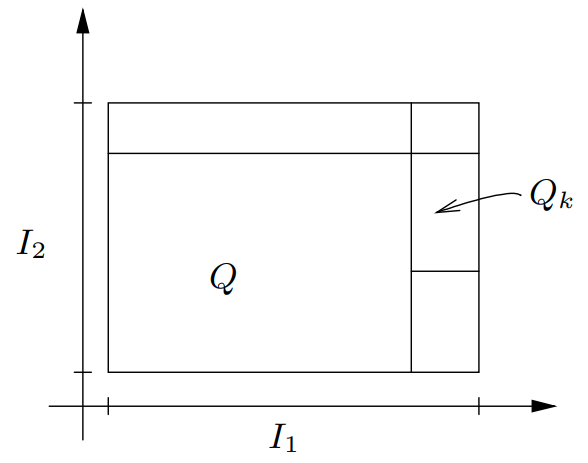
\includegraphics[width=1\linewidth]{Bilder/Quader.png}
            \end{center}
        \end{minipage}
    \end{center}

    wobei $diam (Q_k)$ den \emph{Durchmesser} von $Q_k$ bezeichnet:

    \begin{center}
        $diam(Q_k) = \sup\limits_{x,y \in Q_k} \left| x - y \right|, \, 1 \leq k \leq K$
    \end{center}

    \subsubsection{Treppenfunktion in $\R^n$}

    Eine Funktion $f: Q \to \R$ auf einem Quader $Q$ heisst Treppenfunktion, falls $f(x)$ eine Darstellung folgender Form besitzt

    \begin{center}
        \eqbox{$\displaystyle f(x) = \sum\limits_{k = 1}^K c_k \cdot \chi_{Q_k}(x)$ wobei $\chi_{Q_k}(x) = \begin{cases}
                    1 & , x \in Q_k \\ 0 & , x \not\in Q_k \\
                \end{cases}$}
    \end{center}

    mit einer Zerlegung $P = \{Q_k; 1 \leq k \leq K\}$ und Konstanten $c_k \in \R$. \medskip

    Das Riemann-Integral einer Treppenfunktion $f(x)$ ist, wie folgt definiert:

    \begin{center}
        \eqbox{$\displaystyle\int_Q f(x) \,d\mu = \sum\limits_{k = 1}^K c_k \cdot \mu(Q_k)$}
    \end{center}

    \subsubsection{Satz: Verfeinerung der Zerlegung}

    Eine Zerlegung $\tilde{P} = \{\tilde{Q}_j; \, 1 \leq j \leq J\}$ ist eine Verfeinerung der Zerlegung $P = \{Q_k; 1 \leq k \leq K\}$, falls jedes $\tilde{Q}_j$ in einem Quader $Q_k$ enthalten ist. \medskip

    Das Integral wird durch eine Verfeinerung \textbf{nicht} verändert.


    \subsection{Das Riemann Integral}

    Seien $e^-,e^+$ Treppenfunktionen und $f: Q \to \R$ beschränkt. Dann gilt:

    \begin{center}
        Untere R-Integral von $f$: \, \eqbox{$\displaystyle\underline{\int_Q} f(x) \,d\mu = \sup\limits_{e^-(x) \leq f(x)} \int_Q e^-(x) \,d\mu$} \medskip

        Obere R-Integral von $f$: \eqbox{$\displaystyle\overline{\int_Q} f(x) \,d\mu = \inf\limits_{f(x) \leq e^+(x)} \int_Q e^+(x) \,d\mu$}
    \end{center}

    Die Funktion $f$ heisst \emph{R-integrabel} über $Q$, falls

    \begin{center}
        \eqboxf{$\displaystyle\underline{\int_Q} f(x) \,d\mu = \overline{\int_Q} f(x) \,d\mu =: \int_Q f(x) \,d\mu$}
    \end{center}




    \subsubsection{Satz}

    Sei $f \in C^0(Q)$. Dann ist $f$ über $Q$ R-integrabel.

    \subsubsection{Satz: Riemannsche Summen}

    Für jede Folge von Zerlegungen $(P^{(l)})_{l \in \N}$ von $Q$ mit Feinheit $\delta_{P^{(l)}} \xrightarrow[]{l \to \infty} 0$ gilt für eine beliebige Auswahl von Punkten $x_k^{(l)} \in Q_k^{(l)}$ stets

    \begin{center}
        \eqbox{$\displaystyle \int_Q \left(\sum\limits_{k = 1}^{K^{(l)}} f(x_k^{(l)}) \chi_{Q_k^{(l)}}\right) d \mu = \sum\limits_{k = 1}^{K^{(l)}} f(x_k^{(l)}) \cdot \mu(Q_k^{(l)}) \xrightarrow[]{l \to \infty} \int_Q f \,d\mu$}
    \end{center}


    \subsection{Eigenschaften des Riemannschen Integrals}

    \subsubsection{Linearität}

    Seien $f, g: Q \to \R$ beschränkt und über $Q$ R-integrabel, und $a \in \R$.

    \begin{center}
        \eqbox{$\displaystyle \int_Q \left( \alpha \cdot f(x) + g(x) \right) \,d\mu = \alpha \cdot \int_Q f(x) \,d\mu + \int_Q  g(x) \,dx$}
    \end{center}

    \subsubsection{Monotonie}

    Seien $f,g: Q \to \R$ beschränkt und über $Q$ R-integrabel, und sei $f \leq g$.

    \begin{center}
        \eqbox{$\displaystyle \int_Q f(x) \, d\mu \leq \int_Q g(x) \, d\mu$}
    \end{center}

    Insbesondere gilt für $f \in C^0(\overline{Q})$ die Abschätzung

    \begin{center}
        \eqbox{$\displaystyle \left| \int_Q f(x) \, d\mu \right| \leq \int_Q \left| f(x) \right| \, d\mu \leq \sup\limits_{Q} \left| f(x) \right| \cdot \mu(Q)$}
    \end{center}

    \subsubsection{Korollar}

    Seien $f, f_k \in C^0(\overline{Q})$ mit $f_k \xrightarrow[]{glm.} f(k \to \infty)$. Dann gilt

    \begin{center}
        \eqbox{$\displaystyle\left| \int_Q f_k \,d\mu - \int_Q f \,d\mu \right| \leq \int_Q | f_k - f | \, d\mu \leq ||f_k - f || \cdot \mu(Q) \xrightarrow[]{(k \to \infty)} 0$}
    \end{center}

    \subsubsection{Gebietsadditivität}

    Sei $f: Q \to \R$ beschränkt und über $Q$ R-integrabel. Sei $P = \{Q_k; \, 1 \leq k \leq K\}$ eine Zerlegung von $Q$ in disjunkte Quader $Q_k$. Dann gilt

    \begin{center}
        \eqbox{$\displaystyle\int_Q f(x) \,d\mu = \sum\limits_{k = 1}^K \int_{Q_k} f(x) \,d\mu$}
    \end{center}



    \subsection{Satz von Fubini}

    Sei $Q = [a,b] \times [c,d] \subset \R^2$ \textbf{und} sei $f \in C^0(Q)$. Dann gilt

    \begin{center}
        \eqboxf{$\displaystyle\int_Q f(x,y) \,d\mu = \int\limits_a^b \left( \int\limits_c^d f(x,y) \,dy \right) dx = \int\limits_c^d \left( \int\limits_a^b f(x,y) \,dx \right) dy$}
    \end{center}

    Analoges gilt auch in höheren Dimensionen, solange $f \in C^0(Q)$ ist.




    \subsection{Jordan-Bereiche}

    Sei $\Omega \subset \R^n$ beschränkt und $Q$ ein \emph{beliebiger} Quader mit $\Omega \subset Q$.

    \begin{center}
        \begin{minipage}{0.25\linewidth}
            \begin{center}
                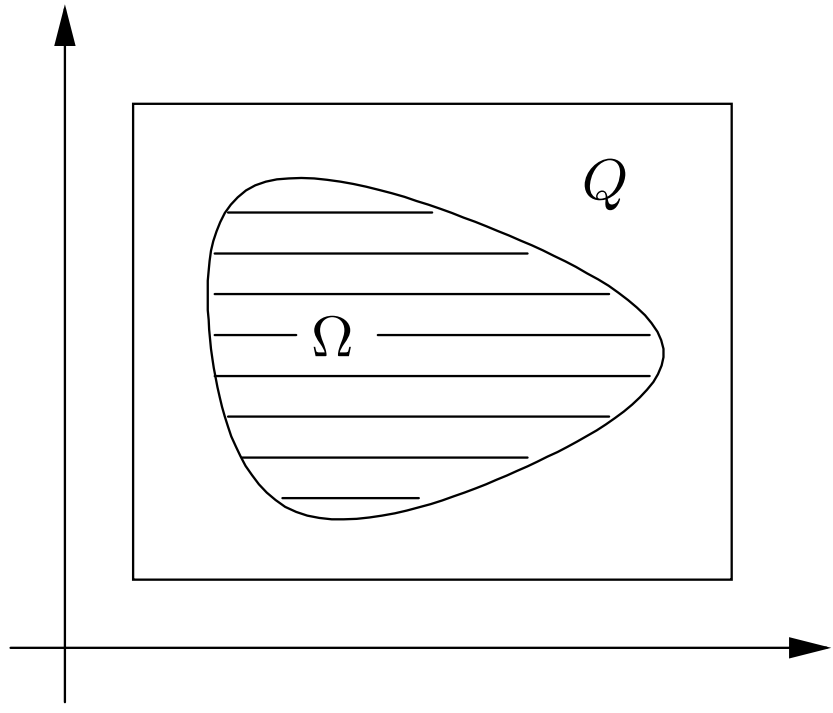
\includegraphics[width=1\linewidth]{Bilder/Jordan-Messbar.png}
            \end{center}
        \end{minipage}
        \begin{minipage}{0.74\linewidth}
            Sei $\chi_\Omega$ die charakteristische Funktion:

            \begin{center}
                $\chi_\Omega(x) = \begin{cases}
                        1 & x \in \Omega \\ 0 & x \not\in \Omega \\
                    \end{cases}$
            \end{center}
        \end{minipage}
    \end{center}

    \subsubsection{Jordan-messbar (JM)}

    Die Menge $\Omega$ heisst \emph{Jordan-messbar}, falls $\chi_\Omega(x)$ R-integrabel über $Q$ ist, diese Eigenschaft ist vom Quader $Q$ das $\Omega$ enthält \textbf{unabhängig}. \medskip

    Das n-dimensionale Jordansche Mass von $\Omega$: \eqbox{$\displaystyle \mu(\Omega) = \int_Q \chi_{\Omega}(x) \,d\mu$}

    \subsubsection{Satz}

    Seien $\Omega_1, \Omega_2$ \emph{JM}. Dann sind $\Omega_1 \cap \Omega_2$ und $\Omega_1 \cup \Omega_2$ auch \emph{JM} und

    \begin{center}
        \eqbox{$\mu(\Omega_1) + \mu(\Omega_2) = \mu(\Omega_1 \cup \Omega_2) + \mu(\Omega_1 \cap \Omega_2)$}
    \end{center}

    \subsubsection{R-Integral über Jordan-messbare Bereiche}

    Sei $\Omega \subset Q$ \emph{JM} und $f: \Omega \to \R$ beschränkt. $f$ heisst \textbf{R-Integrabel über} $\Omega$ , falls die Fortsetzung $\overline{f}$ von $f$ über $Q$ R-integrabel ist und es gilt:

    \begin{center}
        \eqbox{$\overline{f} = \begin{cases}
                    f(x) & x \in \Omega \\ 0 & x \in Q \setminus \Omega \\
                \end{cases} \qquad \displaystyle \int_\Omega f\, d\mu := \int_Q \overline{f}\, d\mu$}
    \end{center}

    \subsubsection{Satz}

    Sei $\Omega$ \emph{JM} und $f \in C^0(\Omega)$ beschränkt. Dann ist $f$ auf $\Omega$ R-Integrabel.


    \subsection{Hypograph und Hypergraph}

    Sei $Q' \subset \R^{n-1}$ und $\psi \in C^0_{stw}(\overline{Q'})$ mit $\psi \geq 0$. Dann ist die Menge

    \begin{center}
        \eqbox{$\Omega_{\psi} = \{ (x', x_n) \in \R^n ; \, x' \in Q', \, 0 \leq x_n \leq \psi(x') \}$}
    \end{center}

    Jordan-messbar und heisst \textbf{Hypograph}. \medskip

    Sei $Q' \subset \R^{n-1}$ und $\phi  \in C^0_{stw}(\overline{Q'})$ mit $\phi \leq 0$. Dann ist die Menge

    \begin{center}
        \eqbox{$\Omega_{\phi} = \{ (x', x_n) \in \R^n ; \, x' \in Q', \, \phi(x') \leq x_n \leq 0 \}$}
    \end{center}

    Jordan-messbar und heisst \textbf{Hypergraph}. \medskip

    Die Beschränkung der Menge ist flexibel, also man kann auch:

    \begin{center}
        \eqboxf{$\Omega = \{ (x, y) \in \R^2 ; \, x \in [a,b] , \,\phi(x) \leq y \leq \psi(x)\}$}
    \end{center}

    Das zugehörige Integral ist für den Fall $\R^2$:

    \begin{center}
        \eqbox{$\displaystyle \int_{\Omega} f \, d\mu = \int\limits_{a}^b \left(\, \int\limits_{\phi(x)}^{\psi(x)} f(x,y) dy \right) dx$}
    \end{center}




    \subsection{Satz von Green}

    Sei $\Omega \subset Q \subset \R^2$ ein Gebiet der Klasse $C^1_{stw}$ und $g, h \in C^1(\overline{\Omega})$. Es gilt

    \begin{center}
        \eqboxf{$\displaystyle \int_\Omega \left(\dfrac{\partial h}{\partial x} (x,y) - \dfrac{\partial g}{\partial y}(x,y) \right) \,d\mu = \int_{\partial\Omega} \underbrace{g(x,y) \,dx + h(x,y)\, dy}_{:= \lambda}$}
    \end{center}

    wobei der Rand von $\Omega$ so parametrisiert wird, dass $\Omega$ \textbf{zur Linken} liegt.
    Falls $\gamma:[a, b] \rightarrow \partial \Omega$ eine solche Parametrisierung ist, so gilt:
    \begin{center}
        $\iint_\Omega \ rot(\textbf{K}(x,y)) \ d\mu $ = $\int_{\partial \Omega} <\textbf{K}(\gamma (t)), \dot{\gamma}(t)> \ dt$
    \end{center}

    \subsubsection{Gebiet der Klasse $C^1_{stw}$ in $\R^2$}

    Sei $\Omega \subset Q$ (beschränkt). Ein Gebiet $\Omega$ ist von der Klasse $C^1_{stw}$, falls \textbf{zu jedem} Punkt $p \in \partial\Omega$ folgendes existiert:

    \begin{center}
        \begin{minipage}{0.74\linewidth}
            i) Falls notwendig, \emph{eine Drehung der Koordinatenachsen}, d.h. von $(x,y)$ zu $(x_1, x_2)$:

            \begin{center}
                $\begin{pmatrix}
                        x_1 \\ x_2 \\
                    \end{pmatrix} = \begin{pmatrix}
                        \cos(\Theta)  & \sin(\Theta) \\
                        -\sin(\Theta) & \cos(\Theta) \\
                    \end{pmatrix} \begin{pmatrix}
                        x \\ y \\
                    \end{pmatrix}$
            \end{center}

            ii) Es $\exists$ ein Quader $[a,b] \times [c,d]$ in den neuen Koordinaten $(x_1, x_2)$, welcher $p \in (a,b) \times (c,d)$ erfüllt.
        \end{minipage}
        \begin{minipage}{0.25\linewidth}
            \begin{center}
                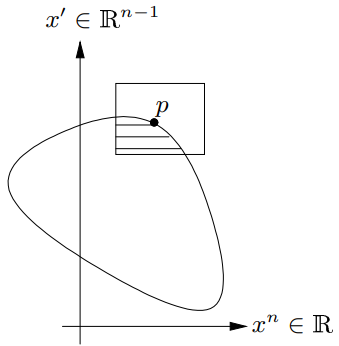
\includegraphics[width=1\linewidth]{Bilder/Stueckweise_Gebit.png}
            \end{center}
        \end{minipage}
    \end{center}

    iii) Es $\exists \psi \in C^1_{stw}([a,b],[c,d])$ und die Schnittmenge $\Omega \cap (a,b)\times(c,d)$ ist ein \emph{Hyper-/Hypograph}.

    \subsubsection{Satz von Green mit Vektorfeld}

    Sei $\Omega \subset \R^2$ beschränkt und von der Klasse $C^1_{stw}$. Sei $V = \begin{pmatrix}
            V_1(x,y) \\ V_2(x,y) \\
        \end{pmatrix}$ ein $C^1(\overline{\Omega};\R^2)$ Vektorfeld. Dann gilt:


    \begin{center}
        \begin{minipage}{0.54\linewidth}
            \begin{center}
                \eqbox{$\text{rot(V)} = \partial_x V_2 (x,y) - \partial_y V_1(x,y)$}
            \end{center}
        \end{minipage}
        \begin{minipage}{0.45\linewidth}
            \begin{center}
                \eqboxf{$\displaystyle \int_\Omega \text{rot(V)} \,d\mu = \int_{\partial\Omega} V \, d\vec{s}$}
            \end{center}
        \end{minipage}
    \end{center}

    wobei $\text{rot}(V)$ die Rotation von $V$ ist und $\partial\Omega$ ist so parametrisiert, dass $\Omega$ \textbf{zur Linken} liegt. \medskip

    Bem: Wenn $rot(V) = 1$ ist, dann kann man \emph{die Fläche} $\mu(\Omega)$ berechnen.


    \subsection{Satz von Poincaré}

    Sei $\Omega \subset \R^2$ ein beschränktes, einfach zusammenhängendes $C^1_{stw}$ Gebiet und sei $V$ ein $\R^2$-Vektorfeld der Klasse $C^1(\overline{\Omega}, \R^2)$. Dann gilt:

    \begin{center}
        \eqboxf{$V$ ist konservativ ($V = \nabla f$) $\Leftrightarrow$ rot($V) = 0$}
    \end{center}

    \subsubsection{Einschub: Einfach zusammenhängende Gebiete}

    Sei $\Omega \subset \R^2$ beschränkt, von der Klasse $C^1_{stw}$ und wegzusammenhängend. $\Omega$ heisst einfach zusammenhängend, falls $\partial\Omega$ nur eine 'Komponente' hat. \medskip

    Informell: $\Omega$ besitzt keine 'Löcher'.




    \subsection{Substitutionsregel}

    \subsubsection{Einschub: Diffeomorphismus}

    Sei $U,V \subset \R^n$ offen und $\Phi \in C^1(U;V)$. Die Abbildung $\Phi$ heisst ein Diffeomorphismus von $U$ auf $\Phi(U) = V$, falls $\Phi$ \emph{injektiv ist} und falls die Umkehrabbildung $\Phi^{-1} \in C^1(V;U)$. \medskip

    Aus dem Umkehrsatz folgt: $\Phi \in C^1(U;V)$ Diffeomorphismus $\Leftrightarrow$

    \begin{center}
        \eqbox{ $\Phi$ injektiv und $det(d\Phi_{(x_0)}) \neq 0, \forall x_0 \in U$}
    \end{center}

    \subsubsection{Transformationssatz}

    Sei $U,V \subset \R^n$ offen und $\Phi \in C^1(U,V)$ ein Diffeomorphismus. Sei $\overline{\Omega} \subset U$ beschränkt und Jordan messbar. Dann ist $\Phi(\Omega)$ Jordan messbar, und

    \begin{center}
        \eqbox{$\displaystyle \mu(\Phi(\Omega)) = \int_{\Omega} |\det(d\Phi(x))| d\mu(x)$}
    \end{center}

    wobei $\mu(\Phi(\Omega))$ das \textbf{Volumen} von $\Phi(\Omega)$ ist.

    \subsubsection{Satz: Substitutionsregel}

    Sei $U,V \subset \R^n$ offen, $\Phi \in C^1(U,\R^n)$ ein Diffeomorphismus von $U$ auf $V \subset \R^n$. Sei $\Omega \subset U$ beschränkt und Jordan messbar, und sei $f:\Phi(\Omega) \to \R$ beschränkt und R-integrabel. Dann gilt

    \begin{center}
        \begin{minipage}{0.6\linewidth}
            \begin{center}
                \eqboxf{$\displaystyle \int_{\Phi(\Omega)} f \, d\mu = \int_{\Omega} (f \circ \Phi) \cdot |\det(d\Phi)| \, d\mu$}
            \end{center}
        \end{minipage}
        \begin{minipage}{0.39\linewidth}
            \begin{center}
                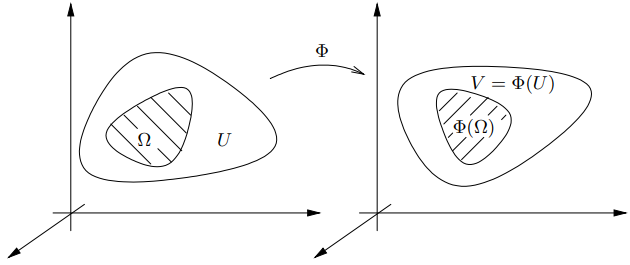
\includegraphics[width=1\linewidth]{Bilder/Substitutionsregel.png}
            \end{center}
        \end{minipage}
    \end{center}

    \subsubsection{Einschub: Verschiede Koordinatentransformationen}

    Die folgenden Koordinatentransformationen sind ein Diffeomorphismus, wie von der Substitutionsregel verlangt. \medskip


    \textbf{Polarkoordinaten}: $\Phi: (0, \infty) \times (-\pi,\pi) \to \R^2$ mit

    \begin{center}
        $\Phi(r, \varphi) := \begin{pmatrix}
                r \cos(\varphi) \\ r \sin(\varphi)
            \end{pmatrix}$ \quad und \quad $\det(d\Phi_{(r, \varphi)}) = r$
    \end{center}

    Desweiteren gilt: Bild($\Phi) = \R^2 \setminus \{(x,y) \in \R^2; \, y = 0, x \leq 0\}$. \medskip

    \textbf{Zylinderkoordinaten}: $\Phi: (0, \infty) \times (-\pi,\pi) \times \R \to \R^3$ mit

    \begin{center}
        $\Phi(r, \varphi, h) := \begin{pmatrix}
                r \cos(\varphi) \\ r \sin(\varphi) \\ h \\
            \end{pmatrix}$ \quad und \quad $\det(d\Phi_{(r, \varphi,h)}) = r$
    \end{center}

    Desweiteren gilt: Bild($\Phi) = \R^3 \setminus \{(x,y,z) \in \R^3; \, y = 0, x \leq 0\}$. \medskip

    \textbf{Kugelkoordinaten}: $\Phi: (0, \infty) \times (0,\pi) \times (-\pi,\pi) \to \R^3$ mit

    \begin{center}
        $\Phi(r, \Theta, \varphi) := \begin{pmatrix}
                r \sin(\Theta) \cos(\varphi) \\ r \sin(\Theta) \sin(\varphi) \\ r \cos(\Theta) \\
            \end{pmatrix}$ \quad und \quad $\det(d\Phi_{(r, \Theta, \varphi)}) = r^2 \sin(\Theta)$
    \end{center}

    \begin{center}
        \begin{minipage}{0.5\linewidth}
            \begin{center}
                Desweiteren gilt: Bild($\Phi) = \R^3 \setminus \{(x,y,z) \in \R^3; \, y = 0, x \leq 0\}$.
            \end{center}
        \end{minipage}
        \begin{minipage}{0.49\linewidth}
            \begin{center}
                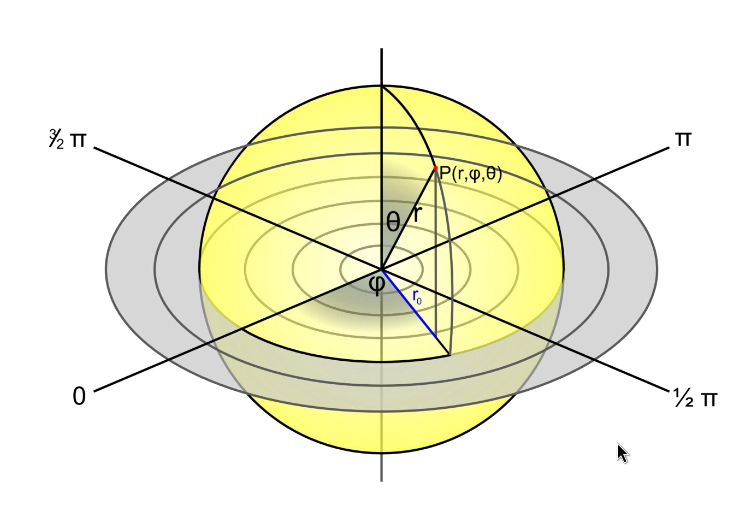
\includegraphics[width=1\linewidth]{Bilder/Kugelkoordinaten.png}
            \end{center}
        \end{minipage}
    \end{center}
    \subsection{Oberflächenmass und Flussintegral}
    %https://video.ethz.ch/lectures/d-math/2022/spring/401-0232-00L/25701150-98ca-4c82-a6fe-f812ac4074a9.html

    \subsubsection{Der Oberflächeninhalt}

    Sei $\Phi: U \subset \R^2 \to \R^3$ eine lokale Immersion. Sei $\overline{\Omega} \subset U$ beschränkt und Jordan messbar.\\

    Die Parametrisierung der Oberflaeche wird als Einbettung gegeben: Sei $\psi \in C^1(Q, \R)$ wobei $Q = [a,b] \times [c,d]$ mit $\phi(x,y) := \begin{pmatrix}
            x \\ y \\ \psi(x,y) \\
        \end{pmatrix}$. $\phi(x,y)$ ist dann \emph{immer} eine lokale Immersion. \\
    Der 2-dimensionale Flächeninhalt von $S = \Phi(\overline{\Omega})$ ist
    \begin{center}
        \eqboxf{$\displaystyle \mu_2(\Phi(\Omega)) := \int_\Omega \underbrace{|| \partial_x \Phi \times \partial_y \Phi|| d\mu}_{=: d o} = \int_S do$}
    \end{center}

    wobei $do$ der \emph{skalare Flächeninhalt} bezüglich $\Phi$ ist.


    \subsubsection{Das Integral einer Funktion über eine Oberfläche}

    Sei $\Phi: U \subset \R^2 \to \R^3$ eine lokale Immersion. Sei $\overline{\Omega} \subset U$ beschränkt und Jordan messbar. Sei $S = \Phi(\Omega)$ das zugehörige Flächenstück in $\R^3$ und $f: \overline{S} \to \R$ stetig. Dann ist das Integral von $f$ auf $S$:

    \begin{center}
        \eqbox{$\displaystyle \int_S f do := \int_\Omega (f \circ \Phi) \cdot ||\partial_x \Phi \times \partial_y \Phi || d \mu$}
    \end{center}


    \subsubsection{Normalenvektor}

    Sei $\Phi: U \subset \R^2 \to \R^3$ eine lokale Immersion. Der Normaleinheitsvektor $n$ zur Fläche $\Phi(U) = S$ ist:

    \begin{center}
        \eqbox{$\vec{n} = \dfrac{\partial_x \Phi \times \partial_y \Phi}{|| \partial_x \Phi \times \partial_y \Phi ||}$}
    \end{center}
    \begin{example}
        \textbf{Anmerkung}
        \begin{enumerate}
            \item[1)] Der Normalenvektor ist ein Einheitsvektor.
            \item[2)] Der Normalenvektor steht senkrecht auf der Fläche.
            \item[3)] Der Normalenvektor ist das Vektorprodukt der Tangentialvektoren (Ableitung $\rightarrow$ Vektor Tangential zur Flaeche). Und steht daher senkrecht zur Fläche.
            \item[4)] Die allgemeine Funktionsdeterminante $\phi: \R^n \rightarrow \R^m$ ist $\sqrt[]{det((D\phi)^T \cdot D\phi)}$ im Fall von $\R^3 \rightarrow \R^2$ ist dies $\sqrt[]{det((D\phi)^T \cdot D\phi)} = || \partial_x \Phi \times \partial_y \Phi ||$
        \end{enumerate}
    \end{example}
    \subsubsection{Das Flussintegral}

    Sei $V = \begin{pmatrix}
            P \\ Q \\ R \\
        \end{pmatrix}$ ein stetiges Vektorfeld. Sei $\Phi: U \subset \R^2 \to \R^3$ eine lokale Immersion. Sei $\overline{\Omega} \subset U$ beschränkt und Jordan messbar. Dann ist der Fluss von $V$ durch die Fläche $S = \Phi(\overline{\Omega})$:

    \begin{center}
        \eqboxf{$\displaystyle \int_S V \cdot \vec{n} \, do = \int_\Omega (V \circ \Phi) \cdot \dfrac{\partial_x \Phi \times \partial_y \Phi}{|| \partial_x \Phi \times \partial_y \Phi ||} || \partial_x \Phi \times \partial_y \Phi || d \mu$}
    \end{center}




    \subsection{Der Satz von Stokes in $\R^3$}
    %https://video.ethz.ch/lectures/d-math/2022/spring/401-0232-00L/25701150-98ca-4c82-a6fe-f812ac4074a9.html @45min

    \subsubsection{Die Rotation eines $\R^3$ Vektorfeld}

    Sei ein Vektorfeld $V \in C^1(\R^3)$. Dann ist die \emph{Rotation} von $V$:

    \begin{center}
        $\text{rot}(V) = \nabla \times V = \begin{pmatrix}
                \partial_{x_1} \\ \partial_{x_2} \\ \partial_{x_3} \\
            \end{pmatrix} \times \begin{pmatrix}
                V_1 \\ V_2 \\ V_3 \\
            \end{pmatrix} = \begin{pmatrix}
                \partial_{x_2}V_3 - \partial_{x_3}V_2 \\ \partial_{x_3}V_1 - \partial_{x_1}V_3 \\ \partial_{x_1}V_2 - \partial_{x_2}V_1 \\
            \end{pmatrix}$
    \end{center}


    \subsubsection{Satz von Stokes}

    Sei $\Phi$ eine lokale Immersion von $U \subset \R^2 \to \R^3$. Sei $\overline{\Omega} \subset U$ in $C^1_{stw}$, Jordan messbar und beschränkt. Sei $V \in C^1(\R^3)$. Dann gilt:

    \begin{center}
        \renewcommand{\arraystretch}{1.25}
        \eqbox{\begin{tabular}{r l}
                $\displaystyle \int_{S = \Phi(\Omega)} \text{rot}(V) \cdot \vec{n} \,d o$ & $\displaystyle= \int_\Omega (\text{rot}(V) \circ \Phi) \cdot (\partial_x \Phi \times \partial_y \Phi) d\mu$                   \\
                                                                                          & $\displaystyle= \int_{\partial\Omega} (V \circ \Phi) \cdot \frac{d}{dt}(\Phi \circ \gamma) dt = \int_{\partial S} V d\vec{s}$ \\
            \end{tabular}}
    \end{center}

    In Worten: Der Fluss von $\text{rot}(V)$ durch eine Fläche gleicht der Zirkulation vom Vektorfeld $V$ seinem Rand entlang.

    \begin{center}
        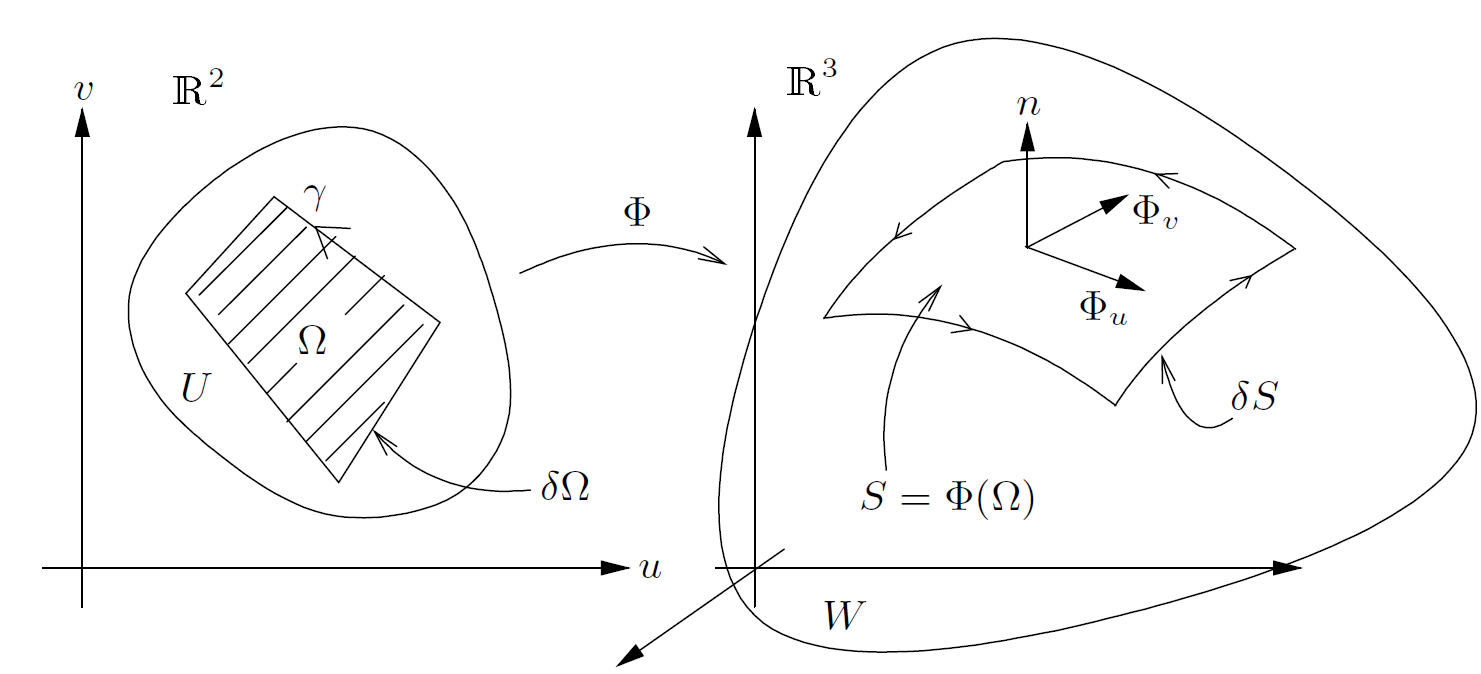
\includegraphics[width=0.75\linewidth]{Bilder/Stokes.png}
    \end{center}


    \subsection{Der Satz von Gauss}

    \subsubsection{Divergenz eines Vektorfeldes}

    Die Divergenz (''Quellstärke'') eines Vektorfeldes $V \in C^1(\R^3)$ ist:

    \begin{center}
        $\text{div}(V) = \partial_x V_1(x,y,z) + \partial_y V_2 (x,y,z) + \partial_z V_3 (x,y,z)$
    \end{center}

    \subsubsection{Satz von Gauss in $\R^2$}

    Sei $\Omega$ ein $C^1_{stw}$ Gebiet mit dem zu $\partial\Omega$ zugehörigen Tangentialvektor $\dot\gamma$. Sei $\nu$ der Normalvektor zum Rand (''äussere Normale''). Dann gilt:

    \begin{center}
        \begin{minipage}{0.4\linewidth}
            \begin{center}
                $\nu  = \begin{pmatrix} \dot \gamma_2 \\ - \dot\gamma_1 \\
                    \end{pmatrix} \dfrac{1}{\sqrt{\dot\gamma_1^2 + \dot\gamma_2^2}}$
            \end{center}
        \end{minipage}
        \begin{minipage}{0.59\linewidth}
            \begin{center}
                \eqbox{$\displaystyle \int_\Omega \text{div}(V) = \int_{\partial\Omega} V \cdot \nu \, d\vec{s}$}
            \end{center}
        \end{minipage}
    \end{center}

    \subsubsection{Satz von Gauss in $\R^3$}

    Sei ein Vektorfeld $V \in C^1(\R^3)$. Sei $\psi \in C^1(Q := [a,b] \times [c,d], \R_+)$ mit dem Hypographen $\Omega_{\psi} = \{x \in \R^3; (x_1,x_2) \in Q, 0  \leq x_3 \leq \psi(x_1,x_2)\}$. Wir setzen vorraus, dass $V = 0$ für $x_3 \leq 0$ und für $(x_1,x_2) \not\in Q$. Es gilt:

    \begin{center}
        \eqbox{$\displaystyle \int_{\Omega_\psi} \text{div}(V) d\mu = \int_Q V(\Phi) \cdot (\partial_x \Phi \times \partial_y \Phi)\, d\mu$} $\phi(x,y) := \begin{pmatrix}
                x \\ y \\ \psi(x,y) \\
            \end{pmatrix}$
    \end{center}

    In Worten: Das Integral von $\text{div}(V)$ in $\Omega_{\psi}$ gleicht dem Fluss von $V$ durch die Fläche von $\psi(x,y)$.






    \subsection{Beispiel intrinsischer Rand, Koorientierung, induzierte Orientierung des Randes und Flächeninhalt}

    Wir haben die Kugelkappe gegebn $\Sigma := \{x \in S^2 | x_3 \geq a\}$ mit $a \in (0,1)$
    Um die Fläche berechnen zu könnnen müssen wir die Kugelkappe parametrisieren. Dazu benutzen wir eine Einbettung:
    \begin{center}
        $\psi: \bar{B}^2_{\sqrt{1-a^2}} \rightarrow \R^3, \psi(y_1, y_2)=\begin{bmatrix*}
                y_1 \\ y_2 \\ \sqrt{1-y_1^2-y_2^2}
            \end{bmatrix*}$
    \end{center}
    1. Es muss nun gezeigt werden, dass $\psi$ eine Untermannigfaltigkeit ist. Daher muss gezeigt werden, dass $\psi$ eine Einbettung ist. Weil $\bar{B}^2_{\sqrt{1-a^2}}$ eine Rand hat, ist es eine Untermannigfaltigkeit mit Rand (da eingeschränkt). \\
    2. Der intrinsische Rand ist der 1-dimensionale Rand der Kugelkappe. Dieser kann aus der globalen Parametrisierung bestimmt werden:
    \begin{center}
        $\partial\Sigma = \psi(\partial \bar{B}^2_{\sqrt{1-a^2}})=\{\begin{bmatrix}
                y_1 \\ y_2 \\ \sqrt{1-y_1^2-y_2^2}
            \end{bmatrix} | (y_1, y_2) \in \R^2, y_1^2+y_2^2=1-a$\}
    \end{center}
    Der Rand kann natürlich auch mit cos(t) sin(t) auf einer Höhe von a parametrisiert werden. \\
    3. Die Koorientierung ist gegeben durch ein Einheitsnormalvektor
    \begin{center}
        $v(\psi(z)) = \dfrac{\partial_{y1} \psi \times \partial_{y2} \psi}{|| \partial_{y1} \psi \times \partial_{y2} \psi ||}$
    \end{center}
    4. Die induzierte Orientierung des Randes ist gegeben durch die Koorientierung und die Parametrisierung des Randes.
    \begin{center}
        $T: \partial \bar{B}^2_{\sqrt{1-a^2}} \rightarrow \R^2, T(\psi(y)) = \frac{1}{||d\psi(y)\tilde{T}(y)||}d\psi(y)\tilde{T}(y)$ \\
        Wobei: $\tilde{T}(y) = \frac{1}{\sqrt{1-a^2}} \begin{bmatrix}
                -y_2 \\ y_1
            \end{bmatrix}$
    \end{center}
    $\tilde{T}$ ist die positive Orientierung auf dem Kreis $\bar{B}^2_{\sqrt{1-a^2}}$, sodass die Kreisscheibe immer zur Linken liegt.
    5. Der Flächeninhalt lässt sich mithilfe des Betrages des Einheitsnormalvektors berechnen \\

    \begin{small}
        \subsection{Punktmengen}

        Sei der Radius $r > 0$ und der Index 0 markiert das Zentrum. Dann gilt: \medskip

        Kreis: $K = \left\{(x, y)\in \mathbb{R}^2; (x-x_0)^2+(y-y_0)^2 = r^2 \right\}$ \medskip

        Kugel: $K = \left\{(x, y, z)\in \mathbb{R}^3; (x-x_0)^2+(y-y_0)^2+(z-z_0)^2 = r^2 \right\}$ \medskip

        Zylinder: $Z=\left\{(x, y, z)\in \mathbb{R}^3; (x-x_0)^2+(y-y_0)^2 =r^2, \, 0\le z \le h \right\}$ \medskip

        Kegel: $K=\left\{(x, y, z)\in \mathbb{R}^3; x^2+y^2 = \frac{r^2}{h^2}(h-z)^2 \right\}$ \medskip

        Ellipse: $E=\left\{(x, y)\in \mathbb{R}^2; \frac{(x-x_0)^2}{a^2}+\frac{(y-y_0)^2 }{b^2} = r^2 \right\}$ \medskip

        Ellipsoid: $E=\left\{(x, y, z)\in \mathbb{R}^3; \frac{(x-x_0)^2}{a^2}+\frac{(y-y_0)^2}{b^2} +\frac{(z-z_0)^2}{c^2} = r^2 \right\}$

        \subsection{Volumen eines Ellipsoid}

        Für eine Berechnung des Volumens eines Ellipsoids benutzt man die folgendermassen angepassten Kugelkoordinanten:

        \begin{center}
            $F(r, \Theta, \varphi) := \begin{pmatrix}
                    a \cdot r \sin(\Theta) \cos(\varphi) \\ b \cdot r \sin(\Theta) \sin(\varphi) \\ c \cdot r \cos(\Theta) \\
                \end{pmatrix}$ und $\det(dF_{(r, \Theta, \varphi)}) = abc \cdot r^2 \sin(\Theta)$
        \end{center}

        $\int_{E(a, b, c, R)} 1 d \mu=\int_{B_{R}(0)}|\det d F(x, y, z)| d z d y d x = abc \mu\left(B_{R}(0)\right)$

        \subsection{Kochrezepte}

        \subsubsection{Integralgrenzen von einem Hyper- und Hypograph bestimmen}

        \begin{enumerate}
            \item Die Variable für das äusserste Integral wählen (oft $x$), alle anderen Variablen in der Mengengleichung auf $0$ setzen. Nun kann man die Grenze für die erste Variable herauslesen.
            \item Die Variable vom zweitäussersten Integral (oft $y$) auswählen, alle anderen Variablen in der Menge \textbf{ausser die schon bestimmte Variable} auf $0$ setzen.
            \item[2.5] Analoger Schritt für die 3te Variable.
            \item Nun hat man die Integralgrenzen bestimmt und kann fortfahren mit der Berechnung vom Integral.
        \end{enumerate}


        \subsubsection{Kochrezept Volumenberechnung}

        \begin{enumerate}
            \item Das Integrationsgebiet $\Phi(\Omega)$ (bzw. Integrationsgrenzen) bestimmen in den passenden Koordinatentransformationen.

                  \textbf{Achtung}: Auf die Einschränkungen der Koordinatentransformation achten (z.B. $r \in ]0,\pi[$).
            \item[1.5] Evtl. bemerken, dass die Koordinatentransformation eine Halbebene nicht trifft, dies aber vernachlässigbar ist beim Transformationssatz.
            \item Den Transformationssatz anwenden ($\det(d\Phi)$ nicht vergessen).
        \end{enumerate}


        \subsubsection{Kochrezept Oberflächeninhalt}

        \begin{enumerate}
            \item Die Menge anschauen und bestimmen um was für ein Objekt es sich handelt, Skizzen helfen! \textbf{Man berechnet die Oberfläche stückweise}. Einfache Fläche, wie Kreisflächen, kann man direkt mit den bekannten Formeln berechnen.
            \item Schwerere Oberflächen muss man mit folgendem Vorgehen berechnen:
                  \begin{itemize}
                      \item Eine Achse vorläufig entfernen, d.h. Variable auf $0$ setzen in der Mengengleichung. Man schaut von nun an von dieser Achse aus auf das Objekt. (z.B.: Man entfernt $z$ $\Rightarrow$ man schaut von oben).
                      \item Skizze von dem neuen 2D-Gebiet erstellen und dann die Ungleichungen (am Ende die Integralgrenzen) der zwei übrig bleibenden Variablen für das 2D-Gebiet bestimmen.
                      \item Mit der ursprünglichen Mengengleichung eine Funktion $\psi(x,y)$ für die entfernte Variable bestimmen. \textbf{Achtung}: Es kann sein, dass hier zwei Funktionen herauskommen, in diesem Fall muss man den Oberflächeninhalt für \textbf{beide} berechnen (evtl. Symmetrie!).
                      \item Lokale Immersion der Form $\phi(x,y) := \begin{pmatrix}
                                    x \\ y \\ \psi(x,y) \\
                                \end{pmatrix}$ bilden.
                      \item Oberflächeninhalt(e) berechnen mit der bekannten Formel, das Integrationsgebiet ist das zuvor bestimmte 2D-Gebiet.
                  \end{itemize}
            \item \textbf{Alle} Oberflächeninhalt zusammenaddieren.
        \end{enumerate}

    \end{small}

    \subsection{Einfache Geometrieformeln}

    \begin{center}
        \renewcommand{\arraystretch}{1.5}
        \begin{tabular}{r l l} \toprule
                      & Fläche/Volumen              & Umfang/Oberfläche                      \\
            \midrule
            Kreis     & $A = \pi r^2$               & $U = 2 \pi r$                          \\
            Kugel     & $V = \frac{4}{3} \pi r^3$   & $S = 4 \pi r^2$                        \\
            Ellipsoid & $V = \frac{4}{3} \pi a b c$ &                                        \\
            Zylinder  & $V = \pi r^2 h $            & $S = 2\pi r h + 2\pi r^2$              \\
            Kegel     & $V = \frac{1}{3} \pi r^2 h$ & $S = \pi r^2 + \pi r \sqrt{h^2 + r^2}$ \\
            \bottomrule
        \end{tabular}
    \end{center}
    \section*{Anhang}

    \subsection{Integralsubstitutionen}
    \begin{small}
        \begin{align*}
             & \int \frac{g'(x)}{g(x)}\text{d}x                     & u(x) & =g(x)                         & \text{d}x & =\frac{\text{d}u}{g'(x)}          \\
             & \int f(g(x))\cdot g'(x)\text{d}x                     & u(x) & =g(x)                         & \text{d}x & =\frac{\text{d}u}{g'(x)}          \\
             & \int f(e^x, \sinh(x), \cosh(x))\text{d}x             & u(x) & =e^x                          & \text{d}x & =\frac{\text{d}u}{e^x}            \\
             & \int f(x, \sqrt{1-x^2})\text{d}x                     & x    & =\sin(u)                      & \text{d}x & =\cos(u)\text{d}u                 \\
             & \int f(x, \sqrt{1+x^2})\text{d}x                     & x    & =\sinh(u)                     & \text{d}x & =\cosh(u)\text{d}u                \\
             & \int f(x, \sqrt{x^2-1})\text{d}x                     & x    & =\cosh(u)                     & \text{d}x & =\sinh(u)\text{d}u                \\
             & \int f\left(\frac{1}{\sqrt{a^2-x^2}}\right)\text{d}x & u(x) & =\frac{x}{a}                  & \text{d}x & =a\text{d}u                       \\
             & \int f\left(\sqrt{1+\frac{1}{x^2}}\right)\text{d}x   & u(x) & =\sqrt{x^2-1}                 & \text{d}x & =\frac{\sqrt{x^2-1}}{x} \text{d}u \\
             & \int R(\sin(x), \cos(x))\text{d}x                    & u(x) & =\tan\left(\frac{x}{2}\right) & \text{d}x & =\frac{2}{1+u^2}\text{d}u
        \end{align*}
        \subsubsection*{Tangenssubstitution}

        Sei $t(x) = \tan(\frac{x}{2})$ mit $x \in ]-\pi, \pi[$. Dann gilt

        \begin{center}
            \renewcommand{\arraystretch}{1.5}
            \begin{tabular}{l l} \toprule
                $\cos(x) = \dfrac{1 - t^2(x)}{1 + t^2(x)}$ & $\sin(x) = \dfrac{2 t(x)}{1 + t^2(x)}$   \\
                $\cos^2(x) = \dfrac{1}{1 + t^2(x)}$        & $\sin^2(x) = \dfrac{t^2(x)}{1 + t^2(x)}$ \\
                \bottomrule
            \end{tabular}
        \end{center}
    \end{small}
    \begin{center}
        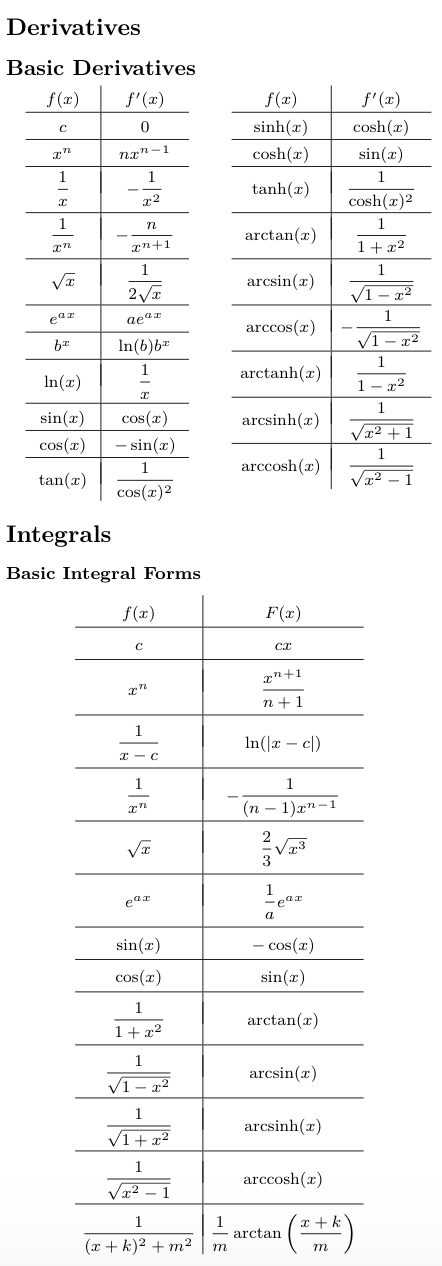
\includegraphics[width=0.9\linewidth, height=0.8\textheight]{Bilder/Integrals_1.png}
    \end{center}
    \begin{center}
        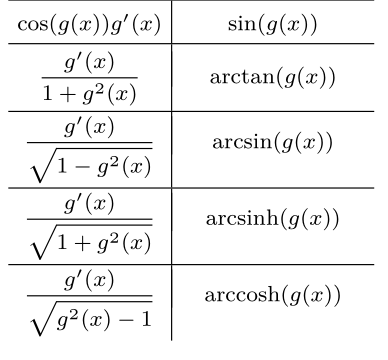
\includegraphics[width=0.6\linewidth, height=0.19\textheight]{Bilder/Integrals_2.png}
    \end{center}
\end{multicols*}
\begin{center}
    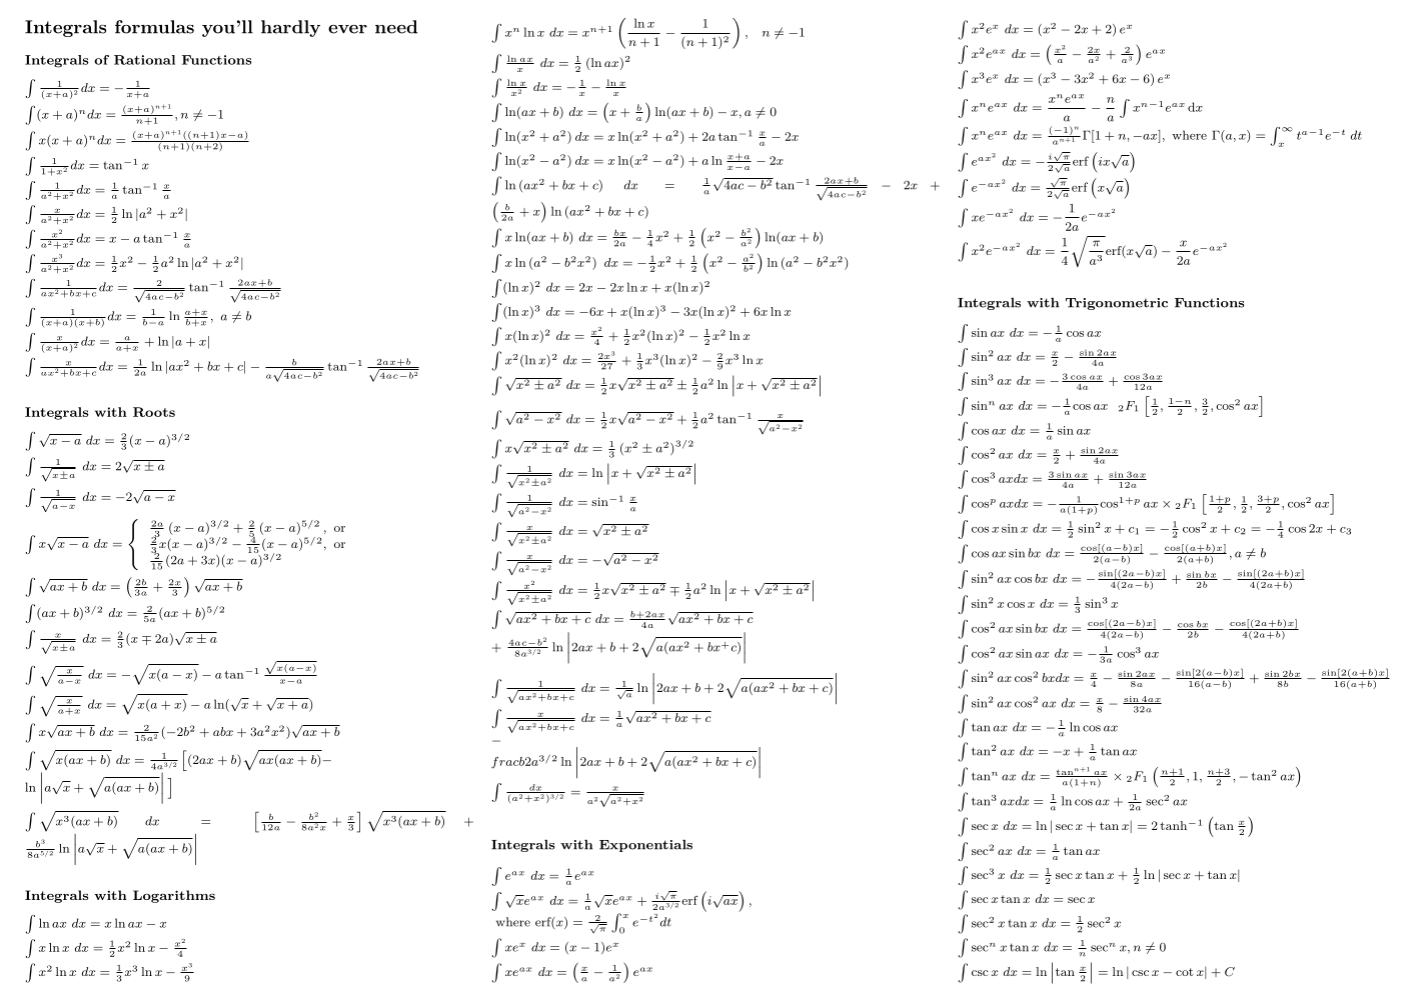
\includegraphics[height=0.98\textheight, width=\textwidth]{Bilder/Integrals_all.png}
\end{center}
\begin{center}
    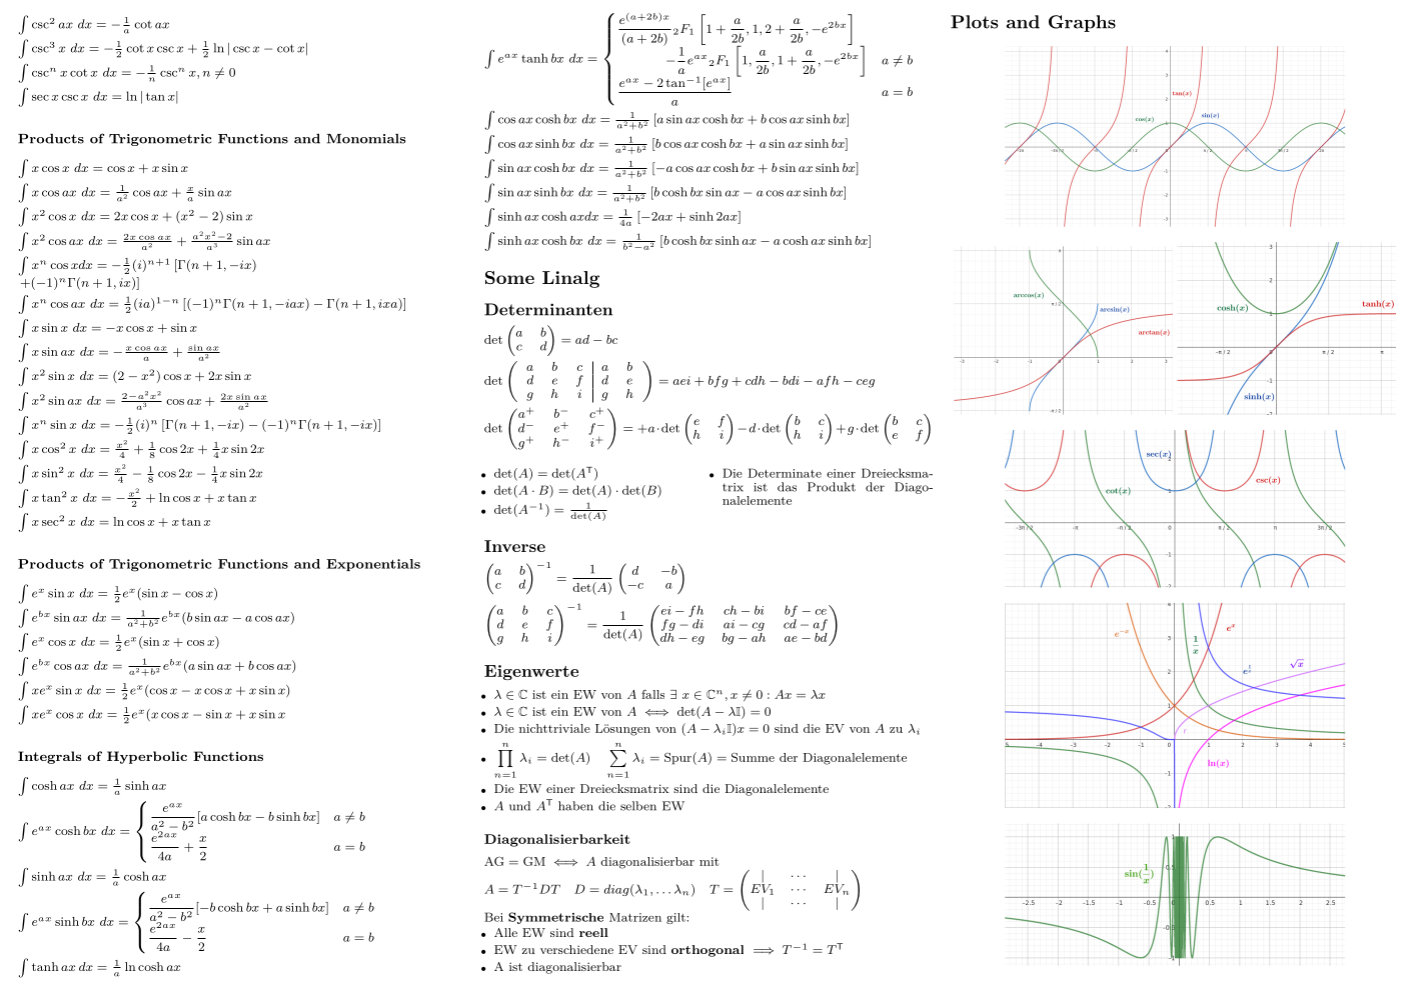
\includegraphics[height=0.98\textheight, width=\textwidth]{Bilder/Integrals_all_2.png}
\end{center}
\begin{center}
    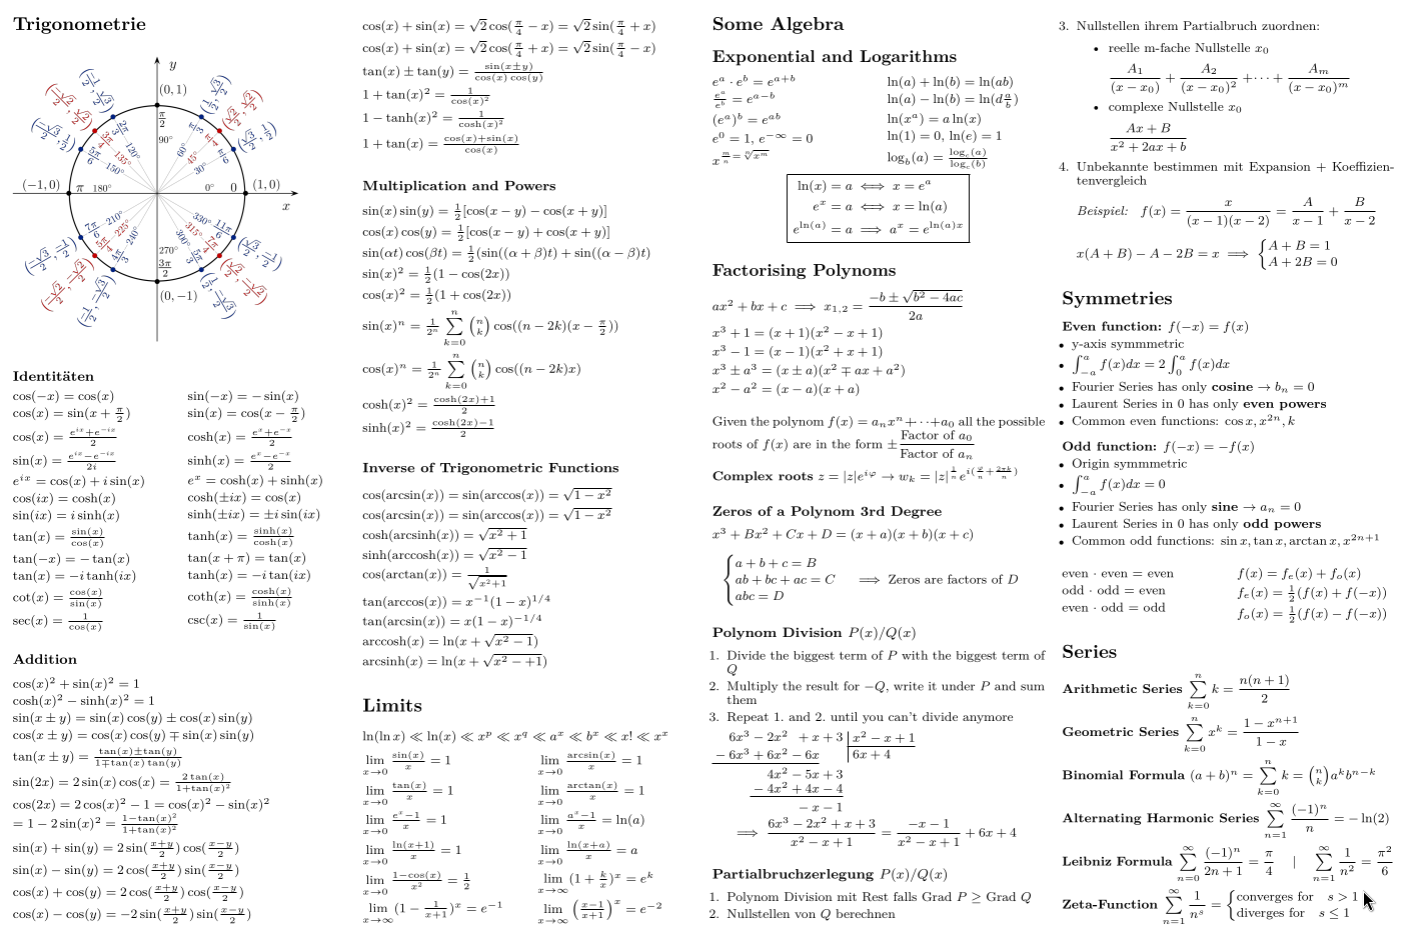
\includegraphics[height=0.98\textheight, width=\textwidth]{Bilder/Anhang_1.png}
\end{center}

\setcounter{secnumdepth}{2}
\end{document}